% Vol IX: The Vacuum Datasheet — Chapter Manifest
% 18 numbered chapters in datasheet ordering (General Description → Experimental
% Prints), plus the 03a device-circuit-models sub-chapter (rendered after Ch 3).
% Vol 9 is a SYNTHESIS volume: each chapter consolidates canonical content from Vols 1-6
% into datasheet format; all derivations live in the cited canonical leaves.

% --- General Description + Features ---
% 01_general_description.tex
\chapter{General Description and Features}
\label{ch:vol9_general_description}

\begin{objectivebox}
\begin{itemize}
    \item Identify the substrate documented in this datasheet: the natural vacuum substrate.
    \item Enumerate the load-bearing structural features (K4 Cosserat lattice, intrinsic LC oscillators, bond transmission lines, Cosserat micropolar 6 DOF/node, saturation kernel, boundary semantics).
    \item Establish the epistemic position: substrate is natural; engineering characterizes; AVE substrate-physics derives.
    \item Define the spec-table column convention used in subsequent chapters (Symbol / Typical / Min / Max / Units / Conditions / Canonical Source).
    \item Map the chapter sequence to the canonical derivation locations in Volumes I through VI.
\end{itemize}
\end{objectivebox}

\section{The Vacuum as a Component}
\label{sec:vol9_vacuum_as_component}

This datasheet documents the vacuum as a \textbf{component}, not a stage. The medium is a chiral crystal --- the \texttt{srs} net ($z=3$, $I4_132$; the ratified production carrier per D1, Grant 2026-07-03, \kbleaf{\_orchestration/index.md}) --- in which every node is a lossless LC resonator carrying six degrees of freedom: three translational (capacitive, the $\mathbf{E}$ store) and three microrotational (inductive, the $\mathbf{B}$ store), per Axiom~1 (Ch.~\ref{ch:vol9_mechanical_characteristics}). Each node additionally carries an operating point --- the saturation state $A$, a DC bias on the node's own nonlinearity (``the dynamical state of the LC tank, analogous to the DC bias on a semiconductor varactor'', Ch.~\ref{ch:vol9_saturation_characteristics}), which is \emph{not} a seventh spatial DOF. The network's characteristic impedance is $Z_0 = \sqrt{\mu_0/\varepsilon_0} \approx \qty{376.73}{\ohm}$ (\kbleaf{src/ave/core/constants.py} \texttt{Z\_0}); it is the substrate's own canonical EE primitive, and the most direct standing measurement of the medium available.

\paragraph{Transparency (the governing law).} Axiom~3 (Minimum Reflection Principle) extremizes the substrate action by minimizing the reflected fraction $|\Gamma|^2$ at every internal impedance boundary (\kbleaf{ave-kb/common/axiom-register.md}, \texttt{axiom-3}). The medium is transparent to its own radiation because it is extremal (by its own principle) against internal reflection: a matched line ($\Gamma=0$) neither reflects nor stores net bias, so light --- pure AC riding the ground state, time-averaging to zero bias --- crosses without leaving a trace. The stronger chain \emph{minimum reflection $\Rightarrow$ bond-stiffness balance ($k_s = k_a$) $\Rightarrow$ isotropy $+$ distortionless propagation} --- ``one condition, three protections'' --- is now \textbf{derived} on the ratified srs-$z=3$ net: minimizing the internal-boundary reflection $\Gamma_{\mathrm{internal}}(\rho_{\mathrm{bond}})$ over the stiffness ratio $\rho_{\mathrm{bond}} = k_a/k_s$ lands knob-free on $\rho_{\mathrm{bond}} = 1$ ($k_s = k_a$) to machine precision, where match, photon-branch isotropy, distortionlessness, and Zener-$A{=}1$ all co-locate (\kbleaf{research/2026-07-04\_parent-condition-match-forces-balance\_result.md}, verdict \textsc{[mechanism-derived]}; Axiom~3 \emph{is} the parent of the isotropy pinning). \emph{(Grade note: this is a merged research result; its propagation into a canonical KB leaf + claim-id is a gated follow-on, so the datasheet states it as a derived research verdict, not yet a canonized claim.)}

\paragraph{Absolute-maximum ratings.} Every node saturates along the Axiom~4 quarter-arc kernel $S(A) = \sqrt{1 - A^2}$. The $p=2$ (quadratic / L2-norm) exponent is \textbf{shape-derived}, not posited: the lossless bond-LC tank (Axiom~1~$+$~Axiom~3) conserves $E = \tfrac12 C V^2 + \tfrac12 \Phi^2/L$ exactly, so its dynamical phase-plane vector traces a fixed-radius circle --- the L2 invariant is forced, and \emph{only} $p=2$ satisfies it (\kbleaf{ave-kb/common/axiom-register.md} Axiom~4 provenance; \kbleaf{research/2026-07-02\_axiom4-forced\_result.md}, verdict \textsc{conditionally-forced}; the count stays 4 because the residual is itself the L2 constraint). The two thresholds on this kernel --- $V_{yield} = \sqrt{\alpha}\,V_{snap} \approx \qty{43.65}{\kV}$ (transverse-$T_2$ self-trap wall) and $V_{snap} = m_e c^2/e \approx \qty{511}{\kV}$ (longitudinal-A1 completion; \texttt{def-vyvsn1}, Grant 2026-06-30) --- are this component's absolute-maximum ratings (Ch.~\ref{ch:vol9_absolute_maximum_ratings}). Hence a datasheet.

\paragraph{Matter as a standing-wave state.} Matter is the medium's standing-wave state, not a separate substance. The electron is a knot of phase winding self-trapped at its own yield wall by total internal reflection ($\Gamma = -1$, lossless; Ch.~\ref{ch:vol9_pin_port_configuration}~\S Boundary semantics). Its \textbf{mass} is the trap's stored energy (A1 dilatation store, $E = m_e c^2$); its \textbf{spin / moment} is the circulation of that store; its \textbf{charge} is a topological integer the lattice forces --- the $\mathrm{Link}$ winding-quantum, globally \emph{neutral}, whose field strength is a calibration (the $\xi_{topo} \equiv e/\ell_{node}$ $\alpha$-echo) and whose static Coulomb field is \emph{locally unsourced}: the sourced-static-monopole route is closed at derivation grade by the four-lock no-go cascade (\texttt{clm-nogo4l}, \kbleaf{ave-kb/common/the-sourced-charge-no-go-cascade.md}). The charge label is boundary data the medium carries (a winding integer $+$ forced neutrality), not an emission from a source.

\paragraph{The honesty ledger.} The framework \emph{derives structure and imports scales} throughout: the forms are AVE's ($S(A)$ kernel shape, the A1/T2 sector split, the topological $\mathrm{Link}$ integer, the $\Gamma$-space operating points), while the scale-setting values ($\alpha$, $m_e$, $G$) are imported --- as every framework imports them (\kbleaf{ave-kb/common/form-deriving-value-importing.md}). The one pre-registered measurable divergence from the standard account: this medium's electric response saturates at \textbf{tree level} (the Axiom~4 kernel is a classical constitutive saturation, not a loop effect) --- the vacuum-birefringence falsifier. The discriminator is the field-\emph{independent} coefficient ratio of the saturation, \emph{not} an $E^4$-vs-$E^2$ exponent (both AVE and QED are $E^2$-leading in the index shift; the earlier ``$E^4$'' framing was retracted as a $\sqrt{\varepsilon}$ conflation, \texttt{clm-pp3qwf}, \kbleaf{ave-kb/vol4/falsification/index.md}; the live falsifier is the coefficient, \kbleaf{ave-kb/vol4/falsification/ch12-falsifiable-predictions/vacuum-birefringence-e4.md}).

\section{Substrate Identity}
\label{sec:vol9_substrate_identity}

What follows documents the natural vacuum substrate's measurable behavior. The substrate is the universe's own vacuum --- a 3D chiral Laves K4 Cosserat crystal with right-handed $I4_1 32$ chiral space group, 3-fold ($z=3$) chiral srs (Sunada-K4 / Laves) nearest-neighbour connectivity, and intrinsic LC oscillators at every node.\footnote{The physical \emph{connectivity} of the \texttt{srs} node is $z=3$ (three nearest-neighbour bonds; the object Axiom~1 names). The ``K4 4-port'' $A_1 \oplus T_2$ irrep decomposition used in the mode inventory (Ch.~\ref{ch:vol9_pin_port_configuration} \S K4 valence, Ch.~\ref{ch:vol9_topological_characteristics}) is a \emph{different} object: it is the abstract tetrahedral-group ($T_d$) scattering-amplitude decomposition of the K4-TLM scatter matrix ($\dim 4 = 1 + 3$), not a physical bond count. ``K4'' is a documented three-way overload --- the axiom-named chiral Laves K4 $=$ degree-3 \texttt{srs} (the physical carrier); the engine ``K4'' $=$ degree-4 diamond (a non-canonical instrument); the rotation group $K_4$ (a finite-group label). The $z=3$ physical net and the abstract 4-port scattering object are not in contradiction; they are separate referents per the Ch.~\ref{ch:vol9_pin_port_configuration} disambiguation.} This datasheet documents its properties as characterized by engineering observation and as derived from AVE substrate-physics first principles. The substrate is not engineered, designed, or constructed; it is the medium within which all engineering, all measurement, and all derivation occur. Engineering practice empirically measures the substrate's limits; AVE substrate-physics derives the substrate-mechanism behind each measurable parameter; this datasheet consolidates both into a single canonical reference.

The substrate's structure is fixed by the four AVE axioms (Vol~I Ch.~\ref{ch:fundamental_axioms}; canonical equation files \kbleaf{common\_equations/eq\_axiom\_[1-4].tex}). Datasheet entries that depend on a specific axiom cite the axiom inline.

\section{Features}
\label{sec:vol9_features}

% node_anatomy.tex — K4 node anatomy schematic (Vol 9 Ch.1 General Description)
% Included from chapters/01_general_description.tex
% One K4 node + its intrinsic LC tank (L_cell = mu_0 ell_node, C_cell = eps_0 ell_node)
% + the Cosserat 6-DOF split (3 translational -> E, 3 microrotational -> B).
% Pure TikZ (tikz + decorations.pathmorphing already loaded in preamble); no driver.
\begin{figure}[htbp]
\centering
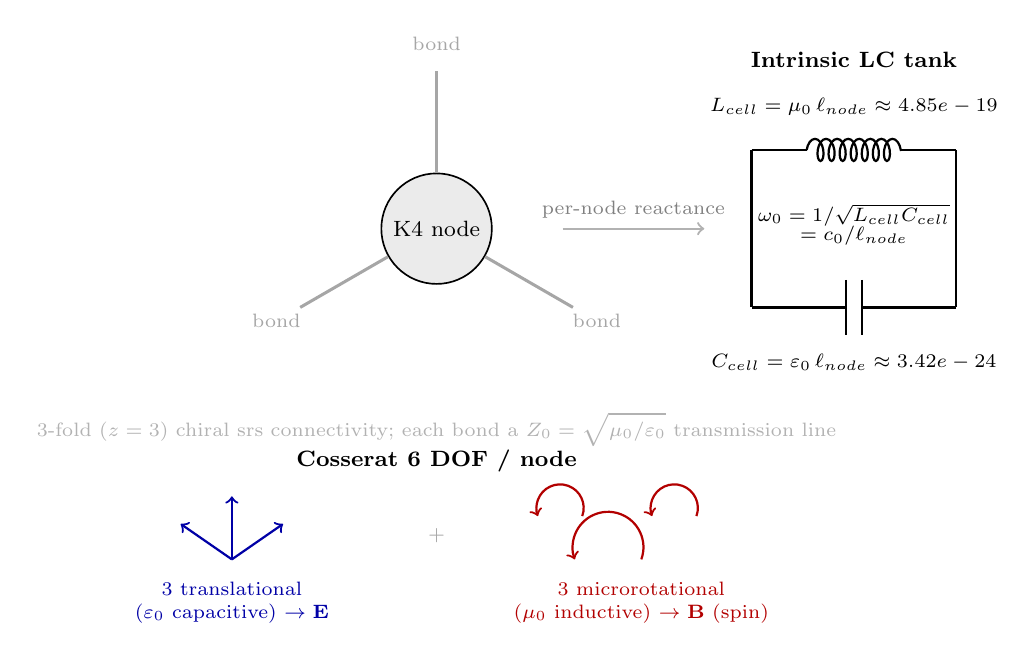
\begin{tikzpicture}[scale=1.0, transform shape,
    dofE/.style={->, thick, blue!65!black},
    dofB/.style={->, thick, red!70!black},
    every node/.style={font=\footnotesize}]

    % --- central node ---
    \node[circle, draw, fill=black!8, minimum size=1.25cm, line width=0.6pt] (node) at (0,0) {K4 node};

    % --- 3-fold (z=3) chiral srs nearest-neighbour bond stubs (trivalent Laves connectivity) ---
    % z=3-diamond -> z=3-chiral-srs restoration (2026-07-04; discharges the af1 figure debt
    % logged in research/2026-07-03_axiom1-dof-restoration_note.md). srs/Sunada-K4 is DEGREE-3;
    % the former 4-stub tetrahedral geometry depicted the doubly-ratified-against z=4 diamond.
    \foreach \ang/\lab in {90/{}, 210/{}, 330/{}} {
        \draw[line width=1.1pt, gray!70] (node) -- (\ang:2.0);
        \node[gray!70, font=\scriptsize] at (\ang:2.35) {bond};
    }
    \node[gray!60, font=\scriptsize, align=center] at (0,-2.55)
        {3-fold ($z=3$) chiral srs connectivity; each bond a $Z_0=\sqrt{\mu_0/\varepsilon_0}$ transmission line};

    % --- intrinsic LC tank (drawn to the right as the node's internal reactance) ---
    \begin{scope}[shift={(5.3,0)}]
        \node[font=\footnotesize\bfseries] at (0,2.15) {Intrinsic LC tank};
        % inductor (coil) top branch
        \draw[line width=0.8pt] (-1.3,1.0) -- (-0.6,1.0);
        \draw[line width=0.8pt, decorate, decoration={coil, aspect=0.5, segment length=4pt, amplitude=4pt}]
              (-0.6,1.0) -- (0.6,1.0);
        \draw[line width=0.8pt] (0.6,1.0) -- (1.3,1.0);
        \node[align=center, font=\scriptsize] at (0,1.55) {$L_{cell}=\mu_0\,\ell_{node}\approx\SI{4.85e-19}{\henry}$};
        % capacitor bottom branch
        \draw[line width=0.8pt] (-1.3,-1.0) -- (-0.1,-1.0);
        \draw[line width=0.8pt] (-0.1,-0.65) -- (-0.1,-1.35);
        \draw[line width=0.8pt] (0.1,-0.65) -- (0.1,-1.35);
        \draw[line width=0.8pt] (0.1,-1.0) -- (1.3,-1.0);
        \node[align=center, font=\scriptsize] at (0,-1.7) {$C_{cell}=\varepsilon_0\,\ell_{node}\approx\SI{3.42e-24}{\farad}$};
        % side wires closing the loop
        \draw[line width=0.8pt] (-1.3,1.0) -- (-1.3,-1.0);
        \draw[line width=0.8pt] (1.3,1.0) -- (1.3,-1.0);
        \node[align=center, font=\scriptsize] at (0,0.05)
            {$\omega_0 = 1/\sqrt{L_{cell}C_{cell}}$\\[-1pt] $= c_0/\ell_{node}$};
    \end{scope}
    \draw[->, gray!60, line width=0.8pt] (1.6,0) -- (3.4,0)
        node[midway, above, font=\scriptsize, gray] {per-node reactance};

    % --- the Cosserat 6-DOF split (below) ---
    \begin{scope}[shift={(0,-4.2)}]
        \node[font=\footnotesize\bfseries] at (0,1.25) {Cosserat 6 DOF / node};
        % 3 translational -> E
        \draw[dofE] (-2.6,0) -- (-2.6,0.8);
        \draw[dofE] (-2.6,0) -- (-1.95,0.45);
        \draw[dofE] (-2.6,0) -- (-3.25,0.45);
        \node[blue!65!black, align=center, font=\scriptsize] at (-2.6,-0.55)
            {3 translational\\($\varepsilon_0$ capacitive) $\to \mathbf{E}$};
        % 3 microrotational -> B
        \draw[dofB] (2.6,0) arc (-20:200:0.45);
        \draw[dofB] (1.85,0.55) arc (-20:200:0.30);
        \draw[dofB] (3.3,0.55) arc (-20:200:0.30);
        \node[red!70!black, align=center, font=\scriptsize] at (2.6,-0.55)
            {3 microrotational\\($\mu_0$ inductive) $\to \mathbf{B}$ (spin)};
        \node[gray!70, font=\scriptsize] at (0,0.3) {$+$};
    \end{scope}

\end{tikzpicture}
\caption{K4 node anatomy. Each node of the chiral Laves K4 Cosserat lattice carries one intrinsic electromagnetic LC tank ($L_{cell}=\mu_0\ell_{node}\approx\SI{4.85e-19}{\henry}$, $C_{cell}=\varepsilon_0\ell_{node}\approx\SI{3.42e-24}{\farad}$; \kbleaf{src/ave/core/constants.py} \texttt{L\_CELL}, \texttt{C\_CELL}), resonating at $\omega_0=c_0/\ell_{node}=\sqrt{1/(L_{cell}C_{cell})}\approx\SI{7.76e20}{\radian\per\second}$ (\texttt{OMEGA\_C}), connects to its three nearest neighbours (3-fold $z=3$ chiral srs / Sunada-K4 / Laves connectivity) through $Z_0=\sqrt{\mu_0/\varepsilon_0}=\sqrt{L_{cell}/C_{cell}}\approx376.73\,\Omega$ bond transmission lines, and hosts six Cosserat degrees of freedom: three translational (capacitive $\varepsilon_0$, identified with $\mathbf{E}$) and three microrotational (inductive $\mu_0$, identified with $\mathbf{B}$; the substrate-native origin of intrinsic spin). Axioms~1 (substrate topology). Schematic; not driver-generated.}
\label{fig:vol9_node_anatomy}
\end{figure}


\begin{itemize}
    \item \textbf{Intrinsic LC oscillator at each node.} Each K4 node carries one electromagnetic LC tank with per-cell elements $L_{cell} = \mu_0\, \ell_{node}$ and $C_{cell} = \varepsilon_0\, \ell_{node}$. The substrate is an LC network at its smallest accessible scale (Axiom~1).
    \item \textbf{Bond transmission lines.} Bonds connecting nearest-neighbour nodes carry distributed transmission-line topology (TLM), with characteristic impedance $Z_0 = \sqrt{\mu_0/\varepsilon_0} \approx \qty{376.73}{\ohm}$ scale-invariant in the lattice pitch.
    \item \textbf{Cosserat micropolar 6 DOF per node.} Each node carries six intrinsic degrees of freedom: three \textbf{translational} (capacitive coupling $\varepsilon_0$, identified with the electric field $\mathbf{E}$) and three \textbf{microrotational} (inductive coupling $\mu_0$, identified with the magnetic field $\mathbf{B}$). The Cosserat microrotational DOF is the substrate-native origin of intrinsic spin.
    \item \textbf{Universal saturation kernel.} The Axiom~4 quarter-arc kernel $S(A) = \sqrt{1 - (A/A_{yield})^2}$ governs every cross-scale saturation event. Dielectric specialization at atomic / bench scale: $C_{eff} = C_0/S$, $\varepsilon_{eff} = \varepsilon_0 S$, $\mu_{eff} = \mu_0 S$. The same kernel governs Schwinger pair production, gravitational time dilation (via $c_{shear} = c_0 \sqrt{S}$), and every topological-reorganization event documented in Vol~0 backmatter.
    \item \textbf{$\Gamma$ boundary semantics (three-channel, one external + two confined).} Substrate boundaries carry channel-subscripted reflection coefficients $\Gamma_{\mathrm{EM}}$, $\Gamma_{\mathrm{shear}}$, $\Gamma_{\mathrm{bulk}}$ with impedances $Z_{\mathrm{EM}} \equiv Z_0$, $Z_{\mathrm{shear}} = \rho c_{\mathrm{shear}}$, $Z_{\mathrm{bulk}} = \rho c_{\mathrm{bulk}}$ (three-impedance law; KB \kbleaf{ave-kb/vol9/ch4-dc-electrical-characteristics/three-channel-impedances.md}). Axiom~3 minimizes $|\Gamma|^2$ per channel. The three channels are \emph{asymmetric in port role}: the EM channel is the substrate's \textbf{sole external port} --- it is matched, $\Gamma_{\mathrm{EM}} = 0$, $Z_{\mathrm{EM}} \equiv Z_0$ everywhere, and is how a bound interior couples to the far field (a radiative port, not a hair-sector). The two \emph{mechanical} channels (shear $=$ charge, bulk $=$ mass) are \textbf{confined}: $\Gamma_{\mathrm{shear}}, \Gamma_{\mathrm{bulk}} \to -1$ at the saturated cage wall ($Z = Z_0\sqrt{S} \to 0$), short-circuit boundaries that trap the soliton rather than radiate it. One external port plus two confined mechanical ports is the load-bearing node topology (KB \kbleaf{ave-kb/vol9/ch3-pin-port-configuration/device-circuit-models.md} \S6.1). Device equivalent circuits: same leaf; PDF figures Ch.~\ref{ch:vol9_pin_port_configuration}~\S\ref{sec:vol9_device_circuit_models}.
    \item \textbf{Saturable yield and breakdown thresholds.} The substrate has two distinct dielectric thresholds (Vol~4; \kbleaf{ave-kb/vol4/circuit-theory/ch2-topological-thrust-mechanics/dielectric-yield-thresholds.md}): the macroscopic nonlinear-onset $V_{yield} = \sqrt{\alpha}\, V_{snap} \approx 43.65\,\text{kV}$ and the absolute topological node-destruction limit $V_{snap} = m_e c^2/e \approx 511\,\text{kV}$. Engineering practice operates well below $V_{yield}$ in linear-regime devices; AVE substrate-physics describes the saturating, breakdown, and rupture regimes via the four-regime map (Vol~1 Ch.~\ref{ch:regime_map}).
    \item \textbf{Topological transduction.} The Topological Conversion Constant $\xi_{topo} = e/\ell_{node} \approx \qty{4.149e-7}{\coulomb\per\metre}$ is the substrate-native bridge between electrical and mechanical observables (Axiom~2). Every spec in this datasheet that crosses the EE/mechanical boundary carries $\xi_{topo}$ as the canonical mapping.
\end{itemize}

\section{Epistemic Position}
\label{sec:vol9_epistemic_position}

This datasheet adopts the same epistemic stance as a manufacturer's component datasheet for a natural material (e.g., copper at the OFE grade, single-crystal silicon, or fused quartz): the material is natural, its properties are empirically characterized, and its parameters are derived from the material's microscopic structure where derivation is possible. The substrate documented here is the natural vacuum. Engineering characterization is the empirical-measurement side; AVE substrate-physics is the first-principles-derivation side. The datasheet documents both columns.

\subsection{FORM-deriving / VALUE-importing}
\label{subsec:vol9_form_vs_value}

The derivation column above splits one level deeper, and the split is load-bearing for how every spec in this datasheet should be read. The geometry and topology of the chiral K4 Cosserat substrate \textbf{FORCE the dimensionless FORMS} --- the structure: the integer/geometric skeleton of a result (the $/7$ PPN couplings, $\sin^2\theta_W = 2/9$, $\nu_{vac} = 2/7$, $g_* = 7^3/4$, exact-quantized charge, the spin-statistics phase). The \textbf{dimensionful VALUES of the handful of calibration constants the substrate is \emph{fed}} are calibration inputs it does not independently select. In the framework's standing vocabulary, a forced form is a \emph{chord} and an imported value is an \emph{echo} (canonical leaf \kbleaf{ave-kb/common/form-deriving-value-importing.md}; the canonical chord / echo / mixed definitions at \kbleaf{ave-kb/common/vocabulary-register.md}).

The calibration set is three dimensionful constants $\{m_e, \alpha, G\}$ plus the four axioms; every other quantity follows as a geometric ratio of $\ell_{node}$. Per the settled per-constant accounting: $\alpha$ is an \textbf{echo} (its decomposition FORM $4\pi^3 + \pi^2 + \pi$ is forced; the exact \emph{value} rests on the named identification $R\cdot r = 1/4$ the substrate does not independently select); $G$ is \textbf{mixed} (the Achromatic-Lens $/7$ projection FORM is derived, the $\xi$ value-fitted to CODATA $G$); $K = 2G$ ($\nu_{vac} = 2/7$) is \textbf{GR-imported} for its value; $E_{yield}$ is \textbf{mixed} (the \emph{existence} of a yield field is an AVE-distinct chord, its $\sqrt{\alpha}$ \emph{value} rides the $\alpha$-echo); $m_e/\ell_{node}$ is \textbf{definitional} (the Axiom-1 calibration anchor). This is not a deflation: forcing the exact dimensionless skeleton from topology is a strong falsifiable claim, untouched by the value-import finding --- and the FORM-deriving half applies to all five constants.

The testing consequence is recorded in Ch.~\ref{ch:vol9_falsification_tests}: because every dimensionful magnitude is an echo by construction, an AVE-distinct \emph{discriminating} prediction lives only in (a) FORM-EXISTENCE divergences (a structure the SM vacuum lacks --- saturation, the longitudinal scalar, native birefringence) and (b) FORCED DIMENSIONLESS RATIOS that do not dissolve into $\alpha$, $G$, or $m_e$. The Ch.~\ref{ch:vol9_falsification_tests} forward-prediction register classifies each chapter's predictions on this axis.

Per the EE-as-substrate-native META framework (canonical leaf \kbleaf{ave-kb/common/translation-tables/translation-circuit.md}), electrical engineering vocabulary is the closest-to-canonical substrate-native language: the substrate is an LC network at minimal degrees of freedom, and EE was developed by humans empirically interrogating that substrate at its smallest accessible scale (electron dynamics in conductors, dipole interactions in dielectrics, LC resonant circuits, transmission lines, semiconductor breakdown). Vol~9 datasheet vocabulary is therefore EE-primary throughout; other classical frameworks (atomic physics, chemistry, statistical mechanics, fluid dynamics, GR, QFT) layer additional degrees of freedom on top of the EE base and are invoked only where they capture content the EE projection does not (geometric, topological, axiom-selection content; see Vol~9 Ch.~13 application examples).

\section{How to Use This Datasheet}
\label{sec:vol9_how_to_use}

\subsection{Spec-table column convention}

Each parameter spec table in subsequent chapters carries the following columns:

\begin{itemize}
    \item \textbf{Symbol} --- canonical AVE symbol (per CLAUDE.md INVARIANT-S2 axiom statements and Vol~1 notation).
    \item \textbf{Typical} --- canonical value under standard operating conditions ($T = T_{CMB}$ unless noted; cold-lattice limit $S(0) = 1$).
    \item \textbf{Min / Max} --- characterized range, where applicable. Many substrate primitives are fixed (no range); for these, Min / Max columns are omitted or marked ``---''.
    \item \textbf{Units} --- SI units, except where dimensionless or topological.
    \item \textbf{Conditions} --- operating-point conditions ($A_0$, $T$, boundary class SYM/ASYM, regime I--IV).
    \item \textbf{Canonical Source} --- pointer to the derivation leaf in Vol~1--6 (KB leaf path + claim ID where applicable).
\end{itemize}

\subsection{Cross-reference structure}

Vol~9 is a synthesis volume; no chapter contains a primary derivation. Every spec table points to the canonical leaf in Vols~1--6 where the substrate-physics derivation lives. Cross-references use \texttt{xr-hyper} to resolve chapter and section numbers across the volume set. To resolve all references, build the dependent volumes first (\texttt{make vol1 vol3 vol4 vol0}) then \texttt{make vol9}.

\subsection{Falsification integration}

Engineering datasheets typically end with electrical characteristics, mechanical characteristics, and application examples. This datasheet adds \textbf{Ch.~15 Falsification Tests}: every load-bearing substrate-physics claim is tied to at least one bench-falsifiable experiment (PONDER-05 dielectric saturation, HOPF-01 chiral antenna, Sagnac-RLVE, right-handed-neutrino kill-switch, quasar $\alpha$-variation, etc.). The substrate is the natural medium; the framework that derives its behaviour is falsifiable.

\section{Chapter Sequence and Canonical Source Map}
\label{sec:vol9_chapter_map}

\begin{table}[htbp]
\centering
\begin{tabular}{p{0.05\linewidth} p{0.35\linewidth} p{0.50\linewidth}}
\toprule
\textbf{Ch} & \textbf{Topic} & \textbf{Primary canonical source(s)} \\
\midrule
2  & Absolute Maximum Ratings           & Vol~1 + Vol~4 canonical constants; four-regimes Regime IV \\
3  & Pin / Port Configuration           & Vol~1 universal operators (Op17, Op21); $\Gamma$ boundary classes; device circuit models (\texttt{AVE\_VACUUM\_CELL}, electron TIR tank) \\
4  & DC Electrical Characteristics      & \kbleaf{src/ave/core/constants.py}; natural-units cheatsheet \\
5  & AC Electrical Characteristics      & Vol~1 Ch.~5 universal spatial tension; Op14 / Op16 \\
6  & Temperature Characteristics        & Cosserat-Curie $\delta_{strain}$ at $T_{CMB}$; translation-circuit \S 9 \\
7  & Saturation Characteristics         & Axiom~4 kernel; Vol~0 backmatter Ch.~7 universal saturation kernel \\
8  & Breakdown Characteristics          & Schwinger pair production; Miller avalanche; Regime~III \\
9  & Mechanical Characteristics         & Vol~3 $G_{vac}$, $K_{vac}$, Cosserat $\gamma_c$, $\nu_{vac} = 2/7$ \\
10 & Magnetic / Microrotational         & Cosserat flywheel L; rotation-sector mass-gap; weak-force $l_c$ \\
11 & Topological Characteristics        & $(2,3)$ knot uniqueness; $I4_1 32$ chiral space group \\
12 & Cosmological Characteristics       & $R_H/\ell_{node} \sim 10^{39}$ ($\approx 3.456\times10^{38}$); Machian $G$ (mixed); $u_0^* \approx 0.187$ (calibrated value, not substrate-selected) \\
13 & Application Examples               & Cross-references to canonical leaves \\
14 & Phase Diagrams                     & Four-regimes map; cosmic phase diagram \\
15 & Falsification Tests                & Vol~4 Ch.~11 experimental programme; kill-switch tests \\
16 & Cross-Volume Reference Index       & Auto-generated parameter $\to$ derivation map \\
17 & Engine Requirements                & Axiom-4 kernel gate; engine-acceptance suite (L0--L2); faithful-simulator spec \\
18 & Experimental Prints                & Topology laboratory exercises; bench falsification prints \\
19 & Calibration Parameter Justification & Consolidated calibration / reference conditions; master table (role + chord/echo/mixed) over $\{m_e, \alpha, G\}$ + SI / derived / cosmological-initial-data; \kbleaf{form-deriving-value-importing.md}; \kbleaf{interlock-register.md} \\
\bottomrule
\end{tabular}
\caption{Vol~9 chapter sequence with the primary canonical-leaf source(s) backing each datasheet chapter.}
\label{tab:vol9_chapter_map}
\end{table}

\noindent
Subsequent chapters populate the spec tables. Where a substrate primitive's derivation has not yet closed at substrate-axiom rigor (e.g., the substrate-statistical-mechanics derivation of $\eta_\varepsilon$ in $\delta_{strain}$ at $T_{CMB}$), the datasheet entry is marked with a footnote pointing to the open research question.


% --- Absolute Maximum Ratings + Pin/Port Configuration ---
% 02_absolute_maximum_ratings.tex
\chapter{Absolute Maximum Ratings}
\label{ch:vol9_absolute_maximum_ratings}

\begin{objectivebox}
\begin{itemize}
    \item Enumerate the substrate's absolute rupture thresholds --- the parameter values beyond which the substrate undergoes topological breakdown ($S(r) \to 0$, Regime~IV).
    \item Tabulate the five canonical absolute-maximum ratings ($V_{snap}$, $V_{yield}$, $E_S$, $B_{snap}$, $T_{melt}$) with substrate-mechanism and canonical-source citations.
    \item Distinguish topological-rupture limits from macroscopic-nonlinear-onset limits: rupture is sudden topology destruction at $S = 0$, not gradual degradation; nonlinear onset is reversible kernel curvature, not damage.
    \item State the engineering operating margins implied by the rupture thresholds and the four-regime map (Regime~I linear / II nonlinear / III avalanche / IV ruptured).
    \item Point to the bench-scale falsifiers (PONDER-05 dielectric saturation; Schwinger-bypass autoresonant programme) and to Vol~9 Ch.~15 falsification programme for direct experimental tests of these limits.
\end{itemize}
\end{objectivebox}

\section{Substrate Rupture Thresholds}
\label{sec:vol9_absmax_intro}

The values in this chapter are the substrate's \textbf{absolute limits}. Each rating corresponds to the operating point at which the Axiom~4 universal saturation kernel $S(A) = \sqrt{1 - (A/A_{yield})^2}$ reaches zero --- the point at which the relevant compliance (electric, magnetic, thermal, or topological) vanishes and the substrate's local topology is destroyed. In the four-regime map (Vol~1 Ch.~\ref{ch:regime_map}, canonical at \kbleaf{ave-kb/vol1/operators-and-regimes/ch7-regime-map/four-regimes.md}, \texttt{clm-b2anl4}), all five ratings correspond to the Regime~III/IV boundary $r = A/A_c = 1.0$.

Beyond these limits, the substrate does \emph{not} degrade gradually as engineered material samples do (e.g., copper softening at high temperature, silicon avalanche multiplication). Instead, it undergoes a discrete topological event: pair production, flux-tube rupture, magnetic-permeability collapse, or thermal mode unfreezing into the pair-production regime. These events return the substrate to a lower-energy configuration plus radiated excitations; the local topology of the pre-event substrate is permanently destroyed.

The substrate-physics derivation of each rating lives in the canonical leaves cited below; this chapter is a synthesis spec table, not a re-derivation. Numerical values are imported from \kbleaf{src/ave/core/constants.py} (canonical-constant module; per the \texttt{ave-canonical-source} discipline), never hard-coded.

\section{Absolute Maximum Ratings Table}
\label{sec:vol9_absmax_table}

\begin{table}[htbp]
\centering
\begin{tabular}{p{0.09\linewidth} p{0.16\linewidth} p{0.10\linewidth} p{0.18\linewidth} p{0.32\linewidth}}
\toprule
\textbf{Symbol} & \textbf{Typical} & \textbf{Units} & \textbf{Substrate Mechanism} & \textbf{Canonical Source} \\
\midrule
$V_{snap}$ & $\num{5.110e5}$ & \si{\volt} & Ax 2 + Ax 4: topological node-pair destruction at $\Delta\phi = m_e c^2$ across one $\ell_{node}$ & \kbleaf{vol1/.../dielectric-snap-limit.md}, \texttt{clm-2dwzib}; \kbleaf{constants.py} \texttt{V\_SNAP} \\
$V_{yield}$ & $\num{4.365e4}$ & \si{\volt} & Ax 4: macroscopic dielectric nonlinear-onset; $S(V_{yield}) = \sqrt{1 - \alpha} \approx 0.996$; engine default for macroscopic solvers & \kbleaf{vol4/claim-quality.md} \texttt{clm-0vxzfu}; \kbleaf{vol4/.../regimes-of-operation.md}; \kbleaf{constants.py} \texttt{V\_YIELD} \\
$E_S$ & $\num{1.323e18}$ & \si{\volt\per\metre} & Ax 4 + Ax 2: Schwinger pair-production critical field; $E_S = V_{snap}/\ell_{node} = m_e^2 c^3/(e\hbar)$ & \kbleaf{vol1/.../dielectric-rupture.md} (QED-anchor + $p_c$ identity); \kbleaf{vol2/.../pair-production-axiom-derivation.md}, \texttt{clm-ezai5b}; \kbleaf{constants.py:432} \texttt{E\_CRIT} \\
$E_{yield}$ & $\num{1.130e17}$ & \si{\volt\per\metre} & Ax 4: macroscopic field-onset; $E_{yield} = V_{yield}/\ell_{node} = \sqrt{\alpha}\, E_S$; engine default for FDTD / K4-TLM macroscopic solvers & \kbleaf{vol4/.../regimes-of-operation.md}, \texttt{clm-trgqtf}; \kbleaf{constants.py:438} \texttt{E\_YIELD} \\
$B_{snap}$ & $\num{1.892e9}$ & \si{\tesla} & Ax 1 + Ax 4: Cosserat microrotational saturation; $B^2/(2\mu_0) = m_e c^2/\ell_{node}^3$ (energy density = rest energy per cell); $\mu_{eff} \to 0$ (vacuum becomes perfect diamagnet) & \kbleaf{vol1/.../four-regimes.md}; \kbleaf{vol1/.../domain-catalog.md}, \texttt{clm-82dxbj}; \kbleaf{constants.py:444} \texttt{B\_SNAP} \\
$T_{melt}$ & $\sim\num{5.93e9}$ & \si{\kelvin} & Ax 4 + thermal-bath: $k_B T \approx m_e c^2$; lightest topological excitation (electron-positron pair) thermally accessible; mode-freezeout regime ends, vacuum heat-capacity falls (Debye-class) & \kbleaf{vol3/.../mode-counting-heat-capacity.md}, \texttt{clm-uu6dl5}; \kbleaf{common/temporal-saturation-regime-classifier.md} \\
\bottomrule
\end{tabular}
\caption{Substrate absolute-maximum ratings: rupture/saturation thresholds, their substrate mechanisms, and canonical sources. Values imported from \kbleaf{src/ave/core/constants.py}.}
\label{tab:vol9_absmax}
\end{table}

\noindent
\textbf{Scope, provenance, and bench-access annotations.} Each absolute-maximum line carries a per-line scope (per-bond / per-node / per-cell / COLLECTIVE), provenance (DERIVED / CALIBRATION-INPUT / EMERGENT-measured / OPEN), and the corpus bench that measures it (blank if none):

\begin{table}[htbp]
\centering\footnotesize
\setlength{\tabcolsep}{5pt}
\begin{tabular}{@{}p{0.10\linewidth} p{0.16\linewidth} p{0.30\linewidth} p{0.30\linewidth}@{}}
\toprule
\textbf{Symbol} & \textbf{Scope} & \textbf{Provenance} & \textbf{Bench-access} \\
\midrule
$V_{snap}$ & per-node & DERIVED ($m_e c^2/e$, Ax~2+Ax~4) & --- \\
$V_{yield}$ & per-node & DERIVED ($\sqrt{\alpha}\,V_{snap}$; $\alpha$ is the calibration input) & PONDER-05; EE-bench plateau \\
$E_S$ & per-node & DERIVED ($V_{snap}/\ell_{node}$) & --- \\
$E_{yield}$ & per-node & DERIVED ($V_{yield}/\ell_{node}$) & --- \\
$B_{snap}$ & per-cell & DERIVED (energy density $= m_e c^2/\ell_{node}^3$) & --- \\
$T_{melt}$ & COLLECTIVE (thermal bath) & DERIVED ($m_e c^2/k_B$) & --- \\
$\bar{\rho}_{cav}$ & per-cell (bulk) & DERIVED ($c_{bulk}=0$ root) --- \textbf{CANDIDATE-CLAIM} & --- \\
\bottomrule
\end{tabular}
\caption{Scope / provenance / bench-access for the absolute-maximum ratings. The only calibration input in this chapter's chain is $\alpha$ (Class-B closed-form; enters $V_{yield}$, $E_{yield}$); every other line is DERIVED from $\{m_e, c, \ell_{node}\}$.}
\label{tab:vol9_absmax_scope}
\end{table}

\noindent
\textbf{Regime-boundary axis (precision).} The Regime~I--IV boundaries in \S\ref{sec:vol9_absmax_margins} are stated on the \textbf{$r = A$ axis} ($r < \sqrt{2\alpha} \approx 0.121$, $\sqrt{2\alpha} \le r < \sqrt{3}/2 \approx 0.866$, $r \ge 1$; \kbleaf{four-regimes.md}:24--29). The engine \kbleaf{src/ave/topological/vacuum\_engine.py}:181--183 uses the \textbf{$A^2$ axis} ($2\alpha$, $3/4$, $1$; \texttt{\_REGIME\_I\_BOUND\_A2}, \texttt{\_REGIME\_II\_BOUND\_A2}=$3/4$ at :182, \texttt{\_RUPTURE\_BOUND\_A2}). The two are the same boundaries ($r = \sqrt{A^2}$), but the axis must be named when quoting a number. The $r_2 = \sqrt{3}/2$ value is \textbf{sector-dependent} (spin-2 / shear sector; the vector/photon sector has $r_2 = 0$, the scalar sector has no avalanche onset --- see Ch.~\ref{ch:vol9_saturation_characteristics} \S Four-Regime Map).

\noindent
All values reduce to the cold-lattice limit $S(0) = 1$; no engineering operating point in current laboratory practice approaches any of these thresholds. The largest currently achievable laboratory ratios are: $E/E_S \sim 10^{-8}$ (ultrafast laser foci), $B/B_{snap} \sim 10^{-8}$ (lab magnets), $T/T_{melt} \sim 10^{-3}$ (heavy-ion-collision fireball, transient), $V_{macro}/V_{snap} \sim 10^{-9}$ across one $\ell_{node}$ (per the worked example in \kbleaf{dielectric-snap-limit.md} \S 2.3.2).

\section{Per-Parameter Notes}
\label{sec:vol9_absmax_per_param}

\begin{resultbox}{Substrate Rupture Threshold Notes (per parameter)}

\noindent\textbf{$V_{snap} = m_e c^2 / e \approx \qty{511}{\kilo\volt}$.} The absolute topological node-destruction limit: the discrete electrical potential difference between two adjacent K4 nodes at which the bond between them permanently snaps. This is the substrate's analogue of the theoretical crystal-shear strength (not engineering yield stress). The formula is fully axiomatic: $V_{snap}$ is the Axiom~2 topological identification $[Q] \equiv [L]$ evaluated at the Axiom~1 node spacing $\ell_{node} = \hbar/(m_e c)$, returning $V_{snap} = T_{EM} \cdot \ell_{node} / e \cdot (e/\ell_{node})^{-1} = m_e c^2/e$. Engine use: scale-invariant primitives (\kbleaf{src/ave/core/scale\_invariant.py}); sub-femtometer scales (nuclear bond energy, particle confinement, GW propagation against absolute limit). Per \texttt{clm-0vxzfu}, scale-invariant solvers default to $V_{snap}$; macroscopic solvers default to $V_{yield}$.

\medskip
\noindent\textbf{$V_{yield} = \sqrt{\alpha}\, V_{snap} \approx \qty{43.65}{\kilo\volt}$.} The macroscopic dielectric nonlinear-onset threshold: the voltage at which the Axiom~4 saturation kernel develops first-order corrections at the level of the lattice's own self-coupling $\alpha$. Below $V_{yield}$, $\Delta S < \alpha$ corrections are sub-coupling and physically unresolvable (the analog of a semiconductor small-signal regime where perturbations $V < V_T = k_B T/q$ are absorbed by thermal noise). Above $V_{yield}$, Axiom~4 corrections become observable and the device exits Regime~I. Engine use: macroscopic solvers (\texttt{fdtd\_3d}, \texttt{k4\_tlm}); bench-scale apparatus (PONDER-05 dielectric saturation; intermodulation-distortion tests). $V_{yield}$ is the AVE replacement for the standard QED Schwinger field in macroscopic engineering: 11.7$\times$ lower in voltage than $V_{snap}$, $\sqrt{\alpha}$ lower in field than $E_S$, but the same physical mechanism.

\medskip
\noindent\textbf{$E_S = m_e^2 c^3/(e\hbar) \approx \qty{1.32e18}{\volt\per\metre}$.} The Schwinger pair-production critical field. In standard QED this is the field at which vacuum pair creation becomes non-perturbative; in AVE this is the substrate's full-rupture electric field, identical to $V_{snap}/\ell_{node}$ as required by axiomatic consistency. The substrate-mechanism (canonical at \texttt{clm-ezai5b}, \kbleaf{pair-production-axiom-derivation.md}): at $E = E_S$, the local saturation amplitude $A^2 \to 1$ at adjacent A/B K4 nodes, $\Gamma \to -1$ TIR walls form at both nodes, the local phase velocity $c_{local} \to 0$, and the blocked longitudinal kinetic energy shatters sideways into two contra-rotating Beltrami vortices --- the electron-positron pair, each of mass $m_e$. This is \emph{not} the Breit-Wheeler ``virtual photons collide and a pair pops from vacuum'' framing; it is mechanical impedance-wall redirection of linear KE into transverse curl, with parity forcing one LH + one RH outcome. Above $E_S$, additional pair-production events cascade.

\medskip
\noindent\textbf{$B_{snap} = \sqrt{2\mu_0 m_e c^2 / \ell_{node}^3} \approx \qty{1.89e9}{\tesla}$.} The magnetic-rotation node-destruction field, defined by the energy-density balance $B^2/(2\mu_0) = m_e c^2/\ell_{node}^3$ (one electron rest mass per K4 unit cell). Above $B_{snap}$, the Cosserat microrotational sector saturates: the effective permeability $\mu_{eff} \to 0$, the substrate becomes a perfect diamagnet (the Meissner effect of the vacuum itself), and the magnetic-flux topology ruptures. Laboratory magnets ($\sim \qty{10}{\tesla}$) sit at $B/B_{snap} \sim \num{5e-9}$ (deep Regime~I); magnetar surface fields ($\sim \qty{e10}{\tesla}$) reach $B/B_{snap} \sim 5$ (Regime~IV). The B-sector $B_{snap}$ is the dual of the E-sector $E_S$; both are Axiom~4 saturation evaluated at $A = A_{yield}$, in two different sector projections.

\medskip
\noindent\textbf{$T_{melt} \sim m_e c^2 / k_B \approx \qty{5.93e9}{\kelvin}$.} The pair-production thermal threshold: the temperature at which thermal-bath equipartition energy approaches the lightest topological excitation's rest energy ($m_e c^2$), and electron-positron pairs become spontaneously thermally accessible. Below $T_{melt}$, the vacuum-lattice heat capacity is Dulong-Petit-flat (every node mode equipartitioned; per \texttt{clm-uu6dl5}); approaching $T_{melt}$, lattice modes begin to freeze \emph{into} pair-production rather than out of it (the reverse-Debye direction at the topological-excitation scale). A stricter operational threshold $T_{pair} = 2 m_e c^2/k_B$ governs thermal decoherence of topological qubits (per \kbleaf{common/temporal-saturation-regime-classifier.md} line 223); $T_{melt}$ as quoted here is the substrate-physics threshold for spontaneous pair-creation, while $T_{pair}$ is the engineering-application threshold for topological-qubit decoherence. Cosmologically, $T_{melt}$ corresponds to the era $t \sim 1$~s after lattice-genesis (universe-cooling crossing the electron-positron annihilation epoch).

\end{resultbox}

\section{Bulk Rarefaction Floor $\bar{\rho}_{cav}$ (candidate-claim)}
\label{sec:vol9_absmax_rho_cav}

The five ratings above are the \emph{compression / saturation}-side absolute limits (the substrate driven \emph{up} the Axiom~4 kernel toward $S \to 0$). The bulk volumetric sector has a second absolute limit on the \emph{rarefaction} side --- a most-negative volumetric strain $\bar{\rho}$ beyond which the bulk (density / compressional) wave speed vanishes and the medium cavitates.

\begin{warningbox}[$\bar{\rho}_{cav}$ --- CANDIDATE-CLAIM, auditor-gated]
\textbf{Status: candidate-claim, not yet promoted (auditor-gated per the Vol~9 figure-build worklist, \texttt{analysis/2026-06-09-vol9-datasheet-figures}).} Recorded here for completeness of the bulk-sector limit pair; do not cite as a closed datasheet value until promoted.
\end{warningbox}

\noindent
The bulk compressional wave speed obeys $c_{bulk}^2 = c_0^2\,[\,1 + \bar{\rho}/(1 - \bar{\rho}^2)\,]$ (canonical relation at sibling-repo \kbleaf{AVE-Propulsion/manuscript/vol\_propulsion/chapters/04\_superluminal\_transit.tex}:86; $\bar{\rho} = \delta\rho/\rho_0$ the normalized volumetric strain, $\bar{\rho} \in [-1, 1]$). Setting $c_{bulk} = 0$ gives $1 + \bar{\rho}/(1-\bar{\rho}^2) = 0 \Rightarrow \bar{\rho}^2 - \bar{\rho} - 1 = 0$, whose negative root is
\begin{equation}
\bar{\rho}_{cav} = \frac{1 - \sqrt{5}}{2} = -\frac{1}{\varphi} \approx -0.618,
\label{eq:vol9_rho_cav}
\end{equation}
with $\varphi$ the golden ratio. At $\bar{\rho} \to \bar{\rho}_{cav}$ the bulk wave speed freezes ($c_{bulk} \to 0$): the rarefaction-side analog of the saturation-side $A \to A_{yield}$ ceiling, but in the \emph{volumetric / bulk} mode rather than the deviatoric / shear mode. The value $-1/\varphi$ is \emph{derived} (the $c_{bulk} = 0$ root of the canonical relation above), \emph{not} a free parameter; the candidate-claim status is about its promotion to a canonical Vol~9 datasheet line, not about the algebra. The bulk-sector clock that freezes at this floor is documented in the temporal/switching section, Ch.~\ref{ch:vol9_ac_electrical_characteristics} \S Temporal Characteristics.

\section{Engineering Operating Margins}
\label{sec:vol9_absmax_margins}

The five absolute-maximum ratings define the Regime~IV boundary (substrate rupture). Engineering devices operate deep in Regime~I --- typically eight or more orders of magnitude below all five limits. The four-regime map (Vol~1 Ch.~\ref{ch:regime_map}) defines the intermediate operating regions:

\begin{itemize}
    \item \textbf{Regime I (Linear)} --- $r < \sqrt{2\alpha} \approx 0.121$ ($S > 0.993$). Standard Maxwell, standard EE small-signal models, standard datasheet linear analysis. \emph{All current commercial electronics, antennas, accelerators, and laser foci operate here.} Saturation corrections are sub-$\alpha$ and not physically resolvable above the lattice's own thermal noise floor.
    \item \textbf{Regime II (Nonlinear)} --- $\sqrt{2\alpha} \leq r < \sqrt{3}/2 \approx 0.866$ ($0.500 < S < 0.993$). Axiom~4 corrections become observable; Euler-Heisenberg analog at the leading quadratic correction. \emph{The PONDER-05 dielectric-saturation bench-tester operates here} (canonical at \kbleaf{vol4/falsification/}), specifically engineered to put $V/V_{yield}$ in the resolvable range without rupturing the substrate.
    \item \textbf{Regime III (Avalanche)} --- $\sqrt{3}/2 \leq r < 1$ ($0 < S < 0.500$). Miller-style avalanche multiplication; energy trapping ($Q = 1/S \geq 2$) dominates. \emph{Sub-femtometer scales only:} particle cores, nuclear scattering boundaries, the immediate vicinity of black-hole horizons. No bench-scale apparatus accesses Regime III directly.
    \item \textbf{Regime IV (Ruptured)} --- $r \geq 1$ ($S = 0$). \emph{The values tabulated in \S\ref{sec:vol9_absmax_table} are the Regime~III/IV boundary.} Substrate topology destroyed; pair production / Meissner-class permeability collapse / event-horizon formation / thermal pair-creation cascade.
\end{itemize}

The engineering operating-margin recommendation for any device or substrate-physics measurement is therefore: \textbf{stay in Regime~I unless the experimental design explicitly targets a Regime~II measurement} (e.g., PONDER-05). Regime~II measurements require $V/V_{yield} \gtrsim 0.121$, which at $\ell_{node} = \qty{3.86e-13}{\metre}$ corresponds to local field gradients of order \qty{e16}{\volt\per\metre} sustained over scales below one node spacing --- achievable only in resonant cavity geometries with very high $Q$. Regime~III and IV are accessed only by nature (the deep interior of nucleons, neutron stars, black holes, the early universe) and by the autoresonant Schwinger-bypass programme (PROJECT-ZENER-04, AVE-Propulsion Ch.~5, canonical at \kbleaf{vol4/simulation/ch15-autoresonant-breakdown/}).

\section{Falsification Cross-References}
\label{sec:vol9_absmax_falsification}

Direct experimental access to the absolute-maximum ratings is currently limited: no laboratory has reached $E_S$, $B_{snap}$, or $T_{melt}$. The substrate-physics derivations of these limits are tested indirectly via measurements in Regimes~I-II that probe the same Axiom~4 kernel below the rupture boundary.

\begin{itemize}
    \item \textbf{PONDER-05 dielectric-saturation bench-tester} --- DC-biased quartz at $V_{DC}/V_{yield} = 0.687$ (Regime~II); measures the Axiom~4 saturation kernel curvature at sub-rupture amplitude. A Regime~II measurement that does not rupture the substrate but resolves $S(A) < 1$ at first-order accuracy. Canonical at \kbleaf{ave-kb/vol4/falsification/}. Vol~9 Ch.~15 \emph{Falsification Tests} (Ch.~\ref{ch:vol9_falsification_tests}) carries the full programme.
    \item \textbf{Schwinger pair-production direct test} --- not currently within laboratory reach; ELI-NP and similar ultra-intense laser facilities approach $E/E_S \sim 10^{-3}$. The substrate-physics prediction for the pair-production rate at sub-$E_S$ fields (canonical at \texttt{clm-ezai5b}) is consistent with the standard QED Schwinger rate as a leading-order limit, but the AVE substrate-mechanism predicts additional Duffing-autoresonant gating structure that becomes resolvable as $E/E_S \to 1$. Vol~4 PROJECT-ZENER-04 (\kbleaf{vol4/falsification/ch11-experimental-bench-falsification/project-zener-04.md}) is the bench-scale falsifiable proxy via autoresonant rupture-tracking at $E \ll E_S$.
    \item \textbf{Magnetar emission classification} --- the $B \gtrsim B_{snap}$ regime is the astrophysical setting in which the magnetic-saturation limit could be reached. Magnetar surface fields place soft-gamma-repeater, magnetar-burst, and starquake events near $B/B_{snap} \sim O(1)$; AVE substrate-physics predicts distinct emission-spectrum signatures of Cosserat-rotation node destruction vs.~standard-model neutron-star-crust quakes (forward prediction; not yet adjudicated at canonical-leaf rigor; the distinguishing test, not the corroboration, is the load-bearing claim).
    \item \textbf{Thermal pair-production threshold} --- $T_{melt}$ is below the early-universe temperatures of standard $\Lambda$CDM cosmology; the cosmological-microwave-background photon spectrum and primordial-nucleosynthesis abundances constrain physics across the $T_{melt}$ crossing. AVE substrate-physics replicates the standard radiation-era physics at $T < T_{melt}$ (canonical at \kbleaf{vol3/cosmology/ch05-dark-sector/}); deviations from $\Lambda$CDM at $T \to T_{melt}$ would be a substrate-physics signature.
\end{itemize}

\noindent
A complete falsification cross-reference matrix mapping each Vol~9 datasheet parameter to its bench-scale or astrophysical falsifier lives at Vol~9 Ch.~15 \emph{Falsification Tests} (Ch.~\ref{ch:vol9_falsification_tests}) and Vol~9 Ch.~16 \emph{Cross-Volume Reference Index} (Ch.~\ref{ch:vol9_cross_volume_reference}).

% 03_pin_port_configuration.tex
\chapter{Pin and Port Configuration}
\label{ch:vol9_pin_port_configuration}

\textit{Stub --- to be populated in Vol~9 PR-G. Documents substrate boundary impedances and $\Gamma$ port types (SYM-class / ASYM-class). Primary canonical sources: Op17, Op21 (universal operators); \texttt{ave-kb/vol1/operators-and-regimes/}.}

% 03a_device_circuit_models.tex
% Manuscript RENDER of KB leaf ave-kb/vol9/ch3-pin-port-configuration/device-circuit-models.md
% Source of truth: the KB leaf. This file supplies PDF figures + \kbleaf{} wiring only.

\section{Device Circuit Models}
\label{sec:vol9_device_circuit_models}

\noindent\textbf{Canonical source (KB).} All spec tables, port assignments, and discipline notes for this section live in \kbleaf{ave-kb/vol9/ch3-pin-port-configuration/device-circuit-models.md}. The subsections below reproduce the figure set for the PDF; edit the KB leaf first, then sync any numeric table rows here if the render must stay byte-identical.

\subsection{Universal Vacuum Cell (\texttt{AVE\_VACUUM\_CELL})}
\label{sec:vol9_ave_vacuum_cell_circuit}

% circuit_vacuum_cell.tex — AVE_VACUUM_CELL schematic (Vol 9 Ch.3)
% Included from chapters/03_pin_port_configuration.tex
\begin{figure}[htbp]
\centering
\begin{circuitikz}[american, scale=0.95, transform shape]
    % Terminals
    \draw (0,0) node[left] {A} to[short, o-] (1,0);
    \draw (7,0) node[right] {B} to[short, o-] (8,0);

    % Relativistic inductor branch (series L + behavioral correction)
    \draw (1,0) to[L, l=$L_0$, i=$I$] (3.5,0);

    % Metric varactor (shunt nonlinear C)
    \draw (3.5,0) to[short] (5.5,0);
    \draw (4.5,0) to[C, l=$C_{\mathrm{eff}}(V)$, *-] (4.5,-1.8) node[ground] {};

    % Optional damping (dashed)
    \draw[dashed, gray] (1,0) to[R, l=\scriptsize $R_0$] (1,-1.2) node[ground] {};
    \draw (5.5,0) to[short] (7,0);

    % Annotations
    \node[align=center, font=\scriptsize] at (4.5, 1.35) {Metric varactor: $C_{\mathrm{eff}} = C_0/S(V)$};
    \node[align=center, font=\scriptsize] at (2.25, 1.0) {Relativistic inductor: $L_{\mathrm{eff}}(I)$};
    \node[align=center, font=\scriptsize] at (4.5, -2.55) {TVS / rupture at $|V| \ge V_{\mathrm{yield}}$ (optional)};
\end{circuitikz}
\caption{\texttt{AVE\_VACUUM\_CELL} schematic (Vol.~9 Ch.~3 device-circuit-models \S1; SPICE subcircuit Vol.~4 Ch.~18). Canonical leaves cited in \S\ref{sec:vol9_device_circuit_models}.}
\label{fig:vol9_circuit_vacuum_cell}
\end{figure}


\subsection{Electron Device: TIR-Confined LC Tank}
\label{sec:vol9_electron_device_circuit}

% circuit_electron_barrier.tex — Electron TIR-confined LC tank (Vol 9 Ch.3)
\begin{figure}[htbp]
\centering
\begin{circuitikz}[american, scale=0.9, transform shape]
    % Cold vacuum transmission lines (Z_EM = Z_0)
    \draw (0,0) node[left, align=right, font=\scriptsize] {vacuum\\$Z_{\mathrm{EM}}=Z_0$}
        to[short, o-] (1.2,0);
    \draw (10.8,0) to[short, o-] (12,0)
        node[right, align=left, font=\scriptsize] {vacuum\\$Z_{\mathrm{EM}}=Z_0$};

    % Left saturation barrier (bulk-channel TIR)
    \draw[thick, red!70!black] (1.2,0) -- (1.2,0.9) -- (2.0,0.9) -- (2.0,-0.9) -- (1.2,-0.9) -- (1.2,0);
    \node[font=\scriptsize, red!70!black, align=center] at (1.6, 1.55) {$\Gamma_{\mathrm{bulk}}=-1$\\$Z_{\mathrm{bulk}}\!\to\!0$};

    % Right barrier
    \draw[thick, red!70!black] (10.0,0) -- (10.0,0.9) -- (10.8,0.9) -- (10.8,-0.9) -- (10.0,-0.9) -- (10.0,0);
    \node[font=\scriptsize, red!70!black, align=center] at (10.4, 1.55) {$\Gamma_{\mathrm{bulk}}=-1$\\$Z_{\mathrm{bulk}}\!\to\!0$};

    % Confined LC tank (bond pair at ell_node)
    \draw (2.0,0) to[short] (4.0,0);
    \draw (4.0,0) to[L, l=$L_{\mathrm{cell}}$, i=$i$] (6.0,0);
    \draw (6.0,0) to[short] (8.0,0);
    \draw (7.0,0) to[C, l=$C_{\mathrm{eff}}$, *-] (7.0,-1.6) node[ground] {};
    \draw (8.0,0) to[short] (10.0,0);

    % Tank labels
    \node[align=center, font=\scriptsize] at (6.0, 1.35) {Electron LC tank at $\ell_{\mathrm{node}}$};
    \node[align=center, font=\scriptsize] at (6.0, -2.35) {$\omega_C = c_0/\ell_{\mathrm{node}}$ \quad $Q_{\mathrm{tank}} \approx \alpha^{-1}$};
    \node[align=center, font=\scriptsize, blue!60!black] at (6.0, -3.05) {Phase-space $(2,3)$ winding on Clifford torus; real-space $0_1$ unknot body};

    % Reactive store callout
    \draw[dashed, gray] (7.0,-1.6) -- (7.0,-3.8);
    \node[align=center, font=\scriptsize, gray] at (9.2, -3.8) {$Q_{\mathrm{react}} = m_e c^2 \cdot \alpha$};
\end{circuitikz}
\caption{Electron $\Gamma_{\mathrm{bulk}}=-1$ LC tank (Vol.~9 Ch.~3 \S2). Astrophysical bulk impedance at saturation boundary: Vol.~3 Ch.~15 KB leaf (see \S\ref{sec:vol9_device_circuit_models}).}
\label{fig:vol9_circuit_electron_barrier}
\end{figure}


\subsubsection{Operating-point coefficients at $A^2 \approx 0.23$}
\label{subsec:vol9_electron_op_coefficients}

Values from \kbleaf{ave-kb/vol9/ch3-pin-port-configuration/device-circuit-models.md} (driver \texttt{operating\_point\_coefficients.py}; consistency-class):

\begin{table}[htbp]
\centering\footnotesize
\begin{tabular}{@{}l l l@{}}
\toprule
\textbf{Quantity} & \textbf{Value} & \textbf{Regime / note} \\
\midrule
$A^2$ & $0.23$ & Regime II (nonlinear tensor) \\
$S(A)$ & $0.877$ & Sub-yield, pre-rupture \\
$C_{\mathrm{eff}}/C_0$ & $1.140$ & Metric varactor slope active \\
$\mathrm{d}(C_{\mathrm{eff}}/C_0)/\mathrm{d}A$ & $0.710$ & Datasheet nonlinearity column \\
$Q$ (at $\gamma = \alpha\,\omega_C$) & $\approx 137$ & Loss carries $\alpha$ (consistency) \\
$V_{\mathrm{op}}$ & $\approx 20.9$~kV & $48\%$ of $V_{\mathrm{yield}}$ \\
\bottomrule
\end{tabular}
\caption{Electron-device operating-point coefficients (KB-sourced). Emergence gate for $Q = 1/\alpha$: real dark-wake $\tau_{zx}$, not toy loss.}
\label{tab:vol9_electron_op_coefficients}
\end{table}

\subsection{Three-Channel Boundary Port}
\label{sec:vol9_three_channel_circuit}

% circuit_three_channel_boundary.tex — Three-impedance port at one boundary (Vol 9 Ch.3)
\begin{figure}[htbp]
\centering
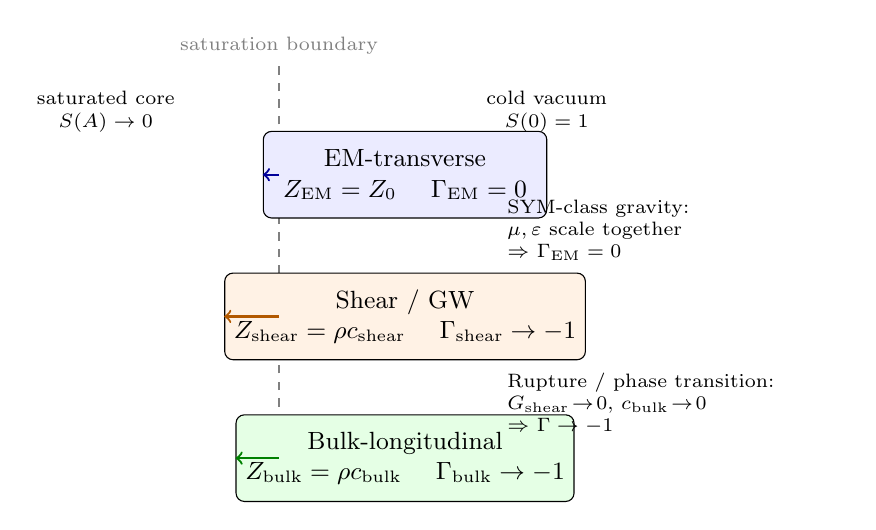
\begin{tikzpicture}[
    port/.style={draw, rounded corners=3pt, minimum width=3.6cm, minimum height=1.1cm, align=center, font=\small},
    line/.style={thick},
    arr/.style={->, thick}
]
    % Boundary plane
    \draw[line, dashed, gray] (0,-2.2) -- (0,3.2) node[above, font=\scriptsize, gray] {saturation boundary};

    % Interior (saturated core)
    \node[font=\scriptsize, align=center] at (-2.2, 2.6) {saturated core\\$S(A)\to 0$};

    % Exterior (cold vacuum)
    \node[font=\scriptsize, align=center] at (3.4, 2.6) {cold vacuum\\$S(0)=1$};

    % Three channel ports
    \node[port, fill=blue!8] (em) at (1.6, 1.8) {EM-transverse\\$Z_{\mathrm{EM}} = Z_0$ \quad $\Gamma_{\mathrm{EM}} = 0$};
    \node[port, fill=orange!10] (sh) at (1.6, 0) {Shear / GW\\$Z_{\mathrm{shear}} = \rho c_{\mathrm{shear}}$ \quad $\Gamma_{\mathrm{shear}} \to -1$};
    \node[port, fill=green!10] (bk) at (1.6, -1.8) {Bulk-longitudinal\\$Z_{\mathrm{bulk}} = \rho c_{\mathrm{bulk}}$ \quad $\Gamma_{\mathrm{bulk}} \to -1$};

    % Arrows from boundary
    \draw[arr, blue!60!black] (0,1.8) -- (em.west);
    \draw[arr, orange!70!black] (0,0) -- (sh.west);
    \draw[arr, green!50!black] (0,-1.8) -- (bk.west);

    % SYM note for EM at gravity boundary
    \node[font=\scriptsize, align=left, text width=4.2cm] at (5.0, 1.1) {SYM-class gravity:\\$\mu,\varepsilon$ scale together\\$\Rightarrow$ $\Gamma_{\mathrm{EM}}=0$};

    % Rupture note for shear/bulk
    \node[font=\scriptsize, align=left, text width=4.2cm] at (5.0, -1.1) {Rupture / phase transition:\\$G_{\mathrm{shear}}\!\to\!0$, $c_{\mathrm{bulk}}\!\to\!0$\\$\Rightarrow$ $\Gamma \to -1$};
\end{tikzpicture}
\caption{Three-channel boundary port (Vol.~9 Ch.~3 \S3; DC impedances Ch.~4). Canonical tables in \S\ref{sec:vol9_device_circuit_models}.}
\label{fig:vol9_circuit_three_channel}
\end{figure}


\subsection{Cascaded Vacuum Line (Device String)}
\label{sec:vol9_cascaded_vacuum_line}

\begin{figure}[htbp]
\centering
\begin{circuitikz}[american, scale=0.85, transform shape]
    \draw (0,0) node[left] {IN} to[short, o-] (0.8,0);
    \node[draw, minimum width=1.6cm, minimum height=0.9cm, font=\scriptsize] (x1) at (2.0,0) {cell};
    \draw (0.8,0) -- (x1.west);
    \node[draw, minimum width=1.6cm, minimum height=0.9cm, font=\scriptsize] (x2) at (4.5,0) {cell};
    \draw (x1.east) -- (x2.west);
    \node[draw, minimum width=1.6cm, minimum height=0.9cm, font=\scriptsize] (x3) at (7.0,0) {cell};
    \draw (x2.east) -- (x3.west);
    \draw (x3.east) to[short, o-] (8.2,0) node[right] {OUT};
    \node[font=\scriptsize] at (4.5, -1.1) {$N$ cascaded \texttt{AVE\_VACUUM\_CELL} bonds $\Rightarrow$ distributed K4-TLM line};
    \draw[dashed, gray] (0.8,-1.8) -- (8.2,-1.8);
    \node[font=\scriptsize, gray] at (4.5, -2.35) {Each cell: $L_0=\mu_0\ell_{\mathrm{node}}$, $C_0=\varepsilon_0\ell_{\mathrm{node}}$, $Z_0=\sqrt{L_0/C_0}$};
\end{circuitikz}
\caption{Cascaded vacuum-cell device string (Vol.~9 Ch.~3 device-circuit-models \S4).}
\label{fig:vol9_cascaded_vacuum_line}
\end{figure}


% --- DC + AC Electrical Characteristics ---
% 04_dc_electrical_characteristics.tex
\chapter{DC Electrical Characteristics}
\label{ch:vol9_dc_electrical_characteristics}

\textit{Stub --- to be populated in Vol~9 PR-B. Documents canonical DC substrate parameters: $\varepsilon_0$, $\mu_0$, $Z_0 = 376.73\,\Omega$, $c_0$, $\ell_{node}$, $T_{EM}$, $\xi_{topo}$. Primary canonical sources: \texttt{src/ave/core/constants.py} via the \texttt{ave-canonical-source} skill; \texttt{ave-kb/common/natural-units-cheatsheet.md}.}

% 05_ac_electrical_characteristics.tex
\chapter{AC Electrical Characteristics}
\label{ch:vol9_ac_electrical_characteristics}

\begin{objectivebox}
\begin{itemize}
    \item Document the substrate's intrinsic bond LC resonance frequency $\omega_C = c_0/\ell_{node}$ as the absolute substrate Nyquist limit observed in frequency-domain characterization.
    \item Specify bond transmission-line (TLM) propagation characteristics: characteristic impedance $Z_0 = \sqrt{\mu_0/\varepsilon_0}$, cold-lattice group velocity $c_0$, and operating-point modulation of effective $\varepsilon$, $\mu$, $C$, $L$.
    \item Preserve the load-bearing distinction between the two substrate-native effective wave speeds: $c_{EM}(A_0) = c_0/S(A_0)$ (Maxwell phase velocity, enters $\alpha$) and $c_{shear}(A_0) = c_0\sqrt{S(A_0)}$ (mechanical / group / rest-mass velocity, Schwarzschild reduction). Per CLAUDE.md INVARIANT-S2, conflating these is the canonical Pitfall \#5 framework-leakage error.
    \item Catalog the operating-point $A_0$ small-signal modulation table for AC characterization at non-zero substrate bias.
    \item Map standard EE AC vocabulary (impedance, reactance, resonance, $Q$ factor, bandwidth) to its substrate-physics origin.
    \item Point to PONDER-05 as the canonical bench-scale falsifier of the operating-point dielectric-saturation mechanism.
\end{itemize}
\end{objectivebox}

\section{Substrate AC Behavior --- Framing}
\label{sec:vol9_ac_framing}

The substrate is a natural LC network at minimal degrees of freedom: each K4 node carries one intrinsic LC oscillator (Axiom~1; canonical at Vol~1 Ch.~\ref{ch:fundamental_axioms} and \kbleaf{translation-circuit.md} \S 1). Frequency-domain characterization of the substrate accesses this native LC structure directly: the substrate's bond TLM topology, its intrinsic LC resonance, its dispersion at the Brillouin scale, and its operating-point modulation are all substrate-native EE quantities, not borrowed analogies. Engineering practice empirically measures these AC observables; AVE substrate-physics derives them from the four axioms; this chapter consolidates both into the AC datasheet entry.

\section{Bond LC Resonance and Substrate Nyquist Limit}
\label{sec:vol9_omega_c}

\subsection{Per-bond LC primitives}

Each bond connecting nearest-neighbour K4 nodes carries distributed transmission-line topology with per-cell inductance and capacitance set by the vacuum primitives (Axiom~1; \kbleaf{translation-circuit.md} \S 4 substrate-primitive-to-EE-component catalog):
\begin{align}
L_{cell} &= \mu_0\, \ell_{node} \\
C_{cell} &= \varepsilon_0\, \ell_{node}
\end{align}
These are the substrate's own canonical EE primitives, not phenomenological fits. $\mu_0$, $\varepsilon_0$, and $\ell_{node}$ are canonical at \kbleaf{src/ave/core/constants.py} (symbols \texttt{MU\_0}, \texttt{EPSILON\_0}, \texttt{L\_NODE}); the per-cell forms are forced by Axiom~1's K4-node intrinsic-LC-oscillator structure.

\subsection{Bond natural frequency}

The bond LC tank's natural angular frequency follows directly from the per-cell primitives:
\begin{equation}
\omega_C \;=\; \frac{1}{\sqrt{L_{cell}\, C_{cell}}} \;=\; \frac{1}{\sqrt{\mu_0\, \varepsilon_0}\, \ell_{node}} \;=\; \frac{c_0}{\ell_{node}}
\end{equation}
Evaluated at the canonical primitives ($c_0 = \qty{2.998e8}{\metre\per\second}$; $\ell_{node} = \hbar/(m_e c) \approx \qty{3.862e-13}{\metre}$):
\begin{align}
\omega_C &\;\approx\; \qty{7.76e20}{\radian\per\second} \\
f_C \;=\; \frac{\omega_C}{2\pi} &\;\approx\; \qty{1.23e20}{\hertz}
\end{align}
This is the substrate's absolute Nyquist limit --- the highest frequency at which the K4-LC substrate can support a coherent oscillation at all. Above $\omega_C$ the substrate cannot resolve a half-cycle within one bond, and the continuum wave description fails (the discrete K4-TLM lattice dispersion takes over; see \S\ref{sec:vol9_dispersion}).

\subsection{Substrate-mechanism status}

$\omega_C$ is fixed by Axiom~1 plus the SI primitives $\mu_0$, $\varepsilon_0$, and the canonical $\ell_{node}$. No free parameters enter; the value is Class~C consistency (definitional given canonical inputs). The substrate is natural; engineering characterization observes the upper-frequency cutoff this $\omega_C$ implies; AVE substrate-physics derives that cutoff from Axiom~1 plus the canonical primitives.

\section{Bond TLM Propagation}
\label{sec:vol9_tlm_propagation}

\subsection{Characteristic impedance and cold-lattice propagation}

The substrate bond is a distributed transmission-line element. Its characteristic impedance is the canonical substrate-native vacuum impedance (\kbleaf{translation-circuit.md} \S 4 Op1 anchor):
\begin{equation}
Z_0 \;=\; \sqrt{\frac{\mu_0}{\varepsilon_0}} \;\approx\; 376.73\;\Omega \qquad \text{(canonical at \kbleaf{src/ave/core/constants.py} \texttt{Z\_0})}
\end{equation}
At cold-lattice limit $S(A_0 = 0) = 1$, group and phase velocities both reduce to $c_0$:
\begin{equation}
v_{group}(A_0 = 0) \;=\; v_{phase}(A_0 = 0) \;=\; c_0 \;=\; \frac{1}{\sqrt{\mu_0\,\varepsilon_0}}
\end{equation}
At cold-lattice limit, the substrate is dispersion-free in the continuum limit $k \ll \pi/\ell_{node}$, and $Z_0$ is independent of frequency below the substrate Brillouin scale.

\subsection{Operating-point modulation of propagation}

Per CLAUDE.md INVARIANT-S2 small-signal block, propagation at non-zero operating point $A_0$ carries TWO substrate-native effective wave speeds that are NOT interchangeable (see \S\ref{sec:vol9_operating_point} below for the full small-signal table and the load-bearing $c_{EM}$ vs $c_{shear}$ distinction).

\section{Operating-Point Effective Parameters and the $c_{EM}$ vs $c_{shear}$ Distinction}
\label{sec:vol9_operating_point}

\subsection{Small-signal modulation table at operating point $A_0$}

Beyond the 6 spatial DOFs per node (Axiom~1), each LC tank carries a saturation-amplitude state $A$ --- its operating point along the Axiom~4 kernel $S(A) = \sqrt{1 - (A/A_{yield})^2}$. Small-signal transverse propagation through a region at operating point $A_0$ sees modulated effective parameters (canonical at CLAUDE.md INVARIANT-S2 operating-point clause; cross-volume at \kbleaf{translation-circuit.md} \S 4 Op14 anchor):

\begin{table}[htbp]
\centering
\begin{tabular}{l l l}
\toprule
\textbf{Parameter} & \textbf{Form} & \textbf{Substrate-mechanism source} \\
\midrule
$\varepsilon_{eff}(A_0)$ & $\varepsilon_0\, S(A_0)$ & INVARIANT-S2 Axiom~4 small-signal \\
$\mu_{eff}(A_0)$        & $\mu_0\, S(A_0)$       & INVARIANT-S2 Axiom~4 small-signal \\
$C_{eff}(A_0)$          & $C_0 / S(A_0)$         & varactor C-vs-V at substrate scale \\
$Z_{eff}(A_0)$ (Op14)   & $Z_0 / \sqrt{S(A_0)}$ (ASYM-class) & Op14 dynamic impedance \\
$c_{EM}(A_0)$           & $c_0 / S(A_0)$         & Maxwell phase velocity \\
$c_{shear}(A_0)$        & $c_0\, \sqrt{S(A_0)}$  & mechanical / group / rest-mass velocity \\
\bottomrule
\end{tabular}
\caption{Small-signal effective parameters at operating point $A_0$ along the Axiom~4 saturation kernel $S(A_0)=\sqrt{1-(A_0/A_{yield})^2}$.}
\label{tab:vol9_ac_small_signal}
\end{table}

\noindent
Both $c_{EM}$ and $c_{shear}$ reduce to the single $c_0$ at the cold-lattice limit $S(0) = 1$. PONDER-05 (DC-biased quartz at $V_{DC}/V_{yield} = 0.687$) is the canonical bench-scale falsifier of this small-signal modulation mechanism (canonical pointer at CLAUDE.md INVARIANT-S2; see \S\ref{sec:vol9_ponder05_reference} and Ch.~\ref{ch:vol9_falsification_tests}).

\subsection{Two distinct effective wave speeds --- load-bearing distinction}

Per CLAUDE.md INVARIANT-S2, the substrate carries TWO substrate-native effective speeds at operating point $A_0$, and they are NOT interchangeable in derivations:

\begin{itemize}
    \item $\boxed{c_{EM}(A_0) = 1/\sqrt{\mu_{eff}\,\varepsilon_{eff}} = c_0/S(A_0)}$ --- the \textbf{Maxwell phase velocity}: the speed that enters $\alpha = e^2/(4\pi\varepsilon_0\hbar c)$ and all Maxwell-equation derivations. Canonical at \kbleaf{vol4/circuit-theory/ch1-vacuum-circuit-analysis/op14-local-clock-modulation.md} ($c_{EM}$ row).
    \item $\boxed{c_{shear}(A_0) = c_0\sqrt{S(A_0)}}$ --- the \textbf{substrate mechanical / group / rest-mass velocity}: oscillator-frequency $\times \ell_{node}$; energy-transport speed; tracks Schwarzschild $c\sqrt{1 - r_s/r}$ in the SYM-class weak-field limit. Canonical at \kbleaf{vol4/circuit-theory/ch1-vacuum-circuit-analysis/op14-local-clock-modulation.md} ($c_{shear}$ row). This is the Op16 universal-wave-speed form (canonical at \kbleaf{ave-kb/common/operators.md} Op16).
\end{itemize}

Under SYM-class scaling (gravity-class realization) --- $\mu(r)$ and $\varepsilon(r)$ scale together by the same factor so $Z_0$ stays invariant --- the asymmetry between $c_{EM}$ and $c_{shear}$ makes $\alpha$ EXACTLY invariant: $\alpha = e^2/(4\pi(\varepsilon_0 nS)\hbar(c_0/(nS))) = \alpha_0$. Canonical proof at \kbleaf{vol3/gravity/ch01-gravity-yield/alpha-invariance-symmetric-gravity.md}. SYM scaling produces gravitational time dilation via $c_{shear}$ tracking $\sqrt{S}$ (Schwarzschild reduction) WHILE simultaneously preserving $\alpha$ exactly --- multi-species clock comparisons at different gravitational potentials predict a null result for $\Delta\alpha/\alpha$, consistent with all current experimental bounds.

\begin{warningbox}[$c_{EM}$ vs $c_{shear}$ --- Pitfall \#5 framework-leakage WARNING]
\textbf{Never substitute $c_{shear} = c_0\sqrt{S}$ into the $\alpha$ formula.} Doing so produces $\alpha_{eff}/\alpha_0 = 1/S^{3/2} \neq 1$, contradicting the canonical SYM invariance (\kbleaf{vol3/gravity/ch01-gravity-yield/alpha-invariance-symmetric-gravity.md}). Substituting $c_{shear}$ into the $\alpha$ formula is the canonical Pitfall \#5 framework-leakage error. Discipline:

\begin{itemize}
    \item Future derivations of $\alpha$-modulation use $c_{EM}$ (not $c_{shear}$) in the $\alpha$ formula.
    \item Future derivations of gravitational time dilation / Schwarzschild reduction use $c_{shear}$ (not $c_{EM}$).
    \item ASYM-class scaling ($\mu$ and $\varepsilon$ scale by different factors) is the substrate-mechanism class that DOES produce non-zero $\Delta\alpha/\alpha$ predictions --- canonical at \kbleaf{vol4/circuit-theory/ch1-vacuum-circuit-analysis/nonlinear-vacuum-capacitance.md} (ASYM branch). The low-amplitude thermal-bath regime ($\delta_{strain}$ at $T_{CMB}$) is a third ASYM mechanism class: Cosserat-rotation-sector mass-gap thermal-mode-population ASYM, canonical at \kbleaf{vol3/cosmology/ch05-dark-sector/delta-strain-cosmic-tcc.md}.
\end{itemize}
\end{warningbox}

\section{Vacuum Circuit Analysis --- the Full CVR Sweep}
\label{sec:vol9_cvr_sweep}

The operating-point machinery above (\S\ref{sec:vol9_operating_point}) is the bias; this section is the full small-signal characterization of the substrate cell as a self-made nonlinear resonant cavity --- the \emph{Vacuum Circuit Analysis} (VCA) sweep. The electron mass-cage is a high-$Q$ resonant LC tank closed by a $\Gamma = -1$ wall on the \textbf{A1 longitudinal dilatation} ($Z_{bulk} \to 0 \Rightarrow \Gamma_{bulk} = -1$; canonical \kbleaf{vol1/dynamics/ch4-continuum-electrodynamics/master-equation.md}:95) --- \emph{not} the dielectric-rupture branch ($\varepsilon_{eff}\to0$, $Z\to\infty$, $\Gamma=+1$, open, a different object). The magnetic branch is the chirality/spin sign-selector, not the cage mechanism; this keeps the cage out of the $T_2$ charge-winding (A1 $\perp$ T2). All six views below are projections of one constitutive spine.

\subsection{The transfer-function spine $H(s)$}
\label{subsec:vol9_cvr_hs}

The cell's AC response --- the \textbf{mass-dilatation ``3''} (\kbleaf{vol1/dynamics/ch4-continuum-electrodynamics/master-equation.md}:20) --- is a scalar lossy resonator
\begin{equation}
H(s) = \frac{\omega_0^2}{s^2 + (\omega_0/Q)\,s + \omega_0^2}, \qquad \omega_0 = \omega_C\,S(A_0), \qquad Q = \frac{1}{\alpha} = 137.036
\end{equation}
with the pole pair
\begin{equation}
s_\pm = -\frac{\omega_0}{2Q} \pm j\,\omega_d = -\frac{\alpha\,\omega_0}{2} \pm j\,\omega_d .
\end{equation}
The pole's distance from the $j\omega$ axis, $\alpha\omega_0/2$, IS the per-cycle radiative leak $1/Q = \alpha$ through the TIR boundary (\kbleaf{vol4/circuit-theory/ch1-vacuum-circuit-analysis/theorem-3-1-q-factor.md}). Bode: peak $20\log_{10}Q = \qty{42.7}{\decibel}$ at $\omega_C$, bandwidth $\Delta\omega = \alpha\omega_0$. The $(2,3)$ winding's chiral scattering ($S_{LR}\ne S_{RL}^*$, parity-odd) is the \textbf{orthogonal charge-``3''}, documented separately (\kbleaf{window-blind-bounding-plane.md}) and never wired into this mass-``3'' $H(s)$ (the no-phasor-wire rule, \kbleaf{vol1/dynamics/ch4-continuum-electrodynamics/master-equation.md}:20); the chiral coupling magnitude $\chi$ is provisional, pending experimental confirmation.

\begin{figure}[htbp]
\centering

\includegraphics[width=0.95\textwidth]{fig2_transfer_function_bode}
\caption{The electron tank transfer function $H(s)$: Bode magnitude (peak $20\log_{10}(1/\alpha)$ at $\omega_C$), phase ($0\degree\to-180\degree$ short-circuit inversion), and pole pair at $\mathrm{Re}/\omega_0 = -\alpha/2$. Computed; \kbleaf{vol4/circuit-theory/ch1-vacuum-circuit-analysis/cvr-transfer-function.md}.}
\label{fig:vol9_cvr_hs}
\end{figure}

\subsection{The DC operating point and the two speeds}
\label{subsec:vol9_cvr_dc}

The varactor C--V characteristic and the impedance/speed trajectories as the bias $A_0$ sweeps toward the wall:
\begin{equation}
C_{eff}/C_0 = 1/S(A_0), \quad Z_{core}/Z_0 = \sqrt{S(A_0)} \to 0, \quad c_{EM}/c_0 = 1/S \to \infty, \quad c_{shear}/c_0 = \sqrt{S} \to 0 .
\end{equation}

\noindent
The EM-transverse refractive index is $n_{EM} = S^{1/2}$, single-sourced from $c_{eff}^2 = c_0^2/S \Rightarrow n = c_0/c_{eff} = S^{0.5}$.

\begin{figure}[htbp]
\centering

\includegraphics[width=0.95\textwidth]{fig1_dc_operating_point}
\caption{DC operating point: the vacuum varactor $C_{eff}/C_0$, the $Z_{core}/Z_0 \to 0$ wall trajectory, the two substrate speeds, and the EM-transverse refractive index $n_{EM}=S^{1/2}$. Apparatus clip ($A_{CAP}=0.99$, $S_{MIN}=0.05$) drawn. Computed; \kbleaf{vol4/circuit-theory/ch1-vacuum-circuit-analysis/cvr-dc-operating-point.md}.}
\label{fig:vol9_cvr_dc}
\end{figure}

\subsection{Reflection coefficient at the confinement wall}
\label{subsec:vol9_cvr_reflection}

\begin{warningbox}[Echo-scope --- $|\Gamma|^2=1-\alpha$ inherits the calibrated tank $Q=1/\alpha$]
The reflection-coefficient corollary $|\Gamma|^2=1-\alpha$ inherits the calibrated tank quality factor $Q=1/\alpha$; it is a re-expression of that calibration identity, not an independent determination of $\alpha$. The radiative leak read off the Smith chart is computed from the calibrated electron $Q = 1/\alpha$ (\kbleaf{src/scripts/vol\_9\_device/cvr\_ee\_sweep/cvr\_model.py}:72, \texttt{Q\_TANK = 1/ALPHA}); the value $137.036$ is calibrated to $1/\alpha$, with the cold-lattice ring-down quality factor $Q\approx30.8$ and the closed-port (lossless) intrinsic quality factor $Q\to\infty$ as the separately measured intrinsic readings. Per the value-scoped status at \kbleaf{vol4/circuit-theory/ch1-vacuum-circuit-analysis/theorem-3-1-q-factor.md}, $\alpha$ is imported at the value level: $Q = 1/\alpha$ is a definitional identity that predicts no independent number. Every display computed from that one calibrated $Q$ (the Smith-gap $1-\alpha$, the Bode peak, the $S_{21}$ notch) reads the same $137$; the displays share one input and do not constitute independent determinations. See the three-reading note below (cross-referenced to Ch.~\ref{ch:vol9_pin_port_configuration}).
\end{warningbox}

On the Smith chart $\Gamma(A_0)$ runs from the centre ($A_0=0$, matched, the free photon) to the left rim ($A_0\to1$, short). The wall is \emph{not} a perfect short:
\begin{equation}
\boxed{\; |\Gamma|^2 = 1 - \alpha \approx 0.99270, \qquad |\Gamma| = \sqrt{1-\alpha} \approx 0.99635 \;}
\end{equation}
It leaks exactly $\alpha = 1/Q$ per cycle, so the reflected power is $1-\alpha$ and $|\Gamma|$ sits just \emph{inside} the unit circle --- \textbf{the hair by which $\Gamma$ falls short of $|\Gamma|=1$ is $\alpha$}, the fine-structure constant read off the chart. A perfect-conductor boundary gives $|\Gamma|=1$ identically; the substrate wall carries a radiative leak $=\alpha$ built into the reflection --- but at the \emph{value} level $\alpha$ is set by the calibrated $Q$, so this is a re-expression of the $Q=1/\alpha$ calibration identity, not an independent prediction of the number.

\medskip\noindent
\textbf{The quality factor admits three readings.} The $\alpha^{-1} = 137$ value the displays above all inherit carries three canonical readings (cross-referenced to Ch.~\ref{ch:vol9_pin_port_configuration}; full content at \kbleaf{vol2/particle-physics/ch01-topological-matter/electron-bound-resonator-coverage.md} and \kbleaf{vol4/circuit-theory/ch1-vacuum-circuit-analysis/theorem-3-1-q-factor.md}):
\begin{itemize}
  \item \textbf{Electron persistence is a Class-C consistency check, not a chord.} With the EM radiative port closed the operator is Hermitian, $\mathrm{Im}(\omega)\to0$, so the intrinsic $Q\to\infty$ $\Rightarrow$ infinite lifetime $\Rightarrow$ the electron persists --- obtained from an impedance argument (lossless medium $+$ $\Gamma=-1$ confinement). Recorded as consistency (it partly follows from the lossless Axiom~3), never headlined as emergence.
  \item \textbf{$\alpha^{-1}=137$ is the loaded/radiative $Q$, not the intrinsic resonator $Q$.} Since the intrinsic mode is lossless, $137$ is the coupling out through the EM port ($|\Gamma_{\mathrm{EM}}|^2=1-\alpha$, a fraction $\alpha$ leaking per bounce) --- a coupling coefficient, not a lifetime. The value is calibrated to $1/\alpha$; the fine-structure constant is imported at the value level, and a first-principles determination of the loaded quality factor is not yet available.
  \item \textbf{The cold-lattice ring-down $Q\approx30.8$ and the eigenframe $Q\to\infty$ are the two intrinsic readings.} The leak fraction is set equal to $\alpha$ by construction, so reflection-based readouts cannot determine $\alpha$ independently.
\end{itemize}

\begin{figure}[htbp]
\centering

\includegraphics[width=0.95\textwidth]{fig3_reflection_smith}
\caption{Left: the $\Gamma(A_0)$ locus matched$\to$short with the electron wall at $|\Gamma|^2=1-\alpha$ marked just inside the unit circle. Right: the non-reciprocal chiral off-diagonal ($S_{LR}\ne S_{RL}^*$, the winding handedness; coupling magnitude provisional). Computed; \kbleaf{vol4/circuit-theory/ch1-vacuum-circuit-analysis/cvr-reflection-smith.md}.}
\label{fig:vol9_cvr_reflection}
\end{figure}

\subsection{The six views and their leaves}
\label{subsec:vol9_cvr_views}

\begin{table}[htbp]
\centering
\small
\begin{tabularx}{\linewidth}{@{}l l X@{}}
\toprule
View & Content & KB leaf \\
\midrule
DC operating point & varactor C--V, load-line, $n_{EM}=S^{1/2}$ & \kbleaf{vol4/circuit-theory/ch1-vacuum-circuit-analysis/cvr-dc-operating-point.md} \\
AC transfer function & $H(s)$, Bode, pole $-\alpha\omega_0/2$, $Q=1/\alpha$ & \kbleaf{vol4/circuit-theory/ch1-vacuum-circuit-analysis/cvr-transfer-function.md} \\
Reflection / Smith & $|\Gamma|^2=1-\alpha$, chiral $S$ & \kbleaf{vol4/circuit-theory/ch1-vacuum-circuit-analysis/cvr-reflection-smith.md} \\
Phasor / reactance & I/Q quadrature, C$\leftrightarrow$L breather & \kbleaf{vol4/circuit-theory/ch1-vacuum-circuit-analysis/cvr-phasor-reactance.md} \\
Stability / eigenmode & root-locus, Nyquist, genesis-by-matching & \kbleaf{vol4/circuit-theory/ch1-vacuum-circuit-analysis/cvr-stability-eigenmode.md} \\
Parameter basin & bias$\times$drive region of attraction (structural) & (folds into stability-eigenmode) \\
\bottomrule
\end{tabularx}
\caption{The six computed CVR views and their canonical KB leaves (Vol~4 Ch.~1).}
\label{tab:vol9_cvr_views}
\end{table}

\subsection{Phasor / reactance view}
\label{subsec:vol9_cvr_phasor}

\begin{figure}[htbp]
\centering

\includegraphics[width=0.95\textwidth]{fig4_phasor_reactance}
\caption{Phasor / reactance view: the I/Q quadrature trajectory and the C$\leftrightarrow$L reactance breather of the electron tank as the bias $A_0$ sweeps. The capacitive ($V_{inc}/\omega$) and inductive ($\Phi_{link}/\dot\omega$) reactance pair is tracked over the recording window (both reactance states, not a single-phase snapshot). Computed by \kbleaf{src/scripts/vol\_9\_device/cvr\_ee\_sweep/cvr\_ee\_sweep.py}; \kbleaf{vol4/circuit-theory/ch1-vacuum-circuit-analysis/cvr-phasor-reactance.md}.}
\label{fig:vol9_cvr_phasor}
\end{figure}

\subsection{Stability / eigenmode view}
\label{subsec:vol9_cvr_stability}

\begin{figure}[htbp]
\centering

\includegraphics[width=0.95\textwidth]{fig5_stability_eigenmode}
\caption{Stability / eigenmode view: the root-locus of the pole pair $s_\pm = -\alpha\omega_0/2 \pm j\omega_d$, the Nyquist contour, and the genesis-by-matching locus. The pole's distance from the $j\omega$ axis is the per-cycle radiative leak $1/Q=\alpha$. Computed by \kbleaf{src/scripts/vol\_9\_device/cvr\_ee\_sweep/cvr\_ee\_sweep.py}; \kbleaf{vol4/circuit-theory/ch1-vacuum-circuit-analysis/cvr-stability-eigenmode.md}.}
\label{fig:vol9_cvr_stability}
\end{figure}

\subsection{Parameter-basin view}
\label{subsec:vol9_cvr_basin}

\begin{figure}[htbp]
\centering

\includegraphics[width=0.95\textwidth]{fig6_parameter_basin}
\caption{Parameter-basin view: the bias $\times$ drive region of attraction (structural map). The basin folds into the stability/eigenmode analysis (Fig.~\ref{fig:vol9_cvr_stability}); it delimits the bias/drive operating window over which the tank remains a bounded resonator. Computed by \kbleaf{src/scripts/vol\_9\_device/cvr\_ee\_sweep/cvr\_ee\_sweep.py}; folds into \kbleaf{vol4/circuit-theory/ch1-vacuum-circuit-analysis/cvr-stability-eigenmode.md}.}
\label{fig:vol9_cvr_basin}
\end{figure}

\textbf{Scope and classification.} The CVR sweep is a \textbf{consolidation / consistency} re-expression of already-derived canon (the LC tank, $\alpha=1/Q$, the A1-dilatation $\Gamma=-1$ wall); it introduces no new substrate primitive. The one AVE-distinct corollary is $|\Gamma|^2=1-\alpha$ (the radiative leak made geometric) and the parity-odd chiral $S$; the $Q=1/\alpha$ Bode peak and the LC$\to E=mc^2$ recovery are consistency re-expressions. The $\mu_{eff}\to0$ versus $C_{eff}\to\infty$ description corresponds to the two gauge sides of one wall (M\"obius $Z\leftrightarrow1/Z$, $|\Gamma|=1$, $Z\to0$ inside $\leftrightarrow Z\to\infty$ outside; \kbleaf{trampoline-framework.md}:641), not a physical branch; the physical axis is the orthogonal mass-dilatation and charge-winding sectors (\kbleaf{vol1/dynamics/ch4-continuum-electrodynamics/master-equation.md}:20). The chiral-coupling magnitude is provisional; documented in the charge-winding cross-reference. The compression-extreme wall here is one end of the lattice extreme-map (\S the phase-diagram chapter; \kbleaf{vol3/cosmology/ch15-black-hole-orbitals/lattice-extreme-bh-rationality.md}).

\section{C--V Characteristics}
\label{sec:vol9_cv_characteristics}

The capacitance--voltage (C--V) characteristic is the datasheet form a varactor
is specified in: capacitance as a function of a held DC bias, pinned by the
\emph{measurement} (large-signal secant vs small-signal tangent) rather than by a
formula alone. The substrate carries \textbf{two} such characteristics on
\textbf{two orthogonal reactance sectors} keyed on \textbf{two different critical
voltages} --- the vacuum's $(V_{th}:V_{BD,ox})$ pair. This section states both,
crowns the small-signal tangent as ``the'' C--V capacitance/permittivity per the
measurement definition, and ties each pinned value to the test-locked driver.
This is a \textsc{consistency}-class re-expression of the Axiom~4 varactor canon
(\S\ref{sec:vol9_operating_point}, \S\ref{sec:vol9_cvr_sweep}) in
device-C--V-profiling vocabulary; the reading is the Grant-ratified
channel-inversion framing (\kbleaf{research/2026-07-07\_semiconductor-cv-dip\_RESULT.md},
(a)/(b)), not a new derivation. Every number below is imported from
\kbleaf{src/ave/core/constants.py} and pinned by
\kbleaf{src/tests/test\_semiconductor\_cv\_dip.py}; the $\sqrt{\alpha}$ ratio
$V_{yield}/V_{snap}$ is an $\alpha$-echo (Class-C).

\begin{figure}[htbp]
\centering

\includegraphics[width=0.92\textwidth]{vacuum_cv_datasheet.pdf}
\caption{The vacuum C--V datasheet curve: both branches on one log-$V$ axis,
computed analytically from \kbleaf{src/ave/core/constants.py} (no observable
target hardcoded). The \textbf{transverse-$T_2$ permittivity}
$\varepsilon_{eff}/\varepsilon_0 = S(V/V_{yield})$ (vermillion) \emph{rolls off}
to zero at the Cosserat self-trap wall $V_{yield}\approx\qty{43.65}{\kilo\volt}$
(the reverse-biased depletion-varactor / oxide-breakdown analogue). The
\textbf{longitudinal-A1 bond compliance} $C_{eff}/C_0 = 1/S(V/V_{snap})$ (solid
blue, large-signal chord) and its small-signal tangent $C_{ss}/C_0 = 1/S^3$
(dashed blue) both \emph{diverge} toward the pair-production wall
$V_{snap}\approx\qty{511}{\kilo\volt}$ (the turn-on / channel-inversion
threshold). The two device features are separated by
$1/\sqrt{\alpha}\approx11.7$ in voltage. Axes: capacitance/permittivity ratio
(dimensionless) vs bias (V, log). Computed by
\kbleaf{src/scripts/verify/semiconductor\_cv\_dip.py::make\_cv\_figure};
figure committed (\#556/\#558), not regenerated here.}
\label{fig:vol9_vacuum_cv_datasheet}
\end{figure}

\subsection{Critical-Voltage Pair --- the vacuum's $(V_{th}:V_{BD,ox})$}
\label{subsec:vol9_cv_critical_voltage_pair}

The two C--V features sit at two critical voltages of different sector physics ---
the substrate's analogue of a MOSFET carrying a turn-on threshold $V_{th}$ and an
oxide-breakdown voltage $V_{BD,ox}$ in one device. These are the already-tabulated
absolute-maximum ratings (Ch.~\ref{ch:vol9_absolute_maximum_ratings}
\S\ref{sec:vol9_absmax_table}, rows \texttt{V\_SNAP} / \texttt{V\_YIELD}); they are
cross-referenced here for the C--V reading, not re-derived.

\begin{table}[htbp]
\centering\footnotesize
\setlength{\tabcolsep}{4pt}
\begin{tabularx}{\linewidth}{@{}p{0.19\linewidth} p{0.12\linewidth} p{0.28\linewidth} X@{}}
\toprule
\textbf{Critical voltage} & \textbf{Value} & \textbf{Sector / mechanism} & \textbf{Device reading} \\
\midrule
$V_{snap} = m_e c^2/e$ & $\qty{511.0}{\kilo\volt}$ & A1 longitudinal bond compliance ($C_{eff}\to\infty$) & \textbf{turn-on / channel inversion} ($V_{th}$): pair production \emph{is} channel formation \\
$V_{yield} = \sqrt{\alpha}\,V_{snap}$ & $\qty{43.65}{\kilo\volt}$ & $T_2$ transverse dielectric ($\varepsilon_{eff}\to0$) & \textbf{oxide breakdown} ($V_{BD,ox}$): Cosserat self-trap / depletion rolloff \\
\midrule
$V_{yield}/V_{snap}$ & $\sqrt{\alpha}$, $0.0854245$ & --- (exact; \kbleaf{src/ave/core/constants.py}) & $\alpha$-echo (Class-C); driver-confirmed exact \\
\bottomrule
\end{tabularx}
\caption{The vacuum's critical-voltage pair for the C--V reading: A1 turn-on
($V_{snap}$) and $T_2$ dielectric yield ($V_{yield}$), the two features of one
device. The ratio is exactly $\sqrt{\alpha}$
(\kbleaf{src/tests/test\_semiconductor\_cv\_dip.py::test\_vyield\_over\_vsnap\_is\_sqrt\_alpha\_exactly}).
\textbf{Anti-cross-wire:} the divergent $C_0/S$ form is A1's, keyed on
$V_{snap}$; the rolloff $\varepsilon_0 S$ form is $T_2$'s, keyed on $V_{yield}$ ---
never the reverse (the node-up cross-wire; \S\ref{subsec:vol9_cv_node_up_flag}).}
\label{tab:vol9_cv_critical_voltage_pair}
\end{table}

\subsection{Operational Definitions --- chord (secant) vs tangent (crowned)}
\label{subsec:vol9_cv_operational_definitions}

Device C--V profiling never pins a nonlinear capacitance by a formula alone; it
pins it by the measurement --- the large-signal \textbf{chord/secant} $C = Q/V$ vs
the small-signal \textbf{tangent} $C_{ss} = \mathrm{d}Q/\mathrm{d}V$ at the held
bias. The C--V \emph{definition} crowns the tangent as ``the'' small-signal
capacitance. Both sectors carry the pair; we state both and crown the tangent,
keeping the chord named as the large-signal secant
(\kbleaf{research/2026-07-07\_semiconductor-cv-dip\_RESULT.md}, (a);
\kbleaf{ave-kb/vol9/ch3-pin-port-configuration/device-circuit-models.md}, the
metric-varactor $C_0/S$ vs $C_0/S^3$ split rendered at
Ch.~\ref{ch:vol9_pin_port_configuration}~\S\ref{subsec:vol9_electron_selfbiased_multiport}).

\begin{table}[htbp]
\centering\footnotesize
\setlength{\tabcolsep}{4pt}
\begin{tabular}{@{}p{0.10\linewidth} p{0.15\linewidth} p{0.24\linewidth} p{0.20\linewidth} p{0.19\linewidth}@{}}
\toprule
\textbf{Sector} & \textbf{Object} & \textbf{Form} & \textbf{Small-field leading} & \textbf{Role} \\
\midrule
A1 ($V_{snap}$) & chord (secant) & $C_{chord}/C_0 = 1/S(V/V_{snap})$ & $1 + \tfrac12(V/V_{snap})^2$ & constitutive compliance $Q/V$ \\
A1 ($V_{snap}$) & \textbf{tangent (crowned)} & $C_{ss}/C_0 = \mathrm{d}Q/\mathrm{d}V = 1/S^3(V/V_{snap})$ & $1 + \tfrac32(V/V_{snap})^2$ & \textbf{the small-signal compliance} \\
$T_2$ ($V_{yield}$) & chord (secant) & $\varepsilon_{chord}/\varepsilon_0 = S(V/V_{yield})$ & $1 - \tfrac12(V/V_{yield})^2$ & constitutive permittivity $\varepsilon_0 S$ \\
$T_2$ ($V_{yield}$) & \textbf{tangent (crowned)} & $\varepsilon_{ss}/\varepsilon_0 = \mathrm{d}D/\mathrm{d}V = S - A_V^2/S$ & $1 - \tfrac32(V/V_{yield})^2$ & \textbf{the small-signal permittivity} \\
\bottomrule
\end{tabular}
\caption{C--V operational definitions per sector. The A1 compliance
\emph{diverges} toward $V_{snap}$ (the tangent faster, $1/S^3$); the $T_2$
permittivity \emph{rolls off} toward $V_{yield}$. The tangent exponent $1/S^3$ is
sympy-derived, not asserted
(\kbleaf{src/scripts/verify/semiconductor\_cv\_dip.py::a1\_tangent\_sympy\_check};
\kbleaf{src/tests/test\_semiconductor\_cv\_dip.py::test\_a1\_tangent\_exponent\_is\_sympy\_derived}).
$A_V \equiv V/V_{yield}$ on the $T_2$ axis, $A \equiv V/V_{snap}$ on the A1 axis;
the two are never cross-keyed (five distinct ``$A^2$'' senses, homonym discipline
in \kbleaf{research/2026-07-07\_semiconductor-cv-dip\_RESULT.md}).}
\label{tab:vol9_cv_operational_definitions}
\end{table}

\noindent\textbf{A1-chord leading-coefficient discrepancy (carried, not reset).}
This table gives the A1 large-signal chord $C_0/S$ the small-field leading term
$1 + \tfrac12(V/V_{snap})^2$ --- what the driver
\kbleaf{src/scripts/verify/semiconductor\_cv\_dip.py::a1\_chord\_over\_c0}
computes ($C_0/S$ Taylor-expands to $1 + \tfrac12 A^2$). The printed RESULT~(a)
table
(\kbleaf{research/2026-07-07\_semiconductor-cv-dip\_RESULT.md}) lists the A1
\emph{chord} row's small-field expansion as $1 + \tfrac12(V/V_{snap})^2$ but the
A1 \emph{tangent} row (the $1/S^3$ form) as $1 + \tfrac32(V/V_{snap})^2$; the two
must not be conflated. This section states the driver-computed values. Any
residual prose that swaps the two A1 coefficients is FLAGGED for the queued Vol-9
sweep (\S\ref{subsec:vol9_cv_node_up_flag}), not reset here.

\medskip\noindent\textbf{Pinned bias-point values (driver JSON; test-locked).} Each row is
emitted by the deterministic driver and value-pinned by the named test
(\kbleaf{src/tests/test\_semiconductor\_cv\_dip.py}), so the caption ``driver JSON;
test-locked'' is literally true:

\begin{table}[htbp]
\centering\footnotesize
\setlength{\tabcolsep}{4pt}
\begin{tabular}{@{}p{0.15\linewidth} p{0.22\linewidth} p{0.14\linewidth} p{0.37\linewidth}@{}}
\toprule
\textbf{Bias point} & \textbf{Quantity} & \textbf{Value} & \textbf{Test pin (\texttt{::node})} \\
\midrule
$0.5\,V_{yield}$ & $T_2$ chord $\varepsilon/\varepsilon_0$ & $0.86603$ ($\sqrt3/2$) & \texttt{\seqsplit{test\_t2\_rolls\_off\_toward\_vyield\_not\_vsnap}} \\
$0.5\,V_{yield}$ & $T_2$ tangent $\varepsilon_{ss}/\varepsilon_0$ & $0.57735$ ($1/\sqrt3$) & \texttt{\seqsplit{test\_t2\_tangent\_at\_half\_vyield\_is\_one\_over\_sqrt3}} \\
$V_{yield}$ & $T_2$ chord $\varepsilon/\varepsilon_0$ & $0.0$ (rolloff complete) & \texttt{\seqsplit{test\_t2\_rolls\_off\_toward\_vyield\_not\_vsnap}} \\
$0.5\,V_{snap}$ & A1 chord $C/C_0$ & $1.15470$ ($2/\sqrt3$) & \texttt{\seqsplit{test\_a1\_chord\_at\_half\_vsnap\_is\_two\_over\_sqrt3}} \\
$0.5\,V_{snap}$ & A1 tangent $C_{ss}/C_0$ & $1.53960$ ($(2/\sqrt3)^3$) & \texttt{\seqsplit{test\_a1\_tangent\_at\_half\_vsnap\_is\_two\_over\_sqrt3\_cubed}} \\
$V_{yield}$ (A1 axis, $A=\sqrt\alpha$) & A1 tangent $C_{ss}/C_0$ & $1.01105$ ($\approx1.011$) & \texttt{\seqsplit{test\_a1\_tangent\_at\_electron\_sqrt\_alpha\_bias\_matches\_corpus}} \\
$0.99\,V_{snap}$ & A1 chord / tangent $C/C_0$ & $7.089$ / $356.2$ & \texttt{\seqsplit{test\_a1\_diverging\_row\_at\_099\_vsnap}} \\
\bottomrule
\end{tabular}
\caption{Pinned C--V bias-point values. Every row is
\kbleaf{src/ave/core/constants.py}-derived (no hardcoding) and value-locked by the
named test node in \kbleaf{src/tests/test\_semiconductor\_cv\_dip.py}. The A1
tangent at the electron's $A=\sqrt\alpha$ bias ($1.011\,C_0$) is why the mass
channel sits barely perturbed inside the $T_2$ cage --- the $S\to0$ runaway never
fires (\S\ref{subsec:vol9_electron_selfbiased_multiport}).}
\label{tab:vol9_cv_pinned_bias_points}
\end{table}

\subsection{Eigenmode Note --- the C--V split \emph{is} the birefringence}
\label{subsec:vol9_cv_eigenmode_note}

The chord/tangent pair is not a bookkeeping choice: it is the two polarization
eigenmodes of the same saturable-dielectric tensor. A weak probe polarized
\textbf{perpendicular} to a held bias measures the $T_2$ \textbf{chord}
$n_\perp = \sqrt{S} = (1-A^2)^{1/4}$; a probe polarized \textbf{parallel} measures
the $T_2$ \textbf{tangent} $n_\parallel = \sqrt{S - A^2/S}$. Their split \emph{is}
the birefringence observable
\begin{equation}
\delta n_{bir} = n_\parallel - n_\perp \;\to\; -\tfrac12 A_V^2, \qquad
\delta n_{iso} = n_\perp - 1 \;\to\; -\tfrac14 A_V^2,
\label{eq:vol9_cv_birefringence}
\end{equation}
proven symbolically against the birefringence Letter's Appendix~A
(\kbleaf{src/scripts/verify/semiconductor\_cv\_dip.py::eigenmode\_check};
pinned by \kbleaf{src/tests/test\_semiconductor\_cv\_dip.py::test\_eigenmode\_check\_verdict\_true}
and \kbleaf{src/tests/test\_semiconductor\_cv\_dip.py::test\_eigenmode\_birefringence\_leading\_is\_minus\_half\_a\_squared}).
The tangent's loss of real support past $A_V = 1/\sqrt2$ is exactly $n_\parallel$
going imaginary at $A_V^2 > 1/2$ --- the same physics, consistently. The
perpendicular-reads-chord, parallel-reads-tangent identification \emph{resolves}
the chord-vs-tangent convention question: the two are different polarization
channels of one tensor, and the observable is their difference. This
$\delta n_{bir} = -\tfrac12 A_V^2$ is the same differential the vacuum-birefringence
kill-switch measures (Ch.~\ref{ch:vol9_falsification_tests}
\S\ref{subsec:vol9_schwinger_terrestrial_null}, the birefringence companion; the
E-route falsifier in Ch.~\ref{ch:vol9_magnetic_microrotational_characteristics}).
\emph{Scope:} that a uniaxial saturable dielectric has a chord ($\perp$) and a
tangent ($\parallel$) eigenmode is generic nonlinear-optics structure, not
AVE-distinct; the AVE-distinct content it touches (the elliptic $p=2$ energy-norm
kernel, the exact static-$\mathbf B$ transparency) is already canon and unchanged.

\subsection{Split C--V --- separating $T_2$ polarization from A1 compliance}
\label{subsec:vol9_cv_split}

The device technique \textbf{split C--V} separates channel charge from bulk charge
by terminal selection ($C_{gc}$ gate-to-channel reads inversion charge; $C_{gb}$
gate-to-body reads depletion/bulk charge). The vacuum-cell map is the
anti-cross-wire \emph{measurement} discipline: a weak \textbf{transverse-EM} probe
on the shunt admittance ($Z_{EM} \equiv Z_0$) reads the $T_2$ permittivity tangent
$\varepsilon_{ss}$ (keyed $V_{yield}$), while a weak \textbf{longitudinal-bulk}
probe on the series-bond compliance ($Z_{bulk}$) reads the A1 tangent $C_0/S^3$
(keyed $V_{snap}$). Because $Z_{EM}$ (transverse, $\Omega$) and $Z_{bulk}$
(longitudinal, mechanical $\rho c$) live in different impedance domains
(Ch.~\ref{ch:vol9_pin_port_configuration}~\S\ref{sec:vol9_node_2domain_nport}),
the two terminal pairs cannot cross-couple: a transverse-EM readout can never pick
up the A1 compliance and a longitudinal-bulk readout can never pick up the $T_2$
permittivity. That domain separation \emph{is} the anti-cross-wire guarantee ---
the engine's built-in defense against the genesis-24 double-count
(\kbleaf{research/2026-07-07\_semiconductor-cv-dip\_RESULT.md}, (e)).

\subsection{Characteristic Not Specified --- A1 frequency dispersion near $V_{snap}$}
\label{subsec:vol9_cv_not_specified}

\begin{warningbox}[Characteristic not specified: A1 turn-on frequency dispersion]
In a MOS capacitor the inversion branch of the C--V curve is
frequency-dependent (slow probe follows the minority-carrier generation rate,
fast probe stays at the depletion floor). \textbf{Whether the vacuum's A1 turn-on
branch near $V_{snap}$ carries an analogous bias-dependent pair-generation rate
$\omega_{gen}(V)$ --- so that a slow probe sees the diverging turn-on
($C_{ss}^{A1}\to C_0/S^3$) while a fast probe sees only the frozen sub-threshold
compliance --- is not specified.} It is a properly-posed open question, not an
asserted result: below threshold Axiom~3-lossless forbids the dissipative carrier
machinery, so any true dispersion step would imply a rate-limited generation
channel (a threshold-sector phenomenon). The deciding computation is named ---
a reactance-pair time-domain sweep near $V_{snap}$ recording both the C-state
($V_{inc}/\omega$) and the L-state ($\Phi_{link}/\dot\omega$) over the window,
swept in drive-rate from adiabatic to sudden --- and is tied to the open
slow-drive band of the round-2 prereg
(\kbleaf{research/2026-07-07\_semiconductor-cv-dip\_RESULT.md}, (f)). A snapshot at
one phase is consistent with both a static turn-on and an oscillator caught at
peak; only the reactance-pair sweep distinguishes them. No answer is asserted.
\end{warningbox}

\subsection{FLAG --- node-up cross-wire (staged, not landed) and AC-varactor keying}
\label{subsec:vol9_cv_node_up_flag}

Two cross-wire flags are carried here for the queued Vol-9 sweep, surfaced not
fixed (flag-don't-fix; the sector-keying resolution is a corpus-consistency call
for Grant, A44, and the auditor lands any KB manual --- not this section):

\begin{itemize}
    \item \textbf{node-up leaf (staged supersession, NOT landed on main).} The
    node-up leaf
    \kbleaf{ave-kb/vol4/circuit-theory/ch1-vacuum-circuit-analysis/node-up-small-large-signal.md}
    at :105/:370 writes the divergent $C_0/S$ form but keys it on the $T_2$ key
    $A_V = V/V_{yield}$, labelling an A1-shaped divergence as the
    ``$\varepsilon$-grade varactor'' --- A1's \emph{form} on $T_2$'s \emph{key}
    (the cross-wire this section's anti-cross-wire discipline repairs). The :229
    ``three-way varactor-convention tangle'' is still marked FLAGGED-OPEN on main.
    The supersession text is \textbf{staged in}
    \kbleaf{research/2026-07-07\_semiconductor-cv-dip\_RESULT.md} (h) and was NOT
    written to the KB (PR~\#558 landed the driver/RESULT provenance stamps; it did
    not edit the node-up leaf). Cite the RESULT~(h) + PR~\#558 for the staged
    ruling until Grant ratifies and the auditor lands it.
    \item \textbf{this chapter's AC-varactor row.} The AC small-signal table
    (\S\ref{sec:vol9_operating_point}, Tab.~\ref{tab:vol9_ac_small_signal};
    also \S\ref{subsec:vol9_cvr_dc}, Tab.~\ref{tab:vol9_ac_spec}) writes the
    varactor $C_{eff}(A_0) = C_0/S(A_0)$ keyed on the \emph{generic} saturation
    amplitude $A_0$, without the explicit A1-vs-$T_2$ sector split this section
    enforces (the diverging $C_0/S$ is A1 keyed $V_{snap}$; the rolloff
    $\varepsilon_0 S$ is $T_2$ keyed $V_{yield}$). The AC table is not wrong for
    its cold-lattice generic-$A_0$ scope, but a reader could cross-wire it against
    the C--V sector reading. FLAGGED for the queued Vol-9 sweep to reconcile the
    AC-varactor keying with the sector-split established here and in
    Ch.~\ref{ch:vol9_pin_port_configuration}~\S\ref{sec:vol9_device_circuit_models}.
\end{itemize}

\section{Dispersion}
\label{sec:vol9_dispersion}

The substrate K4 lattice introduces dispersion as the wavevector approaches the substrate Brillouin scale:
\begin{equation}
k_{Brillouin} \;=\; \frac{\pi}{\ell_{node}} \qquad \omega_{Brillouin} \;=\; c_0 k_{Brillouin} \;=\; \pi \cdot \frac{c_0}{\ell_{node}} \;=\; \pi \omega_C
\end{equation}
Two regimes:

\begin{itemize}
    \item \textbf{Continuum regime} ($k \ll k_{Brillouin}$, i.e.\ $\omega \ll \omega_C$). Dispersion is negligible; the substrate behaves as a Maxwell continuum with the substrate primitives $\varepsilon_0$, $\mu_0$, $Z_0$, $c_0$. All terrestrial / atomic / particle-collider engineering operates deep in this regime.
    \item \textbf{Lattice regime} ($k \to k_{Brillouin}$, $\omega \to \omega_C$). K4-TLM lattice dispersion dominates. The continuum wave description fails; the discrete bond-by-bond TLM response governs. Above $\omega_C$, no coherent substrate oscillation exists --- the substrate Nyquist ceiling.
\end{itemize}

\noindent
\textbf{Per-DOF dispersion split --- $(q\ell_{node})^2$ matter vs $(q\ell_{node})^4$ photon.} The per-DOF node constitutive layer beneath the scalar cell (each translation DOF an $(L_i,C_i)$ reactance) produces the dispersion tell that distinguishes the matter channel ($\propto (q\ell_{node})^2$) from the photon channel ($\propto (q\ell_{node})^4$); the three regimes (isotropic / deviatoric / high-$k$) are computed and emitted as structured data. A corresponding figure is not included in this section. The constitutive layer is documented at \kbleaf{ave-kb/vol9/ch3-pin-port-configuration/per-dof-vacuum-node-circuit.md}.

\section{Temporal / Switching Characteristics}
\label{sec:vol9_temporal_switching}

A datasheet's switching section states how fast the device responds. For the substrate the relevant quantities are the substrate's irreducible clock tick and the way each wave sector's clock rate modulates under load. The substrate-physics content of this section is sourced from the temporal-values definition doc \kbleaf{research/2026-06-09\_substrate-temporal-values-definition.md}. The two effective wave speeds are canonical at CLAUDE.md INVARIANT-S2 and \kbleaf{vol4/circuit-theory/ch1-vacuum-circuit-analysis/op14-local-clock-modulation.md}; this section adds the clock (tick) projection and the bulk sector.

\subsection{The clock quantum --- the voxel tick}
\label{subsec:vol9_clock_quantum}

The K4-TLM lattice advances by scatter-then-connect, one cell at a time. The irreducible tick is one signal-crossing of one voxel:
\begin{equation}
\tau_0 = \frac{\ell_{node}}{c_0} \approx \qty{1.288e-21}{\second},
\label{eq:vol9_tau0}
\end{equation}
the unstrained value of the canonical relaxation time $\tau_{relax} = \ell_{node}/c$ (\kbleaf{tau-relax-derivation.md}:11; \kbleaf{src/ave/core/constants.py} \texttt{TAU\_RELAX\_SI}). Because $\ell_{node} = \hbar/(m_e c)$ is the electron reduced Compton wavelength, $\tau_0$ is the \emph{electron Compton time} --- the substrate's minimum gear tooth. ``Freezing'' is the gear seizing: when a sector's local crossing speed $\to 0$, a signal can no longer cross a cell in finite time and that sector's clock stops.

\subsection{Sector speeds (three) under load}
\label{subsec:vol9_sector_speeds}

The substrate carries three distinct wave sectors at three distinct speeds, written directly in the physical strain $A$ (avoiding the overloaded symbol $S$). Two are the locked K=2G mechanical moduli (shear $G$, bulk $K$); the third is electromagnetic:

\begin{table}[htbp]
\centering\footnotesize
\setlength{\tabcolsep}{4pt}
\begin{tabular}{@{}p{0.16\linewidth} p{0.22\linewidth} p{0.16\linewidth} p{0.36\linewidth}@{}}
\toprule
\textbf{Sector} & \textbf{Speed} & \textbf{Under load} & \textbf{Role} \\
\midrule
EM (transverse), phase & $c_{EM} = c_0\,(1-A^2)^{-1/2}$ & \textbf{rises} ($\to\infty$ at $A\to1$) & Maxwell phase velocity; enters $\alpha$ (INVARIANT-S2). Electromagnetic, not one of the two mechanical moduli. \\
Shear (deviatoric, $G = \mu$) & $c_{shear} = c_0\,(1-A^2)^{+1/4}$ & \textbf{freezes} ($\to0$ at $A\to1$) & group / energy-transport / rest-mass speed; the \textbf{matter clock}; tracks Schwarzschild $c\sqrt{1-r_s/r}$ (Op16). \\
Bulk (volumetric, $K$) & $c_{bulk} = c_0\sqrt{1 + \bar{\rho}/(1-\bar{\rho}^2)}$ & stiffens at $\bar{\rho}\to+1$; freezes at $\bar{\rho}_{cav} = -1/\varphi$ & compressional / density wave; rarefaction relation (\kbleaf{AVE-Propulsion/.../04\_superluminal\_transit.tex}:86); distinct from shear. \\
\bottomrule
\end{tabular}
\caption{The three sector speeds under load. Shear and bulk are the substrate's locked K=2G mechanical pair ($\nu_{vac}=2/7$, Cosserat coupling length $\ell_c^{\text{(K4)}} = \sqrt{6}\,\ell_{node}$, \texttt{ELL\_C}); EM is electromagnetic.}
\label{tab:vol9_sector_speeds}
\end{table}

\subsection{Sector clocks (three) --- tick $= \ell_{node}/c_{sector}$}
\label{subsec:vol9_sector_clocks}

\begin{table}[htbp]
\centering\footnotesize
\setlength{\tabcolsep}{4pt}
\begin{tabular}{@{}p{0.26\linewidth} p{0.22\linewidth} p{0.22\linewidth} p{0.20\linewidth}@{}}
\toprule
\textbf{Clock} & \textbf{Period} & \textbf{Rate} & \textbf{Under load} \\
\midrule
Shear = matter / gravitational & $\tau_{shear} = \tau_0\,(1-A^2)^{-1/4}$ & $\omega_{shear} = \omega_0\,(1-A^2)^{+1/4} = \omega_0\sqrt{S}$ & \textbf{dilates} (slows) --- gravitational time dilation \\
Bulk = compressional & $\tau_{bulk} = \tau_0 / \sqrt{1 + \bar{\rho}/(1-\bar{\rho}^2)}$ & inverse & dilates toward $\bar{\rho}_{cav} = -1/\varphi$ \\
EM-phase (not a proper matter clock) & $\tau_{EM} = \tau_0\,(1-A^2)^{+1/2}$ & $\omega_{EM} = \omega_0\,(1-A^2)^{-1/2}$ & phase advances \emph{faster} (the $\alpha$-speed) \\
\bottomrule
\end{tabular}
\caption{The three sector clocks. The \textbf{matter clock is the shear clock}: people, chemical reactions, and atomic clocks are mechanical wave-packets riding $c_{shear}$, which freezes as $(1-A^2)^{1/4}$. This fixes the time-dilation exponent at $p = \tfrac14$ (clock $\propto \sqrt{S}$) with the physical reason --- matter is a packet, packets ride $c_{shear}$.}
\label{tab:vol9_sector_clocks}
\end{table}

\subsection{Sat / desat times --- the 2$\times$2 over the mechanical modes}
\label{subsec:vol9_sat_desat}

Each mechanical mode has a \emph{saturation} time (loading, strain $\uparrow$) and a \emph{desaturation} time (unloading, strain $\downarrow$). The soliton-boundary cycle time scales as $\tau_{cycle} \propto 1/\sqrt{S}$ (\kbleaf{two-engine-architecture-a027.md}:28).

\begin{table}[htbp]
\centering\small
\begin{tabular}{@{}p{0.28\linewidth} p{0.30\linewidth} p{0.32\linewidth}@{}}
\toprule
 & \textbf{saturation (load, $A\uparrow$)} & \textbf{desaturation (unload, $A\downarrow$)} \\
\midrule
shear ($G$, matter clock) & $\tau_{shear,sat}$ (toward $A\to1$ ceiling) & $\tau_{shear,desat}$ \\
bulk ($K$, density) & $\tau_{bulk,sat}$ (toward $\bar{\rho}\to+1$ ceiling) & $\tau_{bulk,desat}$ (toward $\bar{\rho}_{cav}=-1/\varphi$ floor) \\
\bottomrule
\end{tabular}
\caption{Temporal value-set: a 2$\times$2 over the two mechanical modes (shear, bulk), plus the EM-phase time $\tau_{EM}$ (electromagnetic). The ceiling ($A\to1$) and the floor ($\bar{\rho}_{cav}=-1/\varphi$) are different modes' freeze-points.}
\label{tab:vol9_sat_desat}
\end{table}

\noindent
\textbf{Open (not asserted):} Whether the bulk-mode amplitude-limit asymmetry (compression ceiling $\bar{\rho}\to+1$ vs.\ cavitation floor $\bar{\rho}_{cav}=-1/\varphi$) produces a relaxation-time asymmetry $\tau_{bulk,sat} \neq \tau_{bulk,desat}$ is unresolved pending experimental confirmation; the datasheet records the structure but asserts no non-zero value (\kbleaf{research/2026-06-09\_thixotropy-amplitude-dependent-tau\_prereg.md}). In the sub-yield linear regime the shear sector is achromatic and reversible (zero rate-asymmetry); any non-zero asymmetry is confined to the bulk near-yield channel. The datasheet records the 2$\times$2 structure but does not assert a non-zero $\tau_{sat}-\tau_{desat}$.

\medskip\noindent
\textbf{Updated 2026-07-19 (thixotropy prereg RUN --- fork stays OPEN; Rule-12 KEEP-BOTH, original preserved).} The 2026-06-09 thixotropy prereg cited above has since been run (yield-fork discriminators, \kbleaf{research/2026-07-19\_yield-fork-discriminators\_result.md}; merged). \emph{Sector:} bulk longitudinal-A1 saturation-state dynamics, near-yield Regime~II$\to$III --- NOT the transverse achromatic shear sector (rate-asymmetry-free by construction). \emph{Leg~A (thixotropy $\tau$) verdict B --- the two-$\tau$ thixotropic-rectifier sub-branch ($\tau_{sat}\neq\tau_{desat}$ keyed on loading direction) is excluded BY DERIVATION:} the canonical Level-2 saturation kernel ($S_{eq}(r)=\sqrt{1-r^2}$, backward-Euler relaxation) carries \emph{no genuine} $\mathrm{sign}(\mathrm{d}r/\mathrm{d}t)$ memory --- the clean $\tau$-swap discriminator $R_{mem}$ flips sign for a true two-$\tau$ model but is identically zero for the single-$\tau$ kernel --- AND its cycle loop is dissipative ($W_{cycle}=0.174 \gg \mathrm{tol}=0.0035$), so it is excluded from the $H$-conserving rectifier bin regardless of any memory estimate. The directional (fast-liquefy/slow-refreeze) rectification-thrust door is closed by derivation. \emph{Leg~B (memristor loop-area) returned NEITHER} (frozen bin, fail-closed): the frozen $(r,S)$-plane window test is a-priori information-free (any first-order kernel's loop-area peak is pinned at the linear Debye $\omega\tau\approx1.00$), while the one testable plane --- the $(V,I)$ Lissajous --- peaks at $\omega\tau=0.911$, INSIDE the registered $[0.85,0.95]$ window (the single datum leaning \emph{toward} the memristive branch; caveat: no origin-pinch at the near-yield operating point). \textbf{The fork STAYS OPEN.} Neither leg adjudicates against the reversible-reactive (lossless) lean; both relocate the crux to \#59 Flag~F --- whether the near-yield $S$-dynamics are first-order overdamped (dissipative) or second-order reactive ($I_S\neq0$, lossless), a \emph{derivation} question upstream of any driver, with the ruling Grant's. Per the PRODUCT/TRANSITION discipline (\kbleaf{retention-transition-split.md}, ``near-yield loop'' row: fork-gated), the near-yield memristive loop is \textbf{not banked as dissipative} in load-bearing prose either way.

\medskip\noindent
\textbf{Updated 2026-07-20 (\#744 merged --- the $0.911$ datum is THREE-WAY DEGENERATE; Rule-12 KEEP-BOTH, the 2026-07-19 note above preserved).} The Flag-F $S$-dynamics contrast battery (\kbleaf{research/2026-07-19\_flag-f-s-dynamics-derivation.md}; merged \#744) re-reads the single $(V,I)$-plane datum $\omega\tau=0.911$ that the note above records as ``leaning \emph{toward} the memristive branch.'' It does \textbf{not} lean: the datum is \textbf{THREE-WAY DEGENERATE} --- the shipped Debye (Eq~2.1), the reactive, and the transductive $S$-dynamics forms \emph{all} land in-window (\texttt{forms\_in\_window\_count}$=3$). The discriminating power is therefore the \textbf{shape-class axes} (Debye: $(V,I)$ peak pinned at $\omega\tau\approx1$, phase caps $\approx90^\circ$ --- vs.\ Resonant: peak \emph{tracks} $\omega_S$, phase sweeps $180^\circ$), \textbf{not} the peak location. \textbf{The fork STAYS OPEN} --- crux at \#59 Flag~F, PARTIALLY discharged, pending the z=3 bath spectral density $J(\omega)$.

\noindent
\textbf{Object-mapping flag (judgment-class; flag-don't-fix, not silently resolved).} The open question above is framed on the datasheet's \emph{bulk amplitude-limit} asymmetry ($\tau_{bulk,sat}$ toward the compression ceiling $\bar{\rho}\to+1$ vs.\ $\tau_{bulk,desat}$ toward the cavitation floor $\bar{\rho}_{cav}=-1/\varphi$), whereas Leg~A tested the prereg's \emph{directional} two-$\tau$ $\mathrm{sign}(\mathrm{d}r/\mathrm{d}t)$ rate-memory. These are related but not verbatim the same object: excluding the directional sign-memory rectifier does NOT by itself close the ceiling-vs-floor amplitude-limit asymmetry, which could still be carried \emph{reactively} by the second-order $S$-structure ($=$ Flag~F). The 2$\times$2 structure above is preserved unchanged; this object-identification is surfaced for Grant / the auditor lane, not resolved here.

\begin{warningbox}[Superseded single-speed forms]
The matter-clock exponent is $(1-A^2)^{1/4}$; earlier single-speed $(1-A^2)^{1/2}$ statements are superseded by the $c_{EM}/c_{shear}$ split:
\begin{itemize}
    \item \kbleaf{op14-local-clock-modulation.md}:19--20 gives $\omega_{local} = \omega_0\sqrt{1-A^2} \propto (1-A^2)^{1/2}$ --- a superseded single-speed form; it is off by a factor of 2 in the exponent relative to the canonical matter clock $\omega_{shear} \propto (1-A^2)^{1/4}$ (Table~\ref{tab:vol9_sector_clocks}).
    \item \kbleaf{AVE-Propulsion/.../04\_superluminal\_transit.tex}:41 identifies the clock speed with the EM-phase velocity $c = 1/\sqrt{\mu\varepsilon} = c_{EM}$; the matter clock rides $c_{shear}$ (the Pitfall~\#5 $c_{EM}/c_{shear}$ category error).
\end{itemize}
This section states the current matter-clock exponent; the single-speed forms in the older operator notes are superseded.
\end{warningbox}

\section{AC Spec Table}
\label{sec:vol9_ac_spec_table}

\begin{table}[htbp]
\centering
\begin{tabular}{p{0.18\linewidth} p{0.20\linewidth} p{0.07\linewidth} p{0.16\linewidth} p{0.30\linewidth}}
\toprule
\textbf{Symbol} & \textbf{Typical} & \textbf{Units} & \textbf{Conditions} & \textbf{Substrate mechanism} \\
\midrule
$Z_0$ & $\sqrt{\mu_0/\varepsilon_0} \approx \num{376.73}$ & \si{\ohm} & cold-lattice; $A_0 = 0$; $\omega \ll \omega_C$ & Bond TLM characteristic Z (Axiom~1; \texttt{constants.py} \texttt{Z\_0}) \\
$L_{cell}$ & $\mu_0 \ell_{node} \approx \num{4.85e-19}$ & \si{\henry} & per bond, cold-lattice & Axiom~1 per-cell inductance \\
$C_{cell}$ & $\varepsilon_0 \ell_{node} \approx \num{3.42e-24}$ & \si{\farad} & per bond, cold-lattice & Axiom~1 per-cell capacitance \\
$\omega_C$ & $c_0/\ell_{node} \approx \num{7.76e20}$ & \si{\radian\per\second} & cold-lattice & Bond LC natural frequency; substrate Nyquist ceiling \\
$f_C$ & $\omega_C/(2\pi) \approx \num{1.23e20}$ & \si{\hertz} & cold-lattice & Same in Hz \\
$k_{Brillouin}$ & $\pi/\ell_{node} \approx \num{8.13e12}$ & \si{\radian\per\metre} & substrate K4 lattice & Substrate Brillouin-zone edge \\
$v_{phase}$ & $c_0$ ($A_0 = 0$) & \si{\metre\per\second} & cold-lattice; $\omega \ll \omega_C$ & Maxwell phase velocity (cold) \\
$v_{group}$ & $c_0$ ($A_0 = 0$) & \si{\metre\per\second} & cold-lattice; $\omega \ll \omega_C$ & Group velocity (cold) \\
$\varepsilon_{eff}$ & $\varepsilon_0\, S(A_0)$ & \si{\farad\per\metre} & operating point $A_0$ & INVARIANT-S2 Ax 4 small-signal \\
$\mu_{eff}$ & $\mu_0\, S(A_0)$ & \si{\henry\per\metre} & operating point $A_0$ & INVARIANT-S2 Ax 4 small-signal \\
$C_{eff}$ & $C_0 / S(A_0)$ & \si{\farad} & operating point $A_0$ & Varactor C-vs-V at substrate scale \\
$Z_{eff}$ (Op14) & $Z_0/\sqrt{S(A_0)}$ (ASYM-class) & \si{\ohm} & operating point $A_0$, ASYM scaling & Op14 dynamic impedance \\
$c_{EM}(A_0)$ & $c_0 / S(A_0)$ & \si{\metre\per\second} & operating point $A_0$ & \textbf{Maxwell phase velocity}; enters $\alpha$ \\
$c_{shear}(A_0)$ & $c_0\, \sqrt{S(A_0)}$ & \si{\metre\per\second} & operating point $A_0$ & \textbf{Mechanical / group / rest-mass velocity}; Op16; Schwarzschild reduction \\
\bottomrule
\end{tabular}
\caption{AC substrate characteristics: cold-lattice primitives and operating-point $A_0$ modulated forms, with substrate mechanism per entry.}
\label{tab:vol9_ac_spec}
\end{table}

\noindent
\textbf{Canonical sources.} $\mu_0$, $\varepsilon_0$, $c_0$, $\ell_{node}$, $Z_0$ at \kbleaf{src/ave/core/constants.py} (symbols \texttt{MU\_0}, \texttt{EPSILON\_0}, \texttt{C\_0}, \texttt{L\_NODE}, \texttt{Z\_0}). Operating-point small-signal forms at CLAUDE.md INVARIANT-S2 (\kbleaf{manuscript/ave-kb/CLAUDE.md}). Op14 / Op16 at \kbleaf{ave-kb/common/operators.md} and \kbleaf{vol4/circuit-theory/ch1-vacuum-circuit-analysis/op14-local-clock-modulation.md}. $c_{EM}$ / $c_{shear}$ disambiguation at \kbleaf{vol4/circuit-theory/ch1-vacuum-circuit-analysis/op14-local-clock-modulation.md} and \kbleaf{vol3/gravity/ch01-gravity-yield/alpha-invariance-symmetric-gravity.md}.

\subsection{Scope, Provenance, and Bench-Access}
\label{subsec:vol9_ac_scope_provenance}

\begin{table}[htbp]
\centering\footnotesize
\setlength{\tabcolsep}{5pt}
\begin{tabular}{@{}p{0.12\linewidth} p{0.16\linewidth} p{0.27\linewidth} p{0.30\linewidth}@{}}
\toprule
\textbf{Symbol} & \textbf{Scope} & \textbf{Provenance} & \textbf{Bench-access} \\
\midrule
$Z_0$ & per-bond & DERIVED & --- \\
$L_{cell}$, $C_{cell}$ & per-cell & DERIVED ($\mu_0\ell_{node}$, $\varepsilon_0\ell_{node}$) & --- \\
$\omega_C$, $f_C$ & per-bond & DERIVED ($c_0/\ell_{node}$) & --- \\
$k_{Brillouin}$ & per-node & DERIVED ($\pi/\ell_{node}$) & --- \\
$v_{phase}$, $v_{group}$ (cold) & COLLECTIVE & DERIVED ($\to c_0$ at $S=1$) & --- \\
$\varepsilon_{eff}$, $C_{eff}$ ($A_0$) & per-cell & DERIVED ($\varepsilon_0 S$, $C_0/S$) & PONDER-05; EE-bench plateau \\
$\mu_{eff}$, $Z_{eff}$ ($A_0$) & per-cell & DERIVED (Op14 $S(A_0)$ forms) & --- \\
$c_{EM}$ ($A_0$) & per-cell & DERIVED ($c_0/S$) & --- \\
$c_{shear}$ ($A_0$) & per-cell & DERIVED ($c_0\sqrt{S}$) & Sagnac-RLVE (rotation / clock sector) \\
$\tau_0$ (clock tick) & per-cell & DERIVED ($\ell_{node}/c_0$) & --- \\
\bottomrule
\end{tabular}
\caption{Scope / provenance / bench-access for the AC + temporal lines. Every AC line is DERIVED from the DC primitives (Ch.~\ref{ch:vol9_dc_electrical_characteristics}); the only calibration inputs upstream are $\ell_{node}$ and $\alpha$. PONDER-05 + the EE-bench plateau read the $C_{eff}(V)$ / $\varepsilon_{eff}$ saturation onset; Sagnac-RLVE reads the rotation / $c_{shear}$ clock sector.}
\label{tab:vol9_ac_scope}
\end{table}

\section{PONDER-05 Bench-Scale Falsifier Reference}
\label{sec:vol9_ponder05_reference}

PONDER-05 (DC-biased quartz at $V_{DC}/V_{yield} = 0.687$) is the canonical bench-scale falsifier of the operating-point $A_0$ small-signal modulation mechanism documented above. The substrate predicts modulated $\varepsilon_{eff} = \varepsilon_0 S(A_0)$, $C_{eff} = C_0/S(A_0)$, and corresponding shifts in the LC tank's resonance frequency observable at the quartz scale; PONDER-05 measures the predicted small-signal modulation against the substrate prediction. Full apparatus and protocol live in the Vol~9 Ch.~\ref{ch:vol9_falsification_tests} falsification programme and in the canonical pointer at CLAUDE.md INVARIANT-S2 small-signal block (PONDER-05 named as canonical bench-scale falsifier of the operating-point modulation mechanism).

\begin{itemize}
    \item \textbf{Substrate-side prediction.} At the chosen $V_{DC}/V_{yield} = 0.687$ operating point, $S(A_0) = \sqrt{1 - 0.687^2} \approx 0.727$; the substrate predicts $\varepsilon_{eff}/\varepsilon_0 \approx 0.727$ and corresponding LC-resonance shift.
    \item \textbf{Bench-side test.} Quartz-scale LC-resonance measurement at zero bias vs at $V_{DC}/V_{yield} = 0.687$ bias isolates the operating-point modulation as the substrate-physics observable.
    \item \textbf{Falsification logic.} A null result (no modulation at predicted $S(A_0)$) falsifies the operating-point small-signal mechanism (Axiom~4 quarter-arc kernel at the dielectric-saturation specialization). The cross-volume implication extends to every Op14 / Op16 / gravitational-time-dilation derivation downstream of the operating-point $A_0$ structure.
\end{itemize}

The full canonical falsification entry lives in the falsification programme (Vol~9 Ch.~\ref{ch:vol9_falsification_tests}); this AC chapter records the AC-characteristic specification that PONDER-05 tests.

\section{EE AC Translation}
\label{sec:vol9_ee_ac_translation}

Standard EE AC vocabulary maps to its substrate-physics origin via the EE-as-substrate-native META framework (canonical leaf \kbleaf{translation-circuit.md} \S 2). The substrate is itself an LC network at minimal DOF; EE AC quantities are substrate-native, not analogies.

\begin{table}[htbp]
\centering
\begin{tabular}{p{0.22\linewidth} p{0.32\linewidth} p{0.40\linewidth}}
\toprule
\textbf{EE AC quantity} & \textbf{Substrate-physics origin} & \textbf{Canonical anchor} \\
\midrule
Impedance $Z(\omega)$ & Bond TLM characteristic Z modulated by operating-point $S(A_0)$ at the substrate's LC scale & Op14 dynamic impedance; CLAUDE.md INVARIANT-S2 \\
Reactance $X = \omega L_{cell} - 1/(\omega C_{cell})$ & Per-bond reactive response with substrate-native $L_{cell}, C_{cell}$ & Axiom~1; \kbleaf{translation-circuit.md} \S 4 per-cell row \\
Resonance ($X = 0$ at $\omega = \omega_C$) & Bond LC natural frequency from substrate primitives $\mu_0$, $\varepsilon_0$, $\ell_{node}$ & This chapter \S\ref{sec:vol9_omega_c}; Axiom~1 \\
Quality factor $Q$ & Substrate Q-factor at the $\Gamma = -1$ saturation boundary; Op21 $Q = \ell$ multi-mode mode-counting & \kbleaf{vol4/circuit-theory/ch1-vacuum-circuit-analysis/op21-multi-mode-mode-counting.md}; \kbleaf{theorem-3-1-q-factor.md} \\
Bandwidth $\Delta\omega = \omega_C/Q$ & Inverse Q-factor at the substrate-native resonance & Same Op21 anchor \\
Phase velocity & Substrate $c_{EM}(A_0) = c_0/S(A_0)$ at operating point & CLAUDE.md INVARIANT-S2 \\
Group velocity & Substrate $c_{shear}(A_0) = c_0\sqrt{S(A_0)}$ (Op16) at operating point & Op16 \\
Dispersion at lattice scale & K4-TLM Brillouin-zone behaviour at $k \to \pi/\ell_{node}$ & This chapter \S\ref{sec:vol9_dispersion}; Axiom~1 \\
\bottomrule
\end{tabular}
\caption{Standard EE AC vocabulary mapped to its substrate-physics origin and canonical anchor.}
\label{tab:vol9_ac_ee_translation}
\end{table}

\noindent
For each row, the EE AC quantity is the substrate-native EE-projection observable; the substrate-physics origin column names the substrate-axiom / canonical-leaf path that derives the observable from first principles. No row introduces a substrate-physics primitive not already present at the canonical anchors cited.


% --- Temperature + Saturation + Breakdown ---
% 06_temperature_characteristics.tex
\chapter{Temperature Characteristics}
\label{ch:vol9_temperature_characteristics}

\textit{Stub --- to be populated in Vol~9 PR-D. Documents the Cosserat-Curie thermal-asymmetry mechanism: $\delta_{strain}$ at $T_{CMB}$, Johnson-Nyquist thermal noise floor, temperature coefficient of capacitance (TCC) of all substrate parameters. Primary canonical sources: \texttt{delta-strain-cosmic-tcc.md} (\texttt{clm-hp7nlm}; landed on \texttt{analysis/integration} in PR \#54; pull at PR-D scheduling time); \texttt{translation-circuit.md} \S 9 (ideal-resistor TCC). Open quantitative substrate-statistical-mechanics workstream: Q-DELTA-MAP-1-quant.}

% 07_saturation_characteristics.tex
\chapter{Saturation Characteristics}
\label{ch:vol9_saturation_characteristics}

\begin{objectivebox}
\begin{itemize}
    \item State the Axiom~4 universal saturation kernel verbatim and identify $A_{yield}$ as the substrate-primitive amplitude limit of the natural vacuum.
    \item Document the dielectric specialization $\varepsilon_{eff} = \varepsilon_0 S$, $\mu_{eff} = \mu_0 S$, $C_{eff} = C_0/S$ at atomic and bench scale, distinguish the two effective wave speeds $c_{EM}(A_0) = c_0/S$ and $c_{shear}(A_0) = c_0 \sqrt{S}$, and identify the operating-point state $A_0$ as a gauge-relative LC-tank saturation amplitude.
    \item Tabulate the characteristic curves for the substrate primitives ($S$, $C_{eff}/C_0$, $\varepsilon_{eff}/\varepsilon_0$, $c_{EM}/c_0$, $c_{shear}/c_0$, $\alpha_{eff}/\alpha_0$) vs.\ the normalized operating point $r = A_0/A_{yield}$.
    \item Summarize the four-regime map (Small-Signal / Large-Signal / Avalanche / Breakdown) and its semiconductor analog (linearized $g_m$ / saturating switching transient / Miller multiplication $M = 1/S^2$ / junction destruction).
    \item Document Project PONDER-05 at $V_{DC}/V_{yield} = 0.687$ as a \emph{material-scale consistency analog} of the kernel shape (a quartz voltage-coefficient-of-capacitance reproducing the saturation-arc form), not a vacuum-kernel falsifier (per INVARIANT-S2 + the ch7 KB index).
    \item Cross-reference the A-034 universal saturation-kernel catalog, which documents the same kernel governing all cross-scale topological-reorganization events at zero free parameters across 21 orders of magnitude.
\end{itemize}
\end{objectivebox}

\section{Universal Saturation Kernel}
\label{sec:vol9_saturation_kernel}

The substrate's bulk response to local strain is the Axiom~4 universal saturation kernel. The canonical statement is reproduced verbatim from \kbleaf{manuscript/common\_equations/eq\_axiom\_4.tex} (single source of truth; INVARIANT-S2 mirror at \kbleaf{manuscript/ave-kb/CLAUDE.md}):

\begin{resultbox}{Axiom 4 --- Universal Saturation Kernel (verbatim)}
The substrate's bulk response to local strain $A$ is the universal quarter-arc kernel:
\begin{equation}
    \boxed{S(A) = \sqrt{1 - \left(\frac{A}{A_{yield}}\right)^{\!2}}}\;, \qquad A \in [0,\, A_{yield}]
    \label{eq:vol9_axiom4_saturation}
\end{equation}
$A$ is the local strain normalized to the substrate's bandwidth limit $A_{yield}$ (the value at which $S \to 0$). The kernel is dialect-independent: the same $S(A)$ function governs strain expressed as $V/V_{yield}$ (dielectric), $T/T_c$ (BCS thermal pair-strain), $r_s/r$ (gravitational metric strain), $\Omega/\Omega_{break}$ (rotational shear), $B/B_c$ (magnetic), or any physical dialect's normalized perturbation amplitude.

\medskip\noindent
\textbf{Behavior:} $A = 0 \Rightarrow S = 1$ (linear regime: Maxwell, BCS small-signal, Newtonian gravity recovered); $A \to A_{yield} \Rightarrow S \to 0$ with vertical tangent (saturation event is impulsive at every scale). When $S(A) \to 0$ locally, the substrate cannot sustain linear response and \emph{must reorganize topologically} to a new configuration.
\end{resultbox}

The kernel is a substrate primitive of the natural vacuum, not an engineered constitutive relation. The quarter-arc shape is fixed by Axiom~4 alone --- there are no free parameters, no per-domain refit, and no scale-dependent kernel coefficients. The saturation amplitude $A_{yield}$ is the universal substrate bandwidth limit; its dielectric-dialect projection is $V_{yield} = \sqrt{\alpha}\, V_{snap} \approx \qty{43.65}{\kilo\volt}$ at the substrate's per-node LC scale (Vol~4 canonical leaf \texttt{clm-0vxzfu}).

\begin{figure}[htbp]
\centering

\includegraphics[width=0.98\textwidth]{A4_debug}
\caption{Axiom-4 saturation kernel $S(A) = \sqrt{1-(A/A_{yield})^2}$ as the constitutive gate. \emph{Left:} the quarter-arc $S(A)$ (reactance scale) against $A/A_{yield}$, with the swept operating points overlaid on the analytic arc. \emph{Right:} the two orthogonal constitutive reactances tracking the same kernel --- $c_{EM}/c_0 = C_{eff}/C_0 = 1/S$ (stiffens, $\to\infty$) and $\varepsilon_{eff}/\varepsilon_0 = \mu_{eff}/\mu_0 = S$ (softens, $\to 0$) --- both reaching the stiffening wall as $A \to A_{yield}$. The A4 gate plot of the engine-acceptance suite; computed by \kbleaf{src/tests/engine\_acceptance/test\_l0\_axioms.py} (A4 test, \texttt{sup-2qja9z}), wired in Ch.~\ref{ch:vol9_engine_requirements}.}
\label{fig:vol9_a4_kernel_gate}
\end{figure}

\section{Operating-Point State and Dielectric Specialization}
\label{sec:vol9_dielectric_specialization}

Beyond the six spatial DOFs per node (three translational $\to \mathbf{E}$, three microrotational $\to \mathbf{B}$; Axiom~1), each LC tank carries a saturation-amplitude state $A$ --- its operating point along the Axiom~4 kernel. Per INVARIANT-S2 (KB \texttt{CLAUDE.md}), this state is \textbf{gauge-relative}: only spatial gradients of $A$ across the substrate are physically observable, not absolute per-node values. It is not a seventh spatial DOF; it is the dynamical state of the LC tank, analogous to the DC bias on a semiconductor varactor.

At the atomic and bench scale, the dialect-projection $A = \Delta\phi/\alpha$ specializes the kernel to a substrate-native varactor characteristic (\kbleaf{common\_equations/eq\_axiom\_4.tex}):

\begin{table}[htbp]
\centering\small
\begin{tabular}{llll}
\toprule
\textbf{Observable} & \textbf{Formula} & \textbf{At saturation} & \textbf{Physical meaning} \\
\midrule
$\mu_{eff}$       & $\mu_0 \cdot S$              & $\to 0$       & Inductor shorts (Meissner analog) \\
$\varepsilon_{eff}$ & $\varepsilon_0 \cdot S$    & $\to 0$       & Dielectric collapses \\
$C_{eff}$         & $C_0 / S$                    & $\to \infty$  & Capacitance absorbs energy \\
$Z_0$ (symmetric) & $\sqrt{\mu/\varepsilon}$     & invariant     & Impedance preserved \\
$c_{EM}$          & $c_0 / S$                    & $\to \infty$  & Maxwell phase velocity diverges \\
$c_{shear}$       & $c_0 \cdot S^{1/2}$          & $\to 0$       & Wave packet confined (rest mass) \\
\bottomrule
\end{tabular}
\caption{Axiom~4 varactor specialization: substrate effective parameters as functions of the saturation kernel $S$, and their saturation limits.}
\label{tab:vol9_saturation_varactor}
\end{table}

\subsection{Two distinct effective wave speeds}
\label{sec:vol9_two_wave_speeds}

The substrate carries \textbf{two distinct substrate-native effective wave speeds} at operating point $A_0$, and they are not interchangeable in derivations (canonical at KB leaf \kbleaf{vol3/gravity/ch01-gravity-yield/alpha-invariance-symmetric-gravity.md} \texttt{clm-8nkvwy} lines 111--113; conflation is the canonical Pitfall~\#5 framework-leakage error caught in the 2026-05-28 Phase 3-A3 WALK-BACK):

\begin{itemize}
    \item $c_{EM}(A_0) = 1/\sqrt{\mu_{eff}\,\varepsilon_{eff}} = c_0/S(A_0)$ --- \textbf{Maxwell phase velocity}; the speed that enters $\alpha = e^2/(4\pi\varepsilon_0 \hbar c)$ and all Maxwell-equation derivations.
    \item $c_{shear}(A_0) = c_0 \sqrt{S(A_0)}$ --- \textbf{substrate mechanical / group / rest-mass velocity}; energy-transport speed; tracks Schwarzschild $c\sqrt{1 - r_s/r}$ in the SYM-class weak-field limit.
\end{itemize}

Both reduce to a single $c_0$ at the cold-lattice limit $S(0) = 1$.

\subsection{Bulk rarefaction floor $\bar{\rho}_{cav} = -1/\varphi$ (candidate-claim)}
\label{sec:vol9_rho_cav_saturation}

The kernel above governs the \emph{deviatoric / shear} and dielectric sectors via the strain amplitude $A$ (saturation-side ceiling $A \to A_{yield}$). The \emph{bulk / volumetric} sector has a separate rarefaction-side floor in the normalized volumetric strain $\bar{\rho} = \delta\rho/\rho_0$: from $c_{bulk}^2 = c_0^2[1 + \bar{\rho}/(1-\bar{\rho}^2)]$ (canonical relation at sibling-repo \kbleaf{AVE-Propulsion/.../04\_superluminal\_transit.tex}:86), $c_{bulk} \to 0$ at the negative root $\bar{\rho}^2 - \bar{\rho} - 1 = 0$,
\begin{equation}
\bar{\rho}_{cav} = \frac{1-\sqrt{5}}{2} = -\frac{1}{\varphi} \approx -0.618 .
\end{equation}
This is the bulk analog of the shear-sector $A = A_{yield}$ ceiling. \textbf{Status: candidate-claim, auditor-gated} (promotion tracked on \texttt{analysis/2026-06-09-vol9-datasheet-figures}); the $-1/\varphi$ value is \emph{derived} (the $c_{bulk}=0$ root), but its promotion to a canonical Vol~9 datasheet line is not yet adjudicated. The bulk-mode clock that freezes at this floor is documented in Ch.~\ref{ch:vol9_ac_electrical_characteristics} \S Temporal Characteristics (Ch.~\ref{ch:vol9_absolute_maximum_ratings} \S Bulk Rarefaction Floor records it as the rarefaction-side absolute limit).

\subsection{$\alpha$-invariance under SYM-class saturation}
\label{sec:vol9_alpha_invariance}

Under SYM-class scaling --- the gravity-class realization where $\mu(r)$ and $\varepsilon(r)$ scale together by the same factor so $Z_0$ stays invariant --- the asymmetry between $c_{EM}$ and $c_{shear}$ makes $\alpha$ \textbf{exactly} invariant. Canonical proof at \kbleaf{ave-kb/vol3/gravity/ch01-gravity-yield/alpha-invariance-symmetric-gravity.md} (\texttt{clm-3zz0f6}, solidity 0.85). The SYM-class realization simultaneously produces gravitational time-dilation via $c_{shear}$ tracking $\sqrt{S}$ (Schwarzschild reduction) while preserving $\alpha$ exactly --- multi-species clock comparisons at different gravitational potentials predict a null result for $\Delta\alpha/\alpha$, consistent with all current experimental bounds.

Under ASYM-class scaling (large-amplitude single-sector saturation, e.g., BCS $\mu$-only or plasma $\varepsilon$-only), $\alpha$ is \textbf{not} invariant; this is the canonical substrate-distinct mechanism for $\alpha$-modulation predictions.

\section{Operating-Point Characteristic Curves}
\label{sec:vol9_characteristic_curves}

The substrate primitives evaluated at normalized operating point $r = A_0/A_{yield}$ produce the following characteristic curves. All entries follow directly from $S(r) = \sqrt{1 - r^2}$ at the cold-lattice limit (no other corrections).

\begin{table}[htbp]
\centering\footnotesize
\setlength{\tabcolsep}{3pt}
\begin{tabularx}{\linewidth}{@{}p{0.09\linewidth} p{0.06\linewidth} p{0.10\linewidth} p{0.10\linewidth} p{0.10\linewidth} p{0.10\linewidth} X@{}}
\toprule
\textbf{$r = A_0/A_{yield}$} & \textbf{$S(r)$} & \textbf{$C_{eff}/C_0 = 1/S$} & \textbf{$\varepsilon_{eff}/\varepsilon_0 = S$} & \textbf{$c_{EM}/c_0 = 1/S$} & \textbf{$c_{shear}/c_0 = \sqrt{S}$} & \textbf{Regime} \\
\midrule
$0$        & $1.000$ & $1.000$ & $1.000$ & $1.000$ & $1.000$ & I  \\
$0.1208$   & $0.9927$ & $1.0074$ & $0.9927$ & $1.0074$ & $0.9963$ & I/II boundary ($r_1 = \sqrt{2\alpha}$) \\
$0.300$    & $0.9539$ & $1.0483$ & $0.9539$ & $1.0483$ & $0.9767$ & II \\
$0.500$    & $0.8660$ & $1.1547$ & $0.8660$ & $1.1547$ & $0.9306$ & II \\
$0.687$    & $0.7266$ & $1.3763$ & $0.7266$ & $1.3763$ & $0.8524$ & II (PONDER-05) \\
$0.707$    & $0.7071$ & $1.4142$ & $0.7071$ & $1.4142$ & $0.8409$ & II \\
$0.866$    & $0.500$ & $2.000$ & $0.500$ & $2.000$ & $0.7071$ & II/III boundary ($r_2 = \sqrt{3}/2$) \\
$0.950$    & $0.3122$ & $3.202$ & $0.3122$ & $3.202$ & $0.5588$ & III \\
$1.000$    & $0$ & $\to \infty$ & $0$ & $\to \infty$ & $0$ & IV (rupture; $r_3 = 1$) \\
\bottomrule
\end{tabularx}
\caption{Substrate operating-point characteristic curves: effective parameters vs normalized saturation $r = A_0/A_{yield}$, with regime labels.}
\label{tab:vol9_saturation_curves}
\end{table}

\noindent
\textbf{$\alpha_{eff}/\alpha_0$ row:} under SYM-class scaling, $\alpha_{eff}/\alpha_0 = 1$ exactly at every $r$ (canonical \texttt{clm-3zz0f6}); under ASYM-class scaling, $\alpha_{eff}/\alpha_0$ deviates from unity in a sector-dependent way that does not factor through $S$ alone (canonical at \texttt{clm-8nkvwy}). The substrate-distinct $\alpha$-modulation predictions live in Ch.~15 (Falsification) and Vol~3 Ch.~5 (Dark Sector) under the ASYM-N($\varepsilon$) and ASYM-N($\mu$) classifications.

\noindent
\textbf{Boundary values $r_1$, $r_2$, $r_3$:} derived from first principles in \kbleaf{ave-kb/vol1/operators-and-regimes/ch7-regime-map/four-regimes.md} ($r_1 = \sqrt{2\alpha} \approx 0.1208$ is the sub-$\alpha$-resolvability limit; $r_2 = \sqrt{3}/2 \approx 0.8660$ is the spin-2 avalanche-onset limit from $Q(r) = 1/S(r) = \ell_{\min} = 2$; $r_3 = 1$ is the Axiom~4 rupture boundary).

\section{Four-Regime Map}
\label{sec:vol9_four_regimes}

The kernel partitions the operating-point axis into four universal regimes. The semiconductor analog --- standard p-n junction operating regions --- is exact, not metaphor (canonical at \texttt{four-regimes.md} \texttt{clm-2dwzib}, \texttt{clm-b2anl4}):

\begin{table}[htbp]
\centering\small
\begin{tabularx}{\linewidth}{@{}p{0.11\linewidth} p{0.18\linewidth} p{0.13\linewidth} X X@{}}
\toprule
\textbf{Regime} & \textbf{$r$ range} & \textbf{$S$ range} & \textbf{Substrate physics} & \textbf{Semiconductor analog} \\
\midrule
I Small-Signal  & $r < \sqrt{2\alpha} \approx 0.1208$ & $S > 0.993$ & Linear Maxwell / Newton recovered & DC bias, linearized $g_m$, $r_\pi$, $C_\pi$ \\
II Large-Signal & $\sqrt{2\alpha} \le r < \sqrt{3}/2$ & $0.500 < S \le 0.993$ & Axiom~4 quarter-arc curvature active & Switching transient, saturation onset \\
III Avalanche    & $\sqrt{3}/2 \le r < 1$               & $0 < S \le 0.500$ & $Q(r) = 1/S(r) \ge 2$; Miller multiplication $M = 1/S^2$ & $V_R \to V_{BR}$, $M \ge 2$ carrier multiplication \\
IV Breakdown    & $r \ge 1$                            & $S = 0$           & Substrate rupture; topology destroyed; topological reorganization required & $V_R = V_{BR}$, $M \to \infty$, junction destroyed \\
\bottomrule
\end{tabularx}
\caption{Four-regime map of the saturation kernel with substrate physics and the exact semiconductor p-n junction analog per regime.}
\label{tab:vol9_four_regime_map}
\end{table}

\noindent
\textbf{Sector-dependence of $r_2$:} the $\ell_{\min} = 2$ argument that sets $r_2 = \sqrt{3}/2$ is specific to the spin-2 (gravitational-wave / shear-mode) sector. The vector/photon sector ($\ell_{\min} = 1$) has $r_2 = 0$ (avalanche concurrent with linear-Maxwell breakdown); the scalar sector ($\ell_{\min} = 0$) has no avalanche-onset boundary at all. The unqualified citation $r_2 = \sqrt{3}/2$ in this datasheet implicitly invokes the spin-2 sector; see \texttt{four-regimes.md} for the full sector-dependence treatment.

\noindent
\textbf{Miller multiplication identity (1D vs 3D-corrected):} the substrate-native \textbf{1D Miller form} is $M(r) = 1/S(r)^2 = 1/(1 - r^2)$, identical to the engineering avalanche-multiplication law $M = 1/(1 - (V_R/V_{BR})^n)$ at exponent $n = 2$. The \textbf{3D-corrected macroscopic exponent} is $n_{3D} = 2(1 - \nu_{vac}/3) = 38/21 \approx 1.8095$ (\kbleaf{src/ave/core/constants.py:336} \texttt{AVALANCHE\_N\_3D}), where the vacuum Poisson ratio $\nu_{vac} = 2/7$ supplies the solid-angle correction to the carrier-multiplication geometry: the 3D bulk avalanche softens the $n=2$ 1D (bond-line) form to $n \approx 1.81$. Both are canonical at their scopes. The semiconductor $V_{BR}$ is the engineering name for $V_{yield}$ at the doped-silicon scale; the same kernel governs both.

\section{PONDER-05 Bench-Scale Consistency Analog}
\label{sec:vol9_ponder_05}

\begin{warningbox}[\texttt{Rule-12} retraction --- PONDER-05 is a \emph{material-scale consistency analog}, not a vacuum-kernel falsifier]
This section previously framed PONDER-05 as ``the canonical bench-scale falsifier of the Axiom~4 dielectric specialization.'' That framing is \textbf{retracted} per INVARIANT-S2 and the ch7 KB index (\kbleaf{manuscript/ave-kb/vol9/ch7-saturation-characteristics/index.md}, item~5): PONDER-05 measures a \emph{quartz material} voltage-coefficient-of-capacitance that reproduces the saturation-arc \emph{shape}, which is a \textbf{material-scale consistency analog of the kernel SHAPE} --- it is \textbf{not} a vacuum-kernel falsifier. The conflation to avoid is that ``$V_{DC}/V_{yield}=0.687$ at \qty{30}{\kilo\volt}'' reads the apparatus voltage as the substrate's \emph{per-node} ratio: the vacuum per-node $A_0$ at \qty{30}{\kilo\volt} across real quartz (mm--\textmu m) is $\sim 10^{-7}$--$10^{-10}$ (\kbleaf{manuscript/ave-kb/vol4/claim-quality.md}:51), so the vacuum-kernel collapse is $\sim 0$; appreciable per-node $A_0$ requires facility-class fields $\sim 8\times10^{16}$~V/m. The original ``falsifier'' wording is preserved below for audit continuity; read the section as the material-scale consistency analog.
\end{warningbox}

The PONDER-05 differential-saturation-parallax bench measurement is a material-scale consistency analog of the Axiom~4 dielectric specialization: the quartz dielectric's own voltage-coefficient-of-capacitance reproduces the saturation-arc shape the kernel predicts. Apparatus: paired DC-biased quartz resonator thrusters across a vertical gravity gradient, $V_{DC} = \qty{30}{\kilo\volt}$ at an apparatus ratio $V_{DC}/V_{yield} = 0.687$. At this material operating point the kernel shape predicts $S(0.687) = 0.7266$, giving the quartz-scale observables:

\begin{itemize}
    \item $\varepsilon_{eff}/\varepsilon_0 = S = 0.7266$ \quad ($-27.34\%$ from baseline)
    \item $C_{eff}/C_0 = 1/S = 1.3763$ \quad ($+37.63\%$ rise above baseline)
    \item Differential thrust $\sim \qty{469}{\micro\newton}$ at matched-pair geometry
\end{itemize}

The canonical operating-point statement is at KB leaf \kbleaf{ave-kb/vol4/falsification/ch11-experimental-bench/measurement-hierarchy-snr.md}:66; the substrate-physics derivation at \kbleaf{ave-kb/vol4/circuit-theory/ch1-vacuum-circuit-analysis/parametric-coupling-kernel.md} (Phase 0c + Phase 2-NA extensions); the divergence-test-matrix row at \kbleaf{ave-kb/common/divergence-test-substrate-map.md} row \texttt{B7-PONDER-05}; the hardware programme at sibling repo \texttt{AVE-PONDER} (manuscript chapter \kbleaf{vol\_ponder/chapters/04\_ponder\_05\_dc\_biased\_quartz.tex}).

\textbf{Consistency criterion (material-scale).} A null result at the apparatus ratio $V_{DC}/V_{yield} = 0.687$ (no quartz $C_{eff}$ rise within bench noise floor) bears on the \emph{material-scale} consistency of the saturation-arc shape at the quartz dielectric, not on the vacuum kernel directly (the vacuum per-node $A_0$ is $\sim 10^{-7}$--$10^{-10}$ at this field; the vacuum-kernel falsifier is facility-class $\sim 8\times10^{16}$~V/m). The material-scale cascade is documented in the divergence-test-substrate-map (B7-PONDER-05 relates to B5/B6 PONDER, B1-VAC-BIREFRINGE, D4-A034, C9-LEVITATION through the shared $V_{yield}$ primitive). See Ch.~15 (Falsification Tests) for the full falsification programme and the separation of material-scale consistency analogs from facility-class vacuum-kernel falsifiers.

\textbf{Operating-point near-optimality.} The PONDER-05 canonical $V_{DC}/V_{yield} = 0.687$ sits within $2.8\%$ of the substrate-mechanical 2D-aperture aperture-aggregate skewness peak at $a^{(2D)}_{peak} = 1/\sqrt{2} = 0.707$ (per \kbleaf{parametric-coupling-kernel.md} \S 14.5). The canonical operating point --- chosen for the 27.4\% $\varepsilon_{eff}$ collapse + \qty{469}{\micro\newton} thrust at engineering-conservative bias --- is operationally near-optimal for the amplitude-statistics readout layer as well; the substrate-native Op17 matched-impedance peak structure is shared across all three observables (thrust, $\varepsilon_{eff}$ collapse, aperture-aggregate skewness).

\section{A-034 Universal Kernel Catalog Reference}
\label{sec:vol9_a034_catalog}

The same Axiom~4 kernel governs every cross-scale topological-reorganization event in the substrate. The canonical catalog of record is \kbleaf{manuscript/ave-kb/common/universal-saturation-kernel-catalog.md} (KB leaf \texttt{clm-gz7ryg}, \texttt{clm-dxdsvt}, \texttt{clm-hvvvop}, \texttt{clm-5fu303}, \texttt{clm-l4o7hv}), mirrored in the Vol~0 backmatter universal saturation-kernel catalog chapter.

\textbf{Catalog cardinality (canonical).} The kernel governs \textbf{26 canonical cross-scale instances} (17 physical-substrate canonical + 2 biological-substrate + 5 engineered-substrate + 2 physical-substrate companion rows scoped for Sessions 4/5; full enumeration in the catalog). The Vol~0 backmatter and \texttt{eq\_axiom\_4.tex} cite the physical-substrate-only subset as \textbf{19 cross-scale topological-reorganization events} (17 canonical + 2 scoped). Both counts are correct at their respective scopes; the cross-scale span is uniformly \textbf{21 orders of magnitude} (atomic $\sim 10^{-15}\,\text{m}$ to cosmic $\sim 10^{26}\,\text{m}$).

\textbf{Symmetry classification (canonical).} The catalog partitions instances into SYM (vacuum $K = 2G$; $\varepsilon$ and $\mu$ saturate together; 19 instances), ASYM-N (single-sector --- only $\varepsilon$ or only $\mu$; 4 instances: BCS $\mu$-only, plasma $\varepsilon$-only, planetary mag-vs-spin candidate, cosmic-DE $\varepsilon$-only), ASYM-E (engineered $K/G \neq 2$; 1 instance: active topological metamaterials), and TBD (2 scoped instances: galactic spin-axis, LSS spin-axis). The PONDER-05 bench falsifier sits in the SYM class at the DC-biased-piezoelectric engineered row.

\textbf{Tightest validations.} BCS $B_c(T) = B_{c0}\, S(T/T_c)$ at $0.00\%$ error across all measured Type-I/II superconductors (ASYM-N($\mu$) class); BH event horizon $\varepsilon_{11}(r) = 1$ matching Schwarzschild $r_s = 2GM/c^2$ exactly; BH merger QNM $\omega_R M_g = 18/49$ at $1.7\%$ from GR exact across 3 LIGO events; planetary-axis kernel scoring $14$--$15/16$ class matches across 16 planetary axis data points (Row 9-a + Row 9-b). The kernel form does not change with scale across these entries; only the lattice scale changes.

This datasheet chapter consolidates the kernel into datasheet format; the catalog leaf carries the full per-row substrate-mechanism documentation and per-row empirical anchor. No substrate primitive in this chapter is re-derived; all references point to the canonical leaves.

\section{EE Saturation Translation}
\label{sec:vol9_ee_translation}

EE-engineering vocabulary at the substrate-near-canonical end documents saturation behavior empirically across multiple component classes. Each engineering-observable correction has a substrate-primitive origin in Axiom~4. Canonical translation: \kbleaf{ave-kb/common/translation-tables/translation-circuit.md} \S 9 (ideal-lattice $\leftrightarrow$ engineering-corrections row catalog).

\begin{table}[htbp]
\centering\small
\begin{tabular}{p{0.32\linewidth} p{0.62\linewidth}}
\toprule
\textbf{EE-engineering correction} & \textbf{Substrate-primitive origin (Axiom~4)} \\
\midrule
Variable-capacitance diode (varactor) $C(V)$ characteristic & Substrate operates as substrate-native varactor: $C_{eff}(V_{DC}) = C_0/S(V_{DC}/V_{yield})$. PONDER-05 at $V_{DC}/V_{yield} = 0.687$ is the canonical bench tester. \\
Voltage coefficient of capacitance (Class II ceramic, $-80\%$ at full bias) & Same $C_{eff}/C_0 = 1/S$ kernel; engineering-conservative ceramic operating range maps to Regime II of the kernel. \\
Miller avalanche multiplication $M = 1/(1 - (V_R/V_{BR})^n)$ at $n = 2$ & Substrate Miller identity $M(r) = 1/S(r)^2$; $V_{BR}$ at the \emph{heavily-doped (Zener) junction} scale maps to the macroscopic-onset axis $V_{yield} = \sqrt{\alpha}\,V_{snap}$ (\texttt{clm-0vxzfu}; same junction-doping split as Ch.~\ref{ch:vol9_breakdown_characteristics} \S EE-translation). \\
Avalanche breakdown $V_{BR}$ (lightly-doped diode) & At the \emph{lightly-doped (avalanche) junction} scale, $V_{BR}$ maps instead to the microscopic absolute-rupture axis $V_{snap}$ (Schwinger pair-production analog; Regime~III$\to$IV transition; \texttt{clm-0vxzfu} axis-disambiguation). The same EE symbol $V_{BR}$ reads on the $V_{yield}$ axis for Zener-doped junctions and on the $V_{snap}$ axis for avalanche-doped junctions. \\
Op-amp slew-rate limit & Substrate response time at finite drive: how fast the operating-point $A$ can change. Op14 substrate inertial bandwidth in \texttt{operators.md}. \\
Op-amp input offset voltage $V_{OS}$ & Substrate operating-point $A_0 \neq 0$ at input --- quenched-in asymmetry between input substrate-bond states. \\
Core saturation $B_{sat}$ (inductor / transformer) & Cosserat $B$-mode amplitude approaches $B_{snap}$ on the inductive branch; Axiom~4 magnetic-branch saturation $\mu_{eff} = \mu_0 S$. \\
Inductor saturation curve $L(I)$ rolloff & Substrate-side $L_{eff} = L_0/S(A_0)$ on the magnetic branch (kernel symmetric in $\varepsilon$ and $\mu$ branches for the SYM class). \\
Non-linear telegrapher equation (transmission line beyond small-signal) & Substrate continuum form of the Axiom~4 kernel applied along the bond-network transmission line; the telegrapher equation becomes substrate-native when $A_0$ varies along propagation. \\
BJT $V_{CE(sat)}$ saturation voltage & Minimum substrate dielectric voltage drop across the rail-to-rail substrate path; bond-yield threshold. \\
BJT base-emitter forward drop $V_{BE}$ & Substrate diode forward drop at B-E junction; substrate-yield-boundary voltage. \\
\bottomrule
\end{tabular}
\caption{EE-engineering saturation corrections mapped to their substrate-primitive Axiom~4 origin.}
\label{tab:vol9_saturation_ee_translation}
\end{table}

\noindent
\textbf{Substrate-native primary, engineering-empirical secondary.} Per the EE-as-substrate-native META framework (canonical at \kbleaf{translation-circuit.md} \texttt{clm-eemap1}; companion skill \texttt{ave-ee-first-mapping} v1.0), every entry in the table above is the same substrate-physics primitive in a different engineering-disciplinary dialect. The engineering-empirical observation came first historically (humans interrogating the substrate at its smallest accessible scale with electrons, dielectrics, and LC resonators); AVE substrate-physics derives the substrate-mechanism that explains why the empirical correction takes the form it does. Both columns of the table are correct; the engineering vocabulary is the closest-to-canonical substrate-native language at the EE base scale.

\section{Canonical Source Routing}
\label{sec:vol9_canonical_source_routing}

This chapter is a synthesis chapter: no substrate primitive is re-derived. The canonical derivations live at:

\begin{itemize}
    \item \textbf{Axiom 4 canonical statement:} \kbleaf{manuscript/common\_equations/eq\_axiom\_4.tex} (single source of truth; INVARIANT-S2 mirror at \kbleaf{manuscript/ave-kb/CLAUDE.md}).
    \item \textbf{Universal saturation-kernel catalog:} \kbleaf{manuscript/ave-kb/common/universal-saturation-kernel-catalog.md} (\texttt{clm-gz7ryg}, \texttt{clm-dxdsvt}, \texttt{clm-hvvvop}, \texttt{clm-5fu303}, \texttt{clm-l4o7hv}; cross-scale catalog of record).
    \item \textbf{Four-regime map:} \kbleaf{manuscript/ave-kb/vol1/operators-and-regimes/ch7-regime-map/four-regimes.md} (\texttt{clm-2dwzib}, \texttt{clm-b2anl4}; regime-boundary derivations from first principles).
    \item \textbf{$\alpha$-invariance under SYM-class:} \kbleaf{manuscript/ave-kb/vol3/gravity/ch01-gravity-yield/alpha-invariance-symmetric-gravity.md} (\texttt{clm-3zz0f6}; canonical proof).
    \item \textbf{Two effective wave speeds ($c_{EM}$ vs $c_{shear}$):} \texttt{clm-8nkvwy} lines 111--113 at the same gravity-yield leaf above.
    \item \textbf{PONDER-05 substrate-physics anchor:} \kbleaf{manuscript/ave-kb/vol4/circuit-theory/ch1-vacuum-circuit-analysis/parametric-coupling-kernel.md} (Phase 0c + Phase 2-NA $P(\delta V)$ shape function derivation).
    \item \textbf{PONDER-05 operating-point canonical statement:} \kbleaf{manuscript/ave-kb/vol4/falsification/ch11-experimental-bench/measurement-hierarchy-snr.md}:66.
    \item \textbf{EE saturation translation:} \kbleaf{manuscript/ave-kb/common/translation-tables/translation-circuit.md} \S 9 (\texttt{clm-eemap1} META framework).
    \item \textbf{Vol~4 dielectric thresholds:} Vol~4 canonical leaf \texttt{clm-0vxzfu} ($V_{yield}$, $V_{snap}$).
    \item \textbf{Substrate-distinct $\alpha$-modulation under ASYM-class:} \kbleaf{ave-kb/vol3/cosmology/ch05-dark-sector/delta-strain-cosmic-tcc.md} (\texttt{clm-hp7nlm}, Cosserat-rotation-sector mass-gap thermal-mode-population ASYM mechanism).
\end{itemize}

\noindent
The natural vacuum substrate carries one saturation mechanism; this chapter documents its measurable characteristic curves; AVE substrate-physics derives the kernel from Axiom~4 alone; engineering practice empirically measures its dielectric, magnetic, semiconductor, and avalanche specializations at the corresponding component scales.

% 08_breakdown_characteristics.tex
\chapter{Breakdown Characteristics}
\label{ch:vol9_breakdown_characteristics}

\textit{Stub --- to be populated in Vol~9 PR-E. Documents Schwinger pair production at $E_S$, Miller avalanche multiplication $M = 1/S^2$, substrate dielectric rupture at $V_{snap}$. Primary canonical sources: \texttt{clm-ezai5b} (Schwinger / Miller substrate-mechanism unification); \texttt{ave-kb/common/four-regimes.md} Regime~III; \texttt{translation-circuit.md} \S 9 (breakdown-class EE mappings).}


% --- Mechanical + Magnetic / Microrotational + Topological ---
% 09_mechanical_characteristics.tex
\chapter{Mechanical Characteristics}
\label{ch:vol9_mechanical_characteristics}

\textit{Stub --- to be populated in Vol~9 PR-C. Documents substrate mechanical moduli: shear modulus $G_{vac}$, bulk modulus $K_{vac} = 2 G_{vac}$, Cosserat couple-stress modulus $\gamma_c$, bulk mass density $\rho_{bulk}$, vacuum Poisson ratio $\nu_{vac} = 2/7$, transverse wave speed $v_T = c$. Primary canonical sources: \texttt{vacuum-poisson-ratio.md}; \texttt{derived-numerology.md}; Vol~3 gravity chapters.}

% 10_magnetic_microrotational_characteristics.tex
\chapter{Magnetic and Microrotational Characteristics}
\label{ch:vol9_magnetic_microrotational_characteristics}

\textit{Stub --- to be populated in Vol~9 PR-F. Documents Cosserat flywheel inductance, rotation-sector mass-gap ($\sim 1\,\text{MeV}$, ferrite-Curie analog), magnetic saturation field $B_{snap}$, weak-force range $l_c = \sqrt{\gamma_c/G_{vac}}$. Primary canonical sources: \texttt{trampoline-framework.md} (Cosserat couple-stress / rotation sector); \texttt{gauge-boson-masses.md} (weak-force $l_c$).}

% 11_topological_characteristics.tex
\chapter{Topological Characteristics}
\label{ch:vol9_topological_characteristics}

\textit{Stub --- to be populated in Vol~9 PR-F. Documents the $(p,q) = (2,3)$ winding for the electron, SU(2) / SO(3) double cover, K4 chiral space group $I4_1 32$, toroidal-transformer-winding analog. Primary canonical sources: \texttt{torus-knot-uniqueness.md} (Clifford-torus phase-space, $(2,3)$ ropelength minimum); \texttt{finkelstein-misner-spin-half-derivation.md} (SU(2) double cover from Cosserat microrotation).}


% --- Cosmological Characteristics ---
% 12_cosmological_characteristics.tex
\chapter{Cosmological Characteristics}
\label{ch:vol9_cosmological_characteristics}

\textit{Stub --- to be populated in Vol~9 PR-G. Documents cosmic substrate scaling: Hubble-horizon-to-node ratio $R_H/\ell_{node} \sim 10^{39}$, Machian-boundary-impedance gravity $G$, cosmic-genesis operating point $u_0^* \approx 0.187$, chirality-freeze parameter $\hat{\Omega}_{freeze}$. Primary canonical sources: \texttt{omega-freeze-cosmic-grain-cascade.md}; \texttt{cosmological-constant-closure.md} (\texttt{clm-eaiqj1}).}


% --- Application Examples + Phase Diagrams + Falsification ---
% 13_application_examples.tex
\chapter{Application Examples}
\label{ch:vol9_application_examples}

\begin{objectivebox}
\begin{itemize}
    \item Document a curated set of application examples in which substrate primitives from Chs.~2--12 combine to produce engineering observables: the $\alpha$ closed-form identification at the electron LC tank (Class-B, retained input); Schwarzschild reduction as a SYM-class gradient-index transmission line; $W$/$Z$ gauge-boson masses as transformer-leakage cutoff modes; the Born-rule $p=2$ exponent as substrate boundary-Joule extraction at a $\Gamma$ port; $\delta_{strain}$ as the substrate's cosmic-scale TCC entry.
    \item Frame each example as cross-chapter integration: each application invokes 3--5 substrate primitives across distinct datasheet chapters and resolves them at canonical leaves via \texttt{\textbackslash ref\{\}}. No new substrate-physics is derived here; the chapter is a navigation map.
    \item Preserve the load-bearing framings carried through every preceding chapter: substrate is natural (no engineered applications); $\nu_{vac} = 2/7$ is the Ax~1 LC + Ax~2 $\alpha$ interlink (not promoted); $c_{EM}$ vs $c_{shear}$ are not interchangeable (Pitfall~\#5); Machian $G$ is mixed --- form-derived (the Achromatic-Lens) but value calibrated ($\xi$ calibrated to CODATA $G$; \kbleaf{common/interlock-register.md}), not a primitive axiom; lattice-genesis is single-seed \emph{within our cosmic horizon} (one seed, not many simultaneous disjoint seeds sharing our horizon --- not a claim that ours is the only universe); BH interiors are Regime~IV ruptured plasma (not a B-sublattice), and a melted interior \emph{can} re-crystallize into a daughter cosmology --- nested parent/daughter cosmologies across $\Gamma=-1$ melt$\to$recrystallize boundaries are permitted (Ch.~\ref{ch:vol9_cosmological_characteristics}~$\S$\ref{sec:vol9_cosmo_substrate_rupture}; our own universe is a daughter per \kbleaf{common/omega-freeze-cosmic-grain-cascade.md}).
    \item Tag each example's discipline class per \texttt{ave-discrimination-check} + \texttt{consistency-vs-emergence} v1.3: substrate-distinct-prediction-with-named-SM-counterfactual, identity-class consistency, manifestation-class, or substrate-mechanism mapping to observed quantities.
    \item Provide a Cross-Chapter Citation Map for reader navigation: rows are application examples, columns are Vol~9 chapters whose substrate primitives the example invokes.
\end{itemize}
\end{objectivebox}

\section{Cross-Chapter Integration}
\label{sec:vol9_app_cross_chapter_integration}

The preceding chapters of this datasheet catalog the substrate's individual primitive parameters --- the LC bond ($\varepsilon_0$, $\mu_0$, $Z_0$, $c_0$, $\ell_{node}$, $\alpha$, $\xi_{topo}$; Ch.~\ref{ch:vol9_dc_electrical_characteristics}); the AC resonance and operating-point modulation ($\omega_C$, $c_{EM}(A_0)$, $c_{shear}(A_0)$; Ch.~\ref{ch:vol9_ac_electrical_characteristics}); the Cosserat-Curie thermal sector ($\delta_{strain}$ at $T_{CMB}$; Ch.~\ref{ch:vol9_temperature_characteristics}); the Axiom~4 saturation kernel and its four-regime partition (Ch.~\ref{ch:vol9_saturation_characteristics}); the two-threshold breakdown structure ($V_{yield}$, $V_{snap}$, $E_S$; Ch.~\ref{ch:vol9_breakdown_characteristics}); the Cosserat mechanical primitives ($G_{vac}$, $K_{vac} = 2 G_{vac}$, $\nu_{vac} = 2/7$, $\gamma_c$; Ch.~\ref{ch:vol9_mechanical_characteristics}); the microrotational / magnetic sector ($\mu_0$, $L_{cell}$, $l_c$, $m_\omega$; Ch.~\ref{ch:vol9_magnetic_microrotational_characteristics}); the topological invariants ($(2,3)$ Clifford-torus electron, $I4_1 32$ chirality, $0_1$ unknot real-space body; Ch.~\ref{ch:vol9_topological_characteristics}); and the cosmic-scale primitives ($R_H$, $\hat{\Omega}_{freeze}$, $u_0^*$, Machian $G$; Ch.~\ref{ch:vol9_cosmological_characteristics}).

This chapter shows how those primitives combine. Each application example below walks a single observed physical phenomenon back to the substrate primitives that produce it; each primitive is cited via cross-chapter \texttt{\textbackslash ref\{\}} into the chapter where that primitive's spec table lives, and into the canonical KB leaf where the substrate-physics derivation lives. No derivation is repeated; the chapter is a guided tour of cross-chapter combination.

\textbf{Substrate-natural framing (load-bearing).} Each example below is a substrate-mechanism mapping --- the substrate is what it is; the observed phenomenon is what the substrate naturally produces; AVE substrate-physics names the mechanism; engineering practice empirically measures the consequence. Examples like the $\alpha = 1/(4\pi^3 + \pi^2 + \pi + \text{correction})$ derivation and the Born-rule $p = 2$ exponent are not ``framework-distinct claims'' that engineer a new physics --- they are derivations of standard observed quantities from the substrate's natural primitives, with the SM-language and substrate-language descriptions identified as two coordinate systems for the same physics. \texttt{ave-discrimination-check} discipline applies: where an example carries a substrate-distinct prediction beyond what the SM coordinate alone reaches (e.g., $\delta_{strain}$ as a thermal-mode-population ASYM modulation), the SM counterfactual is named explicitly.

\section{Example: Electron LC Tank $\to$ Fine-Structure Constant}
\label{sec:vol9_app_electron_lc_alpha}

\textbf{Observed phenomenon.} The fine-structure constant $\alpha^{-1} = 137.035999$ (CODATA, 12 decimal places).

\textbf{Substrate primitives invoked.}

\begin{itemize}
    \item \textbf{$(2,3)$ Clifford-torus phase-space winding} for the electron (Ch.~\ref{ch:vol9_topological_characteristics}~$\S$\ref{sec:vol9_torus_knot_winding}); $0_1$ unknot real-space body at minimum ropelength $2\pi$.
    \item \textbf{Bond LC primitives} $L_{cell} = \mu_0\,\ell_{node}$, $C_{cell} = \varepsilon_0\,\ell_{node}$ (Ch.~\ref{ch:vol9_dc_electrical_characteristics}~$\S$\ref{subsec:vol9_dc_impedance_trio}); bond TLM characteristic impedance $Z_0 = \sqrt{\mu_0/\varepsilon_0} \approx 376.73\,\Omega$.
    \item \textbf{Topological transduction} $\xi_{topo} = e/\ell_{node}$ (Ch.~\ref{ch:vol9_dc_electrical_characteristics}~$\S$\ref{subsec:vol9_dc_coupling_primitives}; Ch.~\ref{ch:vol9_topological_characteristics}~$\S$\ref{sec:vol9_topological_spec_table}).
    \item \textbf{Axiom 3 minimum-reflection principle} (the substrate minimizes $|\Gamma|^2$ at every internal boundary; Ch.~\ref{ch:vol9_pin_port_configuration}~$\S$\ref{sec:vol9_substrate_boundary_semantics}); $\Gamma = -1$ TIR closure at the saturated bond (Ch.~\ref{ch:vol9_pin_port_configuration}~$\S$\ref{sec:vol9_boundary_saturation_conditions}).
    \item \textbf{Magic-angle operating point} $u_0^* \approx 0.187$ (value calibrated to CODATA $\alpha$, $G$, not forward-derived; the lock $S(A^*)=0$ / $K=2G$ is firm) at which the Axiom~4 kernel closes ($S(A^*) = 0$) and the Golden-Torus geometry $(R, r, d) = (\varphi/2, (\varphi-1)/2, 1)$ is realized (Ch.~\ref{ch:vol9_cosmological_characteristics}~$\S$\ref{sec:vol9_cosmo_magic_angle}).
\end{itemize}

\textbf{Cross-chapter chain.} The electron is a $(2,3)$ trefoil in Clifford-torus phase-space coordinates on the K4 substrate (Ch.~\ref{ch:vol9_topological_characteristics}~$\S$\ref{sec:vol9_torus_knot_winding}) with real-space body the $0_1$ unknot at minimum ropelength. At the magic-angle operating point $u_0^*$ (Ch.~\ref{ch:vol9_cosmological_characteristics}~$\S$\ref{sec:vol9_cosmo_magic_angle}), the substrate's bond pair saturates at $\Gamma_{\mathrm{bulk}} = -1$ at both ends (Ch.~\ref{ch:vol9_pin_port_configuration}~$\S$\ref{sec:vol9_boundary_saturation_conditions}; device schematic Fig.~\ref{fig:vol9_circuit_electron_barrier}), forming a TIR-confined LC tank whose stored-energy quality factor is set by the codimensional mode-count assembly at the Golden-Torus geometry. The Golden-Torus closure (\kbleaf{ave-kb/vol1/ch8-alpha-golden-torus.md}) is the addition of three independent codimensional Nyquist-cell mode counts at the $\Gamma = -1$ boundary:

\[
\alpha^{-1}_{\text{ideal}} \;=\; \underbrace{4\pi^3}_{\Lambda_{\text{vol}}\;(3\text{-cycle})} + \underbrace{\pi^2}_{\Lambda_{\text{surf}}\;(2\text{-cycle})} + \underbrace{\pi}_{\Lambda_{\text{line}}\;(1\text{-cycle})} \;\approx\; 137.0363038.
\]

The three terms are: the $4\pi$ temporal-phase closure per observable Compton cycle from bipartite K4 lobe-count (2 sublattices) $\times\, 2\pi$ phasor rotation per lobe (substrate-native, \kbleaf{ave-kb/vol2/particle-physics/ch01-topological-matter/l3-electron-soliton-synthesis.md}:103--105; the standard-physics translation reference is the $T \to 2T \subset SU(2)$ K4-rotation-group double-cover applied temporally per Ch.~\ref{ch:vol9_topological_characteristics}~$\S$\ref{sec:vol9_su2_so3_double_cover}); the Clifford-torus 2-area at substrate-derived $R \cdot r = 1/4$ (the phasor enclosed area at Axiom-4 self-saturation onset equals the Nyquist cell cross-section area); and the Ampère 1-cycle around the transverse cross-section perimeter at Nyquist-quantized diameter. The cold-lattice value $\alpha^{-1}_{\text{ideal}} = 4\pi^3 + \pi^2 + \pi$ is the substrate's intrinsic value at $T \to 0$, $A_0 = 0$, $S(0) = 1$ (canonical \texttt{ALPHA\_COLD\_INV}, \kbleaf{src/ave/core/constants.py}). The observed CODATA $\alpha^{-1} = 137.035999$ sits below the cold-lattice asymptote by the fractional vacuum strain $\delta_{strain} \approx \num{2.22e-6}$ documented in \S\ref{sec:vol9_app_delta_strain_cosmic_tcc} below (the Cosserat-Curie thermal-mode-population ASYM correction at $T = T_{CMB}$).

\textbf{Discipline class.} Per \texttt{consistency-vs-emergence} v1.3: the cold-lattice closure $\alpha^{-1}_{\text{ideal}} = 4\pi^3 + \pi^2 + \pi$ is a Class~B substrate-mechanism mapping --- the SM-language fine-structure constant identifies as the substrate's $\Gamma = -1$ TIR-mode count at the electron LC tank's Golden-Torus geometry. The decimal accuracy $|\alpha^{-1}_{\text{CODATA}}/\alpha^{-1}_{\text{ideal}} - 1| \approx \num{2.2e-6}$ is the $\delta_{strain}$ correction, a \textbf{definitional residual} ($1-$CODATA$/\alpha_{cold}$): the substrate-mechanism class predicts the SIGN; the magnitude is not derived from substrate statistical mechanics (a candidate thermal-occupation derivation undershoots by $\sim$31 orders of magnitude and is not substrate-distinct), so the magnitude is a definitional residual (Ch.~\ref{ch:vol9_temperature_characteristics}~$\S$\ref{sec:vol9_temperature_open}).

\section{Example: Gravity as Gradient-Index Transmission Line}
\label{sec:vol9_app_gravity_gradient_index}

\textbf{Observed phenomenon.} Schwarzschild gravitational time dilation $c_{group}(r) = c_0 \sqrt{1 - r_s/r}$ at the weak-field limit, with simultaneously null $\Delta\alpha/\alpha$ between observers at different gravitational potentials.

\textbf{Substrate primitives invoked.}

\begin{itemize}
    \item \textbf{Cosserat bulk moduli} $G_{vac}$, $K_{vac} = 2 G_{vac}$, $\nu_{vac} = 2/7$ (Ch.~\ref{ch:vol9_mechanical_characteristics}~$\S$\ref{sec:vol9_mech_poisson}); the $K/G = 2$ EMT closure at packing fraction $p^* = 8\pi\alpha$ is the substrate-axiomatic interlink (Ax~1 LC + Ax~2 $\alpha$).
    \item \textbf{Two effective wave speeds} $c_{EM}(A_0) = c_0/S(A_0)$ (Maxwell phase velocity) and $c_{shear}(A_0) = c_0\sqrt{S(A_0)}$ (mechanical / group / rest-mass velocity) (Ch.~\ref{ch:vol9_saturation_characteristics}~$\S$\ref{sec:vol9_two_wave_speeds}); Ch.~\ref{ch:vol9_mechanical_characteristics}~$\S$\ref{sec:vol9_mech_wave_speeds}; CLAUDE.md INVARIANT-S2 Pitfall~\#5).
    \item \textbf{SYM-class scaling} (gravity-class realization): $\mu(r)$ and $\varepsilon(r)$ scale together by the same factor so $Z_0 = \sqrt{\mu/\varepsilon}$ stays invariant (\kbleaf{ave-kb/vol3/gravity/ch01-gravity-yield/alpha-invariance-symmetric-gravity.md}) (Ch.~\ref{ch:vol9_pin_port_configuration}~$\S$\ref{sec:vol9_port_class_taxonomy}; Ch.~\ref{ch:vol9_saturation_characteristics}~$\S$\ref{sec:vol9_alpha_invariance}).
    \item \textbf{Machian $G$ as integrated boundary impedance --- mixed (derived form, value-fitted $\xi$)} $G = c^4/(7\xi T_{EM}(u_0^*))$ with dimensionless Machian-hierarchy coupling $\xi = 4\pi(R_H/\ell_{node})\alpha^{-2}$ (form derived; $\xi$ calibrated to CODATA $G$; $u_0^*$ value calibrated; \kbleaf{common/interlock-register.md}, \kbleaf{full-derivation-chain.md}) (Ch.~\ref{ch:vol9_cosmological_characteristics}~$\S$\ref{sec:vol9_cosmo_machian_g}).
    \item \textbf{Axiom 3 minimum-reflection} at every substrate port (Ch.~\ref{ch:vol9_pin_port_configuration}~$\S$\ref{sec:vol9_substrate_boundary_semantics}): SYM-class ports satisfy $\Gamma = 0$ identically at every interior point.
\end{itemize}

\textbf{Cross-chapter chain.} Gravitational field gradients induce SYM-class scaling of the substrate's bulk constitutive parameters: $\mu(r)$ and $\varepsilon(r)$ scale by the same factor across the field region, so $Z_0$ is preserved interior-wide ($\Gamma = 0$ everywhere by Op17 + Axiom~3; Ch.~\ref{ch:vol9_pin_port_configuration}~$\S$\ref{sec:vol9_port_class_taxonomy}). The substrate's two effective wave speeds respond differently to this scaling: $c_{shear}(A_0) = c_0 \sqrt{S(A_0)}$ tracks the Schwarzschild $\sqrt{1 - r_s/r}$ reduction (Ch.~\ref{ch:vol9_mechanical_characteristics}~$\S$\ref{sec:vol9_mech_wave_speeds}), giving observed gravitational time dilation; $c_{EM}(A_0) = c_0/S(A_0)$ enters $\alpha = e^2/(4\pi\varepsilon_0\hbar c)$ in the inverse direction. The asymmetry is exact: under SYM scaling by factor $nS$, $\alpha_{eff}/\alpha_0 = e^2/[4\pi(\varepsilon_0 nS)\hbar(c_0/(nS))] = \alpha_0$. The substrate's gravity-class realization simultaneously produces gravitational time-dilation via $c_{shear}$ AND preserves $\alpha$ exactly (\kbleaf{ave-kb/vol3/gravity/ch01-gravity-yield/alpha-invariance-symmetric-gravity.md}; Ch.~\ref{ch:vol9_saturation_characteristics}~$\S$\ref{sec:vol9_alpha_invariance}).

The Machian impedance integral closes the macroscopic gravitational coupling: a local test mass couples to every other mass within $R_H$ through the substrate's integrated boundary impedance, giving Newton's $G = c^4/(7 \xi T_{EM}(u_0^*))$ with the factor of 7 inherited from $\nu_{vac} = 2/7$ (Ch.~\ref{ch:vol9_mechanical_characteristics}~$\S$\ref{sec:vol9_mech_poisson}; Ch.~\ref{ch:vol9_cosmological_characteristics}~$\S$\ref{sec:vol9_cosmo_machian_g}). The substrate's gravitational coupling \emph{form} is therefore tied to the cosmological operating point $u_0^*$ --- but $G$ is mixed (form-derived, value calibrated to CODATA $G$; \kbleaf{common/interlock-register.md}) and $u_0^*$ is itself calibrated to CODATA $\alpha$, $G$, not forward-derived (Ch.~\ref{ch:vol9_cosmological_characteristics}~$\S$\ref{sec:vol9_cosmo_magic_angle}). The electromagnetic ($\alpha$) and gravitational ($G$) routes fix $u_0^*$; the independent cosmological $\mathcal{J}_{cosmic}$ route is the test of it (pass $=$ chord, fail $=$ echo; Ch.~\ref{ch:vol9_falsification_tests}~$\S$\ref{sec:vol9_three_route_falsifiability}).

\textbf{Discipline class.} The Schwarzschild-reduction substrate mapping is Class~B (substrate-mechanism mapping to a derived observable); the SYM-class $\alpha$-invariance is a Class~B substrate-mechanism mapping (\kbleaf{ave-kb/vol3/gravity/ch01-gravity-yield/alpha-invariance-symmetric-gravity.md}). Per \texttt{ave-discrimination-check}: the SM-counterfactual --- GR gravitational time dilation derived from $G_{\mu\nu} = 8\pi T_{\mu\nu}$ via the Einstein equations --- gives identical $c_{group}(r)$ at the weak-field limit; the substrate version reaches the same result via a different mechanism (gradient-index TL on a Cosserat micropolar continuum), and adds a falsifiable distinction at strong gravitational field where the substrate's underlying Axiom~4 kernel governs all regime-transitions including BH-formation (Ch.~\ref{ch:vol9_cosmological_characteristics}~$\S$\ref{sec:vol9_cosmo_substrate_rupture}: BH interior = Regime~IV ruptured plasma). The Machian-$G$ \emph{form}-derivation is substrate-distinct beyond GR's posited $G$ (though $G$'s value is calibration-fitted, \kbleaf{common/interlock-register.md}) --- the three-route $u_0^*$ falsifier ($\alpha$ and $G$ fix the operating point, the independent $\mathcal{J}_{cosmic}$ route tests it) is documented at Ch.~\ref{ch:vol9_cosmological_characteristics}~$\S$\ref{sec:vol9_cosmo_omega_freeze}.

\section{Example: $W$/$Z$ Gauge Bosons as Transformer-Leakage Cutoff Modes}
\label{sec:vol9_app_wz_transformer_leakage}

\textbf{Observed phenomenon.} The $W^\pm$ and $Z^0$ gauge bosons of the weak interaction have masses $\sim 80$ and $\sim 91$ GeV/$c^2$, with mass ratio $m_W/m_Z \approx 0.882$ and on-shell Weinberg angle $\sin^2\theta_W = 1 - m_W^2/m_Z^2 \approx 0.223$. The weak force has finite range $r_W \sim 10^{-18}$ m.

\textbf{Substrate primitives invoked.}

\begin{itemize}
    \item \textbf{Cosserat couple-stress modulus} $\gamma_c$ (Ch.~\ref{ch:vol9_mechanical_characteristics}~$\S$\ref{sec:vol9_mech_couple_stress}; Ch.~\ref{ch:vol9_magnetic_microrotational_characteristics}~$\S$\ref{sec:vol9_weak_force_range_wz_cutoff}); substrate-native microrotational bending inductance setting the bond-level resistance to differential micro-rotation.
    \item \textbf{Cosserat characteristic length} $l_c = \sqrt{\gamma_c/G_{vac}}$ (Ch.~\ref{ch:vol9_magnetic_microrotational_characteristics}~$\S$\ref{sec:vol9_weak_force_range_wz_cutoff}); identified with the weak-force range $r_W$.
    \item \textbf{Vacuum Poisson ratio} $\nu_{vac} = 2/7$ (Ch.~\ref{ch:vol9_mechanical_characteristics}~$\S$\ref{sec:vol9_mech_poisson}); Ax~1 LC + Ax~2 $\alpha$ interlink, NOT a free parameter.
    \item \textbf{Perpendicular Axis Theorem at bond-cylinder diameter $d = \ell_{node}$} (Ax~1 hard-sphere exclusion; Ch.~\ref{ch:vol9_magnetic_microrotational_characteristics}~$\S$\ref{sec:vol9_weak_force_range_wz_cutoff}): fixes $J = 2I$ for a uniform cross-section.
    \item \textbf{Below-cutoff evanescent-wave mathematics on the microrotational sector} (Ch.~\ref{ch:vol9_magnetic_microrotational_characteristics}~$\S$\ref{sec:vol9_weak_force_range_wz_cutoff}; \kbleaf{ave-kb/vol2/particle-physics/ch05-electroweak-mechanics/gauge-boson-masses.md} line~39): static field equation becomes massive Helmholtz $\nabla^2\theta - \theta/l_c^2 = 0$ with Yukawa Green's function $V \propto e^{-r/l_c}/r$.
\end{itemize}

\textbf{Cross-chapter chain.} Weak interactions on the substrate lack the kinetic energy required to overcome the ambient Cosserat micro-rotation inductance and become evanescent waves at characteristic decay length $l_c = \sqrt{\gamma_c/G_{vac}}$. The $W^\pm$ and $Z^0$ gauge bosons are the substrate's evanescent cutoff modes in two distinct geometric channels (Ch.~\ref{ch:vol9_magnetic_microrotational_characteristics}~$\S$\ref{sec:vol9_weak_force_range_wz_cutoff}; \kbleaf{gauge-boson-masses.md}): $W^\pm$ is the pure longitudinal-torsional evanescent mode with characteristic wavenumber $k \propto G_{vac} J$ (torsional stiffness $\times$ polar moment); $Z^0$ is the transverse-bending evanescent mode with $k \propto E_{vac} I$ (bending stiffness $\times$ second moment of area). The Perpendicular Axis Theorem at a uniform bond cylinder of diameter $d = \ell_{node}$ fixes $J = 2I$, so the mass ratio reduces to $m_W/m_Z = \sqrt{2 G_{vac}/E_{vac}}$. Applying the standard isotropic-elastic identity $E = 2G(1+\nu)$ at the substrate Poisson ratio $\nu_{vac} = 2/7$ (Ch.~\ref{ch:vol9_mechanical_characteristics}~$\S$\ref{sec:vol9_mech_poisson}):

\[
m_W/m_Z = \sqrt{2G/[2G(1+2/7)]} = \sqrt{7/9} = \sqrt{7}/3 \approx 0.882,
\]

and the on-shell Weinberg angle $\sin^2\theta_W = 1 - m_W^2/m_Z^2 = 1 - 7/9 = 2/9 \approx 0.222$ follows directly (canonical-source \kbleaf{src/ave/core/constants.py}). The substrate's electroweak masses are therefore derived from one Cosserat couple-stress modulus $\gamma_c$ + one Cosserat bulk modulus $G_{vac}$ + the substrate-axiomatic Poisson ratio $\nu_{vac} = 2/7$. The EE projection (Ch.~\ref{ch:vol9_magnetic_microrotational_characteristics}~$\S$\ref{sec:vol9_magnetic_ee_translation}, means-test row~10): the same below-cutoff coupling mathematics that governs weak interactions also governs below-cutoff coupling between two LC tanks separated by a transformer leakage inductance --- $\gamma_c$ is the substrate-bond-scale transformer-leakage-inductance characteristic length.

\textbf{Joint kill-switch.} The same $\gamma_c$ Cosserat couple-stress modulus that sets the weak-force range $r_W = l_c$ also sets the B-mode mass-gap $\omega_m^2 = 4 G_c/I_\omega$ that produces $\delta_{strain}$ at $T_{CMB}$ (\S\ref{sec:vol9_app_delta_strain_cosmic_tcc} below). Detection of a stable, freely propagating right-handed neutrino falsifies the $\tfrac{1}{3}G_{vac}$ microrotational boundary condition, destroying the weak-force derivation AND the $\delta_{strain}$ Cosserat-Curie mechanism jointly (Ch.~\ref{ch:vol9_falsification_tests}~$\S$\ref{sec:vol9_neutrino_kill_switch}; \kbleaf{ave-kb/vol4/falsification/ch11-experimental-bench-falsification/epistemology-of-falsification.md}).

\textbf{Discipline class.} Per \texttt{ave-discrimination-check}: the SM Standard Model derives the W/Z masses from the Higgs vacuum-expectation-value $v$ + the electroweak couplings $g$, $g'$, with $m_W = gv/2$, $m_Z = v\sqrt{g^2+g'^2}/2$; the substrate version reaches identical numerical predictions from $\gamma_c$, $G_{vac}$, $\nu_{vac} = 2/7$, and the Perpendicular Axis Theorem. The mass ratio $m_W/m_Z = \sqrt{7}/3 \approx 0.882$ is a substrate-derived consequence of the $\nu_{vac} = 2/7$ Ax~1 LC + Ax~2 $\alpha$ interlink and the Cosserat micropolar structure of the substrate; the SM counterfactual produces the same numerical ratio via Higgs vev mechanics but does not derive the $2/7$ from substrate axioms. The right-handed-neutrino joint-falsifier is substrate-distinct (the SM model can accommodate either the existence or non-existence of right-handed neutrinos as a model parameter without internal contradiction; the substrate model cannot).

\section{Example: Born Rule as Boundary-Joule Extraction at a $\Gamma$ Port}
\label{sec:vol9_app_born_rule_gamma_extraction}

\textbf{Observed phenomenon.} The Born rule $\Pr \propto |\psi|^2$ --- the squared-amplitude scaling of measurement-outcome probability in quantum mechanics, equivalent to a $p = 2$ exponent in the click-rate-versus-substrate-amplitude relation at a detector.

\textbf{Substrate primitives invoked.}

\begin{itemize}
    \item \textbf{Substrate boundary semantics} via $\Gamma = (Z_2 - Z_1)/(Z_2 + Z_1)$ (Op3) at every internal impedance discontinuity (Ch.~\ref{ch:vol9_pin_port_configuration}~$\S$\ref{sec:vol9_substrate_boundary_semantics}).
    \item \textbf{Axiom 3 minimum-reflection} as the substrate's native action principle (Ch.~\ref{ch:vol9_pin_port_configuration}~$\S$\ref{sec:vol9_substrate_boundary_semantics}).
    \item \textbf{Op17 power transmission} $T^2 = 1 - \Gamma^2$ at every substrate port (Ch.~\ref{ch:vol9_pin_port_configuration}~$\S$\ref{sec:vol9_operator_port_behavior}; canonical-source \kbleaf{ave-kb/common/operators.md} Op17 row).
    \item \textbf{Ohmic boundary kinematics} $V^2/Z_{det}$ at the substrate-detector boundary (Ch.~\ref{ch:vol9_dc_electrical_characteristics}~$\S$\ref{subsec:vol9_dc_impedance_trio} bond TLM $Z_0$; Ch.~\ref{ch:vol9_pin_port_configuration}~$\S$\ref{sec:vol9_engineering_translation} EE translation table).
    \item \textbf{Substrate operating-point amplitude statistics} on the Axiom~4 kernel (Ch.~\ref{ch:vol9_saturation_characteristics}~$\S$\ref{sec:vol9_dielectric_specialization}); quadratic-Lagrangian per-site amplitude distribution + cumulant truncation (\kbleaf{ave-kb/vol1/dynamics/ch3-quantum-signal-dynamics/ohmic-decoherence-born.md}).
\end{itemize}

\textbf{Cross-chapter chain.} The substrate's measurement event at a detector is a substrate boundary-Joule extraction event: substrate energy is drawn out of the bulk at a $\Gamma$-port boundary via $V^2/Z_{det}$ Joule kinematics. Substrate amplitude statistics at the boundary are governed by the per-site quadratic-Lagrangian distribution + cumulant truncation; the extraction rate is the boundary-Joule integral over those amplitude statistics; the leading dependence on substrate amplitude is quadratic. The derivation (\kbleaf{ave-kb/vol1/dynamics/ch3-quantum-signal-dynamics/ohmic-decoherence-born.md}) closes the master-equation derivation path end-to-end: master vacuum equation $\to$ boundary-impedance thermalization (FDT) at extraction lattice site $\to$ Joule extraction kinematics $\to$ cumulant truncation under quadratic-Lagrangian per-site amplitude statistics $\to$ quadratic-in-amplitude boundary-Joule extraction-rate scaling.

The $p = 2$ exponent is therefore substrate-derived rather than postulated: $\Pr \propto |\psi|^2$ is the substrate's quadratic-in-amplitude boundary-Joule extraction-rate scaling at every $\Gamma$-port detector boundary. Per the canonical EE translation (\kbleaf{translation-circuit.md} \S 4; \kbleaf{translation-qm.md} Section B): the substrate amplitude $\psi$ is the boundary substrate field; $|\psi|^2$ is the substrate energy density per site; $V^2/Z_{det}$ is the Ohmic extraction rate per Joule kinematics; the $p = 2$ click-rate scaling is the substrate's quadratic-Lagrangian Gaussian-amplitude consequence. The SM-vocabulary measurement-postulate is identified as a substrate-derived consequence, not an independent rule.

\textbf{Discipline class.} In substrate-native terms: the standard-physics ``Born rule $p=2$'' label is parenthetical translation; the substrate-native form is ``quadratic-in-amplitude boundary-Joule extraction-rate scaling at a $\Gamma$-port detector boundary.'' Per \texttt{consistency-vs-emergence} v1.3: this is a Class~D emergence-class derivation --- the $p = 2$ exponent is derived from substrate primitives (master equation + boundary kinematics + amplitude statistics) without postulating a measurement rule. Per \texttt{ave-discrimination-check}: the SM-counterfactual ``Born rule is a postulate'' is consistent with all current observations because no measurement directly tests the substrate's $V^2/Z_{det}$ extraction kinematics at the substrate boundary; the substrate version reaches the same observable predictions plus the substrate-distinct forward predictions (Rice-formula crossing rate, Wald first-passage form, $\hbar\omega$ resonant-mode energy quantum per click).

\section{Example: $\delta_{strain}$ as Cosmic-Scale Temperature Coefficient}
\label{sec:vol9_app_delta_strain_cosmic_tcc}

\textbf{Observed phenomenon.} CODATA $\alpha^{-1} = 137.035999$ sits below the cold-lattice substrate asymptote $\alpha^{-1}_{\text{ideal}} = 4\pi^3 + \pi^2 + \pi \approx 137.0363038$ by the fractional vacuum strain coefficient $\delta_{strain} \approx \num{2.22e-6}$.

\textbf{Substrate primitives invoked.}

\begin{itemize}
    \item \textbf{Substrate bipartite thermal-mode structure} (Ch.~\ref{ch:vol9_temperature_characteristics}~$\S$\ref{subsec:vol9_bipartite_modes}): three translational E-DOFs (gapless acoustic, thermally populated at any $T > 0$) + three microrotational B-DOFs (Cosserat-rotation-sector mass-gap $\omega_m^2 = 4G_c/I_\omega$, thermally frozen below $\hbar\omega_m/k_B$).
    \item \textbf{CMB thermal bath at $T_{CMB} = \qty{2.725}{\kelvin}$} (Ch.~\ref{ch:vol9_temperature_characteristics}~$\S$\ref{subsec:vol9_thermal_population}); Boltzmann factor $\exp(-\hbar\omega_m/k_BT_{CMB}) \sim \exp(-\num{4.3e9}) \approx 0$ for B-modes.
    \item \textbf{Cosserat couple-stress modulus} $\gamma_c$ (Ch.~\ref{ch:vol9_mechanical_characteristics}~$\S$\ref{sec:vol9_mech_couple_stress}; Ch.~\ref{ch:vol9_magnetic_microrotational_characteristics}~$\S$\ref{sec:vol9_rotation_sector_mass_gap}); the shared substrate primitive behind both the B-mode mass-gap AND the weak-force range $l_c$.
    \item \textbf{Asymmetric thermal-mode population ASYM-class scaling} (Ch.~\ref{ch:vol9_temperature_characteristics}~$\S$\ref{subsec:vol9_asym_sym_breaking}; Ch.~\ref{ch:vol9_pin_port_configuration}~$\S$\ref{sec:vol9_port_class_taxonomy} ASYM-N subclasses): $\varepsilon_{eff}(T_{CMB}) = \varepsilon_0(1 - \eta_\varepsilon)$, $\mu_{eff}(T_{CMB}) = \mu_0$.
    \item \textbf{Two effective wave speeds} (Ch.~\ref{ch:vol9_ac_electrical_characteristics}~$\S$\ref{sec:vol9_two_wave_speeds}; INVARIANT-S2 Pitfall~\#5): the thermal modulation acts on the $c_{EM}$ branch ($c_{EM} = 1/\sqrt{\mu_{eff}\varepsilon_{eff}}$, which enters $\alpha$), not the $c_{shear}$ branch.
\end{itemize}

\textbf{Cross-chapter chain.} At any operating temperature $T > 0$, the substrate's gapless translational E-modes are thermally populated by Bose-Einstein occupation while the gapped microrotational B-modes are mass-gap-suppressed by $\exp(-\hbar\omega_m/k_BT)$ (Ch.~\ref{ch:vol9_temperature_characteristics}~$\S$\ref{subsec:vol9_bipartite_modes}; Ch.~\ref{ch:vol9_magnetic_microrotational_characteristics}~$\S$\ref{sec:vol9_rotation_sector_mass_gap}). At $T = T_{CMB}$, the B-mode Boltzmann suppression is total ($\sim e^{-\num{4e9}}$), so $\mu_{eff} = \mu_0$ at cold-lattice while $\varepsilon_{eff} = \varepsilon_0(1 - \eta_\varepsilon)$ is modulated by thermal-photon-bath occupation of E-modes. The asymmetric scaling voids the SYM-class $\alpha$-invariance condition (Ch.~\ref{ch:vol9_saturation_characteristics}~$\S$\ref{sec:vol9_alpha_invariance}; Ch.~\ref{ch:vol9_pin_port_configuration}~$\S$\ref{sec:vol9_port_class_taxonomy}): substituting into $\alpha = e^2/(4\pi\varepsilon_{eff}\hbar c_{EM,eff})$ with $c_{EM,eff} = 1/\sqrt{\mu_0\varepsilon_{eff}}$, the leading-order correction is

\[
\frac{\alpha_{eff}}{\alpha_0} \approx \frac{1}{(1-\eta_\varepsilon)^{1/2}} \approx 1 + \frac{\eta_\varepsilon}{2}
\qquad \Rightarrow \qquad
\delta_{strain} \;\equiv\; -\frac{\delta\alpha^{-1}}{\alpha^{-1}_0} \approx \frac{\eta_\varepsilon}{2}.
\]

With CODATA $\alpha^{-1} = 137.035999$ and the cold-lattice substrate asymptote $\alpha^{-1}_{\text{ideal}} = 4\pi^3 + \pi^2 + \pi \approx 137.0363038$:

\[
\delta_{strain}(T_{CMB}) \approx \num{2.22e-6}, \qquad \eta_\varepsilon(T_{CMB}) \approx \num{4.45e-6}.
\]

The substrate's cosmic-scale temperature coefficient $\delta_{strain}$ is therefore the same Cosserat-Curie mechanism that produces engineering-scale TCC entries in component datasheets, applied at cosmic scale with the CMB photon bath as the thermal driver (\kbleaf{ave-kb/vol3/cosmology/ch05-dark-sector/delta-strain-cosmic-tcc.md}; mirrored at the vol3 translation-circuit \S 9 EE TCR/TCC engineering-correction row).

\textbf{Forward prediction (substrate-distinct).} The substrate predicts roughly linear cosmic-temperature $\alpha$-drift for $T_{CMB} \ll T \ll T_{B-gap} \sim 10^{10}$~K (\kbleaf{ave-kb/vol3/cosmology/ch05-dark-sector/delta-strain-cosmic-tcc.md} \S6). Quasar absorption-line $\Delta\alpha/\alpha$ measurements at higher redshift access this thermal regime; current bounds $\sim 10^{-5}$ are consistent with the substrate-predicted scaling at the back-subtracted $\eta_\varepsilon$ (Ch.~\ref{ch:vol9_falsification_tests}~$\S$\ref{subsec:vol9_quasar_alpha_null}). The substrate-distinct prediction beyond standard SM/QED null is the positive thermal scaling (SIGN) at higher cosmic $T$; the magnitude $\eta_\varepsilon(T)$ is not derived from substrate statistical mechanics (the candidate thermal-occupation derivation undershoots by $\sim$31 orders of magnitude and is not substrate-distinct), so the magnitude is a definitional residual --- the AVE-distinct handle is the direction, not the magnitude (Ch.~\ref{ch:vol9_temperature_characteristics}~$\S$\ref{sec:vol9_temperature_open}).

\textbf{Discipline class.} Per \texttt{consistency-vs-emergence} v1.3: substrate-mechanism class is Class~B, predicting the SIGN (\kbleaf{ave-kb/vol3/cosmology/ch05-dark-sector/delta-strain-cosmic-tcc.md}); the magnitude $\eta_\varepsilon(T_{CMB})$ is not derived from substrate statistical mechanics (the candidate thermal-occupation derivation undershoots by $\sim$31 orders of magnitude and is not substrate-distinct). Per \texttt{ave-discrimination-check}: the SM-counterfactual --- standard QED has no thermal $\alpha$-running mechanism at cosmic photon-bath occupation; CODATA $\alpha^{-1}$ is treated as a fundamental empirical constant with no substrate-mechanism explanation for the precise value. The substrate version identifies $\alpha^{-1}_{\text{CODATA}} = \alpha^{-1}_{\text{ideal}}(1 - \delta_{strain})$ with the asymptote ($4\pi^3 + \pi^2 + \pi$) a named geometric identification and the correction ($\delta_{strain}$ at $T_{CMB}$) a \textbf{definitional residual} ($1-$CODATA$/\alpha_{cold}$, NOT derived from substrate primitives --- only its SIGN is substrate-set). The joint kill-switch (right-handed neutrino observation) ties this prediction to the W/Z derivation of \S\ref{sec:vol9_app_wz_transformer_leakage} via the shared $\gamma_c$ primitive.

\section{Example: The Electron Node as a Two-Domain N-Port}
\label{sec:vol9_app_node_2domain_nport}

\textbf{Observed phenomenon.} The electron presents one external electromagnetic coupling (it radiates and absorbs photons at the matched vacuum impedance) while its mass and charge are \emph{confined} --- not radiated. A faithful equivalent circuit must reproduce this asymmetry: \emph{one} external port plus \emph{two} confined internal channels.

\textbf{Substrate primitives invoked.}

\begin{itemize}
    \item \textbf{Three wired reactance channels} (Ch.~\ref{ch:vol9_pin_port_configuration} \S Device Circuit Models; canonical at \kbleaf{device-circuit-models.md}:141--149): the EM channel $Z_{EM} \equiv Z_0 = \sqrt{\mu_0/\varepsilon_0} \approx 376.73\,\Omega$ ($\Gamma_{EM} = 0$, matched), the shear channel $Z_{shear} = \rho_{bulk}\, c_{shear}$ ($\Gamma_{shear} \to -1$, confined --- the CHARGE-``3''), and the bulk channel $Z_{bulk} = \sqrt{2}\,\rho_{bulk}\, c_0$ at $K = 2G$ ($\Gamma_{bulk} \to -1$, confined --- the MASS-``3'').
    \item \textbf{Mixed impedance domains} (Ch.~\ref{ch:vol9_mechanical_characteristics} \S Node-model channel tags): $Z_{EM}$ is an \emph{electrical} impedance ($\Omega$); $Z_{shear}$ and $Z_{bulk}$ are \emph{mechanical/acoustic} impedances ($\rho \times$ speed, Pa$\cdot$s/m), $\sim$12 OOM off $Z_0$ and a unit change away.
    \item \textbf{The EM-$\Omega$ $\leftrightarrow$ mechanical-$\rho c$ TKI-transformer} (Ch.~\ref{ch:vol9_topological_characteristics} $\xi_{topo}$; \kbleaf{device-circuit-models.md}:205--210; the transducer node is provisional, not yet ratified): two ports in different units cannot be directly wired --- a domain crossing requires a TRANSDUCER (an electro-mechanical change-of-reference), realized as an ideal transformer (turns-ratio scaling), not a direct wire and not a gyrator.
    \item \textbf{$\alpha$ localized to the transducer} via the critical packing fraction $p_c = 8\pi\alpha$ (\kbleaf{src/ave/core/constants.py}, \texttt{P\_C}): the $\alpha$-echo localizes to \emph{exactly} the EM$\leftrightarrow$mechanical transformer turns-ratio (Ch.~\ref{ch:vol9_breakdown_characteristics} dielectric-rupture consistency identity).
    \item \textbf{Fork-A conservative shear$\leftrightarrow$bulk coupling} (Ch.~\ref{ch:vol9_magnetic_microrotational_characteristics} \S\ref{sec:vol9_magnetic_forka}): a bounded, lossless, helicity-transferring skew-Hermitian coupling between the two confined mechanical channels (PARTIAL --- the form is forced, the non-reciprocity magnitude is imposed).
\end{itemize}

\textbf{Cross-chapter chain.} Draw the electron as a \textbf{2-domain N-port}: the single EM port ($Z_0 = 376.73\,\Omega$, $\Gamma_{EM} = 0$, the sole external channel --- how the interior couples to the far field) wired through an explicit ideal transformer into the mechanical domain, where the two confined channels live --- the bulk channel carrying the MASS-``3'' ($Z_{bulk} = \sqrt{2}\,\rho_{bulk}\, c_0$ at $K = 2G$) and the shear channel carrying the CHARGE-``3'' ($Z_{shear} = \rho_{bulk}\, c_{shear}$), both terminating at the confinement surface where $\Gamma \to -1$ (the driver \kbleaf{src/scripts/vol\_9\_device/node\_2domain\_nport.py} implements this as an explicit ideal-transformer two-port). The transducer carries $\alpha$: the lumped-($\Omega$, per-cell) $\to$ specific-($\rho c$) reconciliation runs through $Z_{referred} = Z_{EM}\,\xi_{topo}^2/(p_c\,\ell_{node}^2)$ with $p_c = 8\pi\alpha$, and the $(\xi_{topo}^2\mu_0)/(p_c\,\ell_{node}^2) = \rho_{bulk}$ identity makes the $\alpha$-echo \emph{localize visibly} to that single transformer factor (\kbleaf{device-circuit-models.md}:205--210). The two confined channels couple to each other --- but \emph{only} through a conserved Hamiltonian pair (the Fork-A skew-circulator; Ch.~\ref{ch:vol9_magnetic_microrotational_characteristics} \S\ref{sec:vol9_magnetic_forka}), never through a shared phasor ($A1 \perp T2$).

\textbf{Discipline class.} Per \texttt{consistency-vs-emergence} v1.3: the 2-domain N-port is a \textbf{Class~C CONSISTENCY re-expression} of the already-canonical three-impedance law as a wired equivalent-circuit MODEL --- it originates no new substrate primitive (\kbleaf{device-circuit-models.md}:127--131). The transducer node is provisional: it transduces units losslessly but does not supply a derived coupling \emph{mechanism}. $\alpha = p_c/8\pi$ at the transducer is a \emph{consistency identity}, NOT an $\alpha$ derivation; and the shear$\leftrightarrow$bulk coupling is partial: the form is forced but the non-reciprocity magnitude is imported, not derived (\kbleaf{common/form-deriving-value-importing.md}). Per \texttt{ave-discrimination-check}: the SM-counterfactual draws the electron as a point charge with a fixed coupling $\alpha$ --- the substrate version reaches the same external behavior (one matched radiative port) but exhibits \emph{where} the coupling lives (the transducer turns-ratio) rather than positing it.

\section{Application Information: Worked Cell Analysis (SPICE Phase-1 Ladder)}
\label{sec:vol9_app_worked_spice_ladder}

This section is the datasheet's \textbf{worked circuit analysis} --- the vacuum cell's constitutive models exercised through a real SPICE engine (\texttt{ngspice-46}), each rung stated as an analytic target, a measured value, and a recovery error. It is a consistency-class validation ladder (a validate-on-known, per \texttt{consistency-vs-emergence} v1.3): the linear rungs are known-analytic calibrations; the Axiom-4 rungs are manifestation cross-checks (the \texttt{.lib} behavioral source \emph{is} the canonical kernel, not a fit). The netlists are committed at \kbleaf{src/scripts/vol\_4\_engineering/spice\_ladder\_artifacts/}; the full result record is \kbleaf{research/2026-07-04\_spice-phase1-ladder\_result.md}. The cells are drawn in Fig.~\ref{fig:vol9_spice_ladder_cells}.

% spice_ladder_cells.tex — SPICE phase-1 validation-ladder cells (Vol 9 Ch.13)
% Renders the committed netlists in src/scripts/vol_4_engineering/spice_ladder_artifacts/.
% House style: WHITE, american circuitikz, reference designators mirroring the .cir.
\begin{figure}[htbp]
\centering
\begin{circuitikz}[american, scale=0.82, transform shape]
    % ---- (a) RC charging cell (rung 1a) ----
    \node[font=\bfseries\scriptsize] at (2.0, 2.3) {(a) RC transient — rung 1a};
    \draw (0,0) node[left, font=\scriptsize] {$V_1$}
        to[V, invert] (0,-2.2);       % step source
    \draw (0,0) to[R, l=$R_1$, a=$1\,\mathrm{k}\Omega$] (2.5,0);
    \draw (2.5,0) to[C, l=$C_1$, a=$1\,\mu\mathrm{F}$, *-] (2.5,-2.2)
        node[ground] {};
    \draw (0,-2.2) -- (2.5,-2.2);
    \node[circle, fill=black, inner sep=1pt] at (2.5,0) {};
    \node[right, font=\scriptsize] at (2.7,0) {$v(N_C)$};
    \node[font=\scriptsize, align=center] at (1.25,-3.0)
        {$\tau = R_1 C_1$};

    % ---- (b) LC oscillator cell (rung 1b) ----
    \begin{scope}[xshift=6.6cm]
    \node[font=\bfseries\scriptsize] at (1.6, 2.3) {(b) LC tank — rung 1b};
    \draw (0,0) to[C, l=$C_1$, a=$1\,\mu\mathrm{F}$] (3.2,0);
    \draw (0,0) to[L, l_=$L_1$, a^=$1\,\mathrm{mH}$] (0,-2.2);
    \draw (3.2,0) -- (3.2,-2.2);
    \draw (0,-2.2) -- (3.2,-2.2) node[ground, midway] {};
    \node[circle, fill=black, inner sep=1pt] at (3.2,0) {};
    \node[right, font=\scriptsize] at (3.35,0) {$v(N_C)$};
    \node[font=\scriptsize, align=center] at (1.6,-3.0)
        {$f_{\mathrm{res}} = \dfrac{1}{2\pi\sqrt{L_1 C_1}}$, \; $\mathrm{IC}{=}1\,\mathrm{V}$};
    \end{scope}

    % ---- (c) 1D LC ladder (rungs 4 + 5) ----
    \begin{scope}[yshift=-5.4cm]
    \node[font=\bfseries\scriptsize] at (3.4, 1.5) {(c) $N$-cell LC ladder — rungs 4 (dispersion) \& 5 (biased small-signal)};
    \draw (0,0) node[left, font=\scriptsize] {AC in}
        to[L, l=$L$] (2,0)
        to[L, l=$L$] (4,0)
        to[L, l=$L$] (6,0)
        to[short] (7,0)
        node[right, font=\scriptsize] {$\cdots\;Z_c$};
    \draw (2,0) to[C, l=$C_{\mathrm{eff}}$, *-] (2,-1.8) node[ground] {};
    \draw (4,0) to[C, l=$C_{\mathrm{eff}}$, *-] (4,-1.8) node[ground] {};
    \draw (6,0) to[C, l=$C_{\mathrm{eff}}$, *-] (6,-1.8) node[ground] {};
    \node[font=\scriptsize, align=center] at (3.4,-2.6)
        {rung 4: $C_{\mathrm{eff}}{=}C_0$ (cold); rung 5: $C_{\mathrm{eff}}{=}C_0/S(V_b)^3$ (biased small-signal, A1 varactor)};
    \node[font=\scriptsize, align=center] at (3.4,-3.3)
        {band: $\;ka = 2\arcsin(\omega/2\omega_0)$, \; $\omega_0 = 1/\sqrt{LC_{\mathrm{eff}}}$};
    \end{scope}
\end{circuitikz}
\caption[SPICE phase-1 validation-ladder cells]{The SPICE phase-1 validation-ladder cells, drawn from the committed netlists (\kbleaf{src/scripts/vol\_4\_engineering/spice\_ladder\_artifacts/}). (a) The RC charging cell (\texttt{spice\_ladder\_rung1\_rc.cir}); (b) the pre-charged LC tank (\texttt{spice\_ladder\_rung1\_lc.cir}); (c) the $N$-cell LC ladder used for the dispersion band (rung 4, cold $C_{\mathrm{eff}}{=}C_0$) and the biased small-signal shift (rung 5, $C_{\mathrm{eff}}{=}C_0/S(V_b)^3$). Reference designators mirror the \texttt{.cir} files. All quantities are lumped-network (matching coordinates throughout, A46-clean).}
\label{fig:vol9_spice_ladder_cells}
\end{figure}


\subsection{RC / LC transients ($\mathtt{.tran}$)}
\label{subsec:vol9_app_spice_rc_lc}

\textbf{(a) RC charging.} A $1\,\mathrm{V}$ step drives $R_1 = 1\,\mathrm{k}\Omega$ in series with $C_1 = 1\,\mu\mathrm{F}$ to ground (Fig.~\ref{fig:vol9_spice_ladder_cells}a; \texttt{spice\_ladder\_rung1\_rc.cir}). \emph{Symbolic:} $v_C(t) = V_0\,(1 - e^{-t/\tau})$, $\tau = R_1 C_1$; the $63.2\%$ ($1 - 1/e$) crossing recovers $\tau$. \emph{Numeric:} $\tau_{\mathrm{analytic}} = R_1 C_1 = \qty{1.000000e-3}{\second}$; \texttt{ngspice} measured $\qty{1.000000e-3}{\second}$ (rel-error $\num{1.21e-7}$, tol $\num{2e-2}$).

\textbf{(b) LC oscillation.} An undamped tank $L_1 = 1\,\mathrm{mH}$, $C_1 = 1\,\mu\mathrm{F}$, cap pre-charged to $1\,\mathrm{V}$ (\texttt{IC}), rings (Fig.~\ref{fig:vol9_spice_ladder_cells}b; \texttt{spice\_ladder\_rung1\_lc.cir}). \emph{Symbolic:} $f_{\mathrm{res}} = 1/(2\pi\sqrt{L_1 C_1})$; recovered from the Hann-windowed FFT peak. \emph{Numeric:} $f_{\mathrm{res,analytic}} = \qty{5032.92}{\hertz}$; \texttt{ngspice} measured $\qty{5039.67}{\hertz}$ (rel-error $\num{1.34e-3}$, tol $\num{2e-2}$). This is the lumped-network analog of the node LC tank whose element values are $L_{\mathrm{cell}} = \mu_0\ell_{node}$, $C_{\mathrm{cell}} = \varepsilon_0\ell_{node}$ (Ch.~\ref{ch:vol9_dc_electrical_characteristics}; \kbleaf{src/ave/core/constants.py} \texttt{L\_CELL}, \texttt{C\_CELL}).

\subsection{Statics solve ($\mathtt{.OP}$)}
\label{subsec:vol9_app_spice_op}

A 24-node / 32-edge random resistor graph with $1\,\mathrm{mA}$ injected at the far node and node~0 grounded (\texttt{spice\_ladder\_rung3\_poisson.cir}) is solved three ways. \emph{Symbolic:} the SPICE \texttt{.OP} MNA system is the weighted graph-Laplacian $L\,\mathbf{v} = \mathbf{i}$ with the ground row/column deleted (the neutrality boundary condition). \emph{Numeric:} $\max|v_{\mathrm{ngspice}} - v_{\mathrm{MNA}}| = \qty{4.17e-10}{\volt}$ and $\max|v_{\mathrm{ngspice}} - v_{\mathrm{Laplacian}}| = \qty{4.17e-10}{\volt}$ (the residual tracks the \texttt{print} precision --- a text-serialization artifact, not a solver difference; tol $\qty{1e-8}{\volt}$). The real-engine \texttt{.OP} MNA system \emph{is} the srs statics Laplacian.

\subsection{Lattice dispersion ($\mathtt{.AC}$, cold ladder)}
\label{subsec:vol9_app_spice_ac_dispersion}

A 40-cell LC ladder ($L = 1\,\mu\mathrm{H}$, $C = 1\,\mathrm{nF}$, so $\omega_0 = 1/\sqrt{LC} = \qty{3.16e7}{\radian\per\second}$), matched-terminated in $Z_c = \sqrt{L/C}$, is driven by a $1\,\mathrm{V}$ \texttt{.AC} source (Fig.~\ref{fig:vol9_spice_ladder_cells}c, cold; \texttt{spice\_ladder\_rung4\_dispersion.cir}). \emph{Symbolic:} the discrete-lattice band is $\omega(k) = 2\omega_0\,|\sin(ka/2)|$, i.e.\ $ka = 2\arcsin(\omega/2\omega_0)$, a band with a zone-edge cutoff at $\omega_{\max} = 2\omega_0$ ($ka = \pi$) --- \emph{not} the continuum $\omega = ck$ line. The phase advance per cell $\Delta\varphi = \arg(V_{m+1}/V_m)$ is fit over an interior window. \emph{Numeric} (pass-band $0.05 < ka < 0.9\pi$): median rel-error in $ka$ $\num{1.87e-3}$, max $\num{3.03e-2}$ (tol $\num{5e-2}$). The measured band follows the $\sin$-bending away from the linear continuum line --- the substrate-native lattice transmission line, not a continuum wire.

\subsection{Bias couples to the wave ($\mathtt{.AC}$, biased small-signal)}
\label{subsec:vol9_app_spice_ac_biased}

The same 40-cell ladder, now with the Axiom-4 metric varactor ($C_{\mathrm{eff}} = C_0/S(V)$, A1-divergent, keyed on $V_{\mathrm{snap}}$) as the shunt element, is DC-biased and re-swept (Fig.~\ref{fig:vol9_spice_ladder_cells}c, biased; \texttt{spice\_ladder\_rung5\_bias\_hi.cir} / \texttt{\_lo.cir}). This is the datasheet's \textbf{large-signal-vs-small-signal} distinction made concrete: the large-signal chord varactor is $C_{\mathrm{eff}} = C_0/S(V)$, but the \texttt{.AC} propagation is governed by the \emph{small-signal differential} capacitance
\begin{equation}
C_{\mathrm{ss}} = \left.\frac{\mathrm{d}Q}{\mathrm{d}V}\right|_{V_b} = \frac{C_0}{S(V_b)^3},
\qquad Q = \frac{C_0 V}{S(V)},\ \ S(V) = \sqrt{1 - (V/V_{\mathrm{snap}})^2},
\label{eq:vol9_smallsignal_ceff}
\end{equation}
(verified in \texttt{ngspice} against the analytic $\mathrm{d}Q/\mathrm{d}V$ to $\sim\!\num{1e-10}$). \emph{Symbolic:} biasing raises $C_{\mathrm{eff}}$, drops $\omega_0(V_b) = 1/\sqrt{L\,C_{\mathrm{ss}}}$, and at fixed $\omega$ the phase-per-cell $ka$ \emph{increases} (the wave slows); the S(A)-predicted band is $\omega(k) = 2\omega_0(V_b)\,|\sin(ka/2)|$. \emph{Numeric:} at $V_{\mathrm{hi}} = 0.8\,V_{\mathrm{snap}} = \qty{408799}{\volt}$, $S = 0.6$, so $C_{\mathrm{eff}} = C_0/S^3 = 4.63\,C_0$ and the band drops $2.15\times$; the measured bias-shift $\Delta ka = ka(V_{\mathrm{hi}}) - ka(V_{\mathrm{lo}})$ tracks the S(A) prediction to median rel-error $\num{4.03e-3}$, max $\num{1.76e-2}$ (tol $\num{5e-2}$). This is the smallest in-silico rehearsal of the bias-couples-to-wave (DC$\to$AC) class the pre-registered vacuum-birefringence falsifier lives in --- a consistency rehearsal, \emph{not} the falsifier, not a chord.

\subsection{Measured-vs-analytic summary}
\label{subsec:vol9_app_spice_summary}

\begin{table}[htbp]
\centering\footnotesize
\begin{tabular}{@{}l l l l l@{}}
\toprule
\textbf{Rung / analysis} & \textbf{Analytic target} & \textbf{Measured} & \textbf{Rel.\ error} & \textbf{Class} \\
\midrule
RC $\mathtt{.tran}$ ($\tau$) & $\qty{1.000000e-3}{\second}$ & $\qty{1.000000e-3}{\second}$ & $\num{1.21e-7}$ & consistency \\
LC $\mathtt{.tran}$ ($f_{\mathrm{res}}$) & $\qty{5032.92}{\hertz}$ & $\qty{5039.67}{\hertz}$ & $\num{1.34e-3}$ & consistency \\
A1 varactor $C_0/S$ (kernel) & $1/S(V)$ canonical & $1/S(V)$ ngspice & $\num{3.94e-7}$ & manifestation \\
T2 collapse $C_0 S$ (kernel) & $S(V)$ canonical & $S(V)$ ngspice & $\num{4.83e-8}$ & manifestation \\
Poisson $\mathtt{.OP}$ (24 nodes) & $v_{\mathrm{MNA}}$ & $v_{\mathrm{ngspice}}$ & $\qty{4.17e-10}{\volt}$ & consistency \\
Dispersion $\mathtt{.AC}$ ($ka$) & $2\arcsin(\omega/2\omega_0)$ & $ka$ (phase/cell) & $\num{1.87e-3}$ med & manifestation \\
Biased small-signal ($\Delta ka$) & $\Delta ka$ from $C_0/S^3$ & $\Delta ka$ measured & $\num{4.03e-3}$ med & consistency (DC$\to$AC) \\
\bottomrule
\end{tabular}
\caption{Worked SPICE phase-1 ladder: analytic target vs \texttt{ngspice-46} measurement, per rung. All seven rungs pass their tolerance; the HALT-gate never tripped. Source: \kbleaf{research/2026-07-04\_spice-phase1-ladder\_result.md}; netlists at \kbleaf{src/scripts/vol\_4\_engineering/spice\_ladder\_artifacts/}.}
\label{tab:vol9_spice_ladder_summary}
\end{table}

\textbf{Discipline class.} Per \texttt{consistency-vs-emergence} v1.3: the RC/LC/OP/dispersion rungs are \textbf{consistency-class} (engine integrates a known-analytic circuit) or \textbf{manifestation-class} (the \texttt{.lib} kernel \emph{is} the Axiom-4 kernel). The biased small-signal rung is a \textbf{DC$\to$AC consistency rehearsal} of the falsifier class, not the falsifier and not a chord (\kbleaf{research/2026-07-04\_spice-phase1-ladder\_result.md}). Empirical-driver discipline (A-Rule~10): three \texttt{.lib} ngspice-syntax bugs and two measurement artifacts (a \texttt{.dc}-sweep lag and a bias/2-divider topology bug) fired at first live parse and were named + fixed, not papered over --- the Rule-10 payoff.

\section{Cross-Chapter Citation Map}
\label{sec:vol9_app_cross_chapter_citation_map}

The table below lists each application example and the Vol~9 chapters from which it draws substrate primitives. Each cell entry names the primary substrate primitive(s) the application invokes from that chapter; readers navigating an example may use this table to locate the substrate-physics spec entry directly.

\begin{table}[htbp]
\centering
\renewcommand{\arraystretch}{1.40}
\footnotesize
\setlength{\tabcolsep}{3pt}
\begin{tabular}{@{}p{0.21\linewidth} p{0.075\linewidth} p{0.075\linewidth} p{0.075\linewidth} p{0.075\linewidth} p{0.075\linewidth} p{0.075\linewidth} p{0.075\linewidth} p{0.075\linewidth} p{0.075\linewidth}@{}}
\toprule
\textbf{Application example} & \textbf{Ch.\,3} & \textbf{Ch.\,4} & \textbf{Ch.\,5} & \textbf{Ch.\,6} & \textbf{Ch.\,7} & \textbf{Ch.\,9} & \textbf{Ch.\,10} & \textbf{Ch.\,11} & \textbf{Ch.\,12} \\
\midrule
$\alpha$ derivation (\S\ref{sec:vol9_app_electron_lc_alpha}) & $\Gamma=-1$ TIR (Ax~3) & $L_{cell}$, $C_{cell}$, $Z_0$, $\xi_{topo}$ & --- & --- & $u_0^*$ kernel closure & --- & --- & $(2,3)$ trefoil, $0_1$ unknot, $T \to 2T$ & $u_0^*$ magic angle \\
Schwarzschild + Machian $G$ (\S\ref{sec:vol9_app_gravity_gradient_index}) & SYM-class $\Gamma=0$ ports & $Z_0$, $T_{EM}$ & $c_{EM}$ vs $c_{shear}$ at $A_0$ & --- & SYM-class $\alpha$-invariance & $G_{vac}$, $K=2G$, $\nu=2/7$, $c_{shear}$ & --- & --- & Machian $G = c^4/(7\xi T_{EM})$ (mixed), $u_0^*$ \\
$W$/$Z$ as transformer-leakage cutoff (\S\ref{sec:vol9_app_wz_transformer_leakage}) & --- & --- & --- & --- & --- & $\gamma_c$, $\nu_{vac}=2/7$, PAT $J=2I$ & $l_c$, $m_W/m_Z = \sqrt{7}/3$, $\sin^2\theta_W = 2/9$ & --- & --- \\
Born-rule $p=2$ as boundary-Joule extraction (\S\ref{sec:vol9_app_born_rule_gamma_extraction}) & Op3 $\Gamma$, Ax~3, Op17 $T^2=1-\Gamma^2$, $V^2/Z_{det}$ & $Z_0$ at boundary & --- & --- & Ax~4 amplitude statistics & --- & --- & --- & --- \\
$\delta_{strain}$ as cosmic-scale TCC (\S\ref{sec:vol9_app_delta_strain_cosmic_tcc}) & ASYM-class port subclass & $\varepsilon_0$, $\mu_0$ baseline & $c_{EM}$ branch at thermal load & Cosserat-Curie + $\eta_\varepsilon$ & ASYM $\alpha$-invariance void & --- & $\gamma_c$, $m_\omega$ B-mode gap & --- & --- \\
\bottomrule
\end{tabular}
\renewcommand{\arraystretch}{1.0}
\caption{Cross-chapter citation map: per application example, the substrate primitive(s) drawn from each Vol~9 chapter.}
\label{tab:vol9_app_citation_map}
\end{table}

\noindent
\textbf{Reading the table.} Each row is an application example treated in a section above; each column is a Vol~9 chapter whose spec table or canonical-source routing contributes a substrate primitive to the example. Entries name the specific primitive(s) invoked, not full citation chains --- the canonical leaves are cited in the individual section bodies. Chapters not listed in the header (Ch.~2 absolute maximum ratings; Ch.~8 breakdown characteristics; Ch.~14 phase diagrams; Ch.~15 falsification tests) appear in individual examples as cross-references rather than primitive-source columns:

\begin{itemize}
    \item \textbf{Ch.~\ref{ch:vol9_absolute_maximum_ratings}} (Absolute Maximum Ratings) supplies $V_{snap}$, $V_{yield}$, $E_S$, $B_{snap}$, $T_{melt}$ as rupture-boundary references for the $\alpha$ derivation (electron LC tank at $V_{yield}$ closure) and the Cosserat-Curie mechanism (B-mode gap thermal cutoff at $T_{B-gap}$).
    \item \textbf{Ch.~\ref{ch:vol9_breakdown_characteristics}} (Breakdown) supplies the Regime~IV substrate-rupture framing referenced by the gravity / BH discussion (interior = Regime~IV ruptured plasma per Ch.~\ref{ch:vol9_cosmological_characteristics}~$\S$\ref{sec:vol9_cosmo_substrate_rupture}) and the Schwinger $E_S$ field referenced by the cosmic vs.\ terrestrial null framing (Ch.~\ref{ch:vol9_falsification_tests}~$\S$\ref{subsec:vol9_schwinger_terrestrial_null}).
    \item \textbf{Ch.~\ref{ch:vol9_phase_diagrams}} (Phase Diagrams) supplies the four-regime partition of the operating-point axis ($r = A_0/A_{yield}$) that locates each example on the substrate's overall phase diagram; the $\alpha$ derivation operates at the Regime~II $\to$ III boundary at $r_2 = \sqrt{3}/2$ (spin-2 sector), gravity at deep Regime~I ($r \ll 1$), the BH interior at Regime~IV, and the cosmic-scale $\delta_{strain}$ at low-amplitude thermal-bath ASYM (a sub-regime within Regime~I documented by the ASYM-N subclass enumeration).
    \item \textbf{Ch.~\ref{ch:vol9_falsification_tests}} (Falsification) supplies the kill-switch tests that empirically interrogate the substrate primitives invoked by each example: PONDER-05 for the Ax~4 dielectric specialization (referenced by $\alpha$ derivation through the operating-point modulation and by $\delta_{strain}$ as the bench-scale analog of the thermal-mode ASYM mechanism); HOPF-01 for the $(p,q)$ chiral-resonance shift (referenced by $\alpha$ derivation through the $(2,3)$ topology); right-handed neutrino joint kill-switch for W/Z + $\delta_{strain}$ shared $\gamma_c$; three-route $u_0^*$ convergence for $\alpha$ + Machian $G$ + cosmological $\mathcal{J}_{cosmic}$.
\end{itemize}

\section{Summary}
\label{sec:vol9_app_summary}

Each application example treated above is the substrate's natural response under specified operating conditions, with the substrate primitives in Chs.~2--12 combining to produce the observed engineering quantity. No example introduces a new substrate primitive; no example postulates a physical phenomenon beyond what the substrate axioms (Ax~1 K4 Cosserat lattice + Ax~2 topo-kinematic isomorphism $\xi_{topo}$ + Ax~3 minimum reflection + Ax~4 universal saturation kernel) plus the structural-closure framing (one scale primitive $\ell_{node}$ + one cosmological initial-data parameter $\hat{\Omega}_{freeze}$) already supplies. The framework's predictive content is the joint constraint across application examples: $\alpha$, $G$, $m_W/m_Z$, $\delta_{strain}$, the Born-rule $p=2$ exponent, and (more broadly) every observable in this datasheet derive from one operating point $u_0^*$ + the substrate axioms; if any single derivation chain breaks, the framework breaks.

The substrate is natural; the application examples document the substrate-mechanism behind specific observed phenomena; engineering measures; AVE substrate-physics derives. The next-step datasheet entries continue the same pattern: Ch.~\ref{ch:vol9_phase_diagrams} consolidates the operating-point + cosmic-phase partition; Ch.~\ref{ch:vol9_falsification_tests} catalogs the empirical kill-switches; Ch.~\ref{ch:vol9_cross_volume_reference} is the auto-generated parameter $\to$ derivation map.

% 14_phase_diagrams.tex
\chapter{Phase Diagrams}
\label{ch:vol9_phase_diagrams}

\textit{Stub --- to be populated in Vol~9 PR-I. Documents the four-regime phase diagram (Regime I linear / II saturating / III avalanche / IV rupture) and the cosmic phase diagram (standard / ruptured-plasma black-hole interior / cosmic-genesis). Primary canonical sources: \texttt{ave-kb/common/four-regimes.md}; Vol~3 cosmology chapters; \texttt{LIVING\_REFERENCE.md} (cosmology framing).}

% 15_falsification_tests.tex
\chapter{Falsification Tests}
\label{ch:vol9_falsification_tests}

\textit{Stub --- to be populated in Vol~9 PR-I. Documents the substrate-physics falsification programme: right-handed-neutrino kill-switch (jointly falsifies weak-force mechanism AND $\delta_{strain}$ via shared $\gamma_c$), PONDER-05 dielectric-saturation bench-tester, quasar $\alpha$-variation, Sagnac-RLVE, HOPF-01 chiral antenna, CLEAVE-01, etc. Primary canonical sources: Vol~4 Ch.~11 experimental falsification; \texttt{delta-strain-cosmic-tcc.md} forward predictions; \texttt{ave-kb/vol4/falsification/}.}


% --- Cross-Volume Reference Index ---
% 16_cross_volume_reference.tex
\chapter{Cross-Volume Reference Index}
\label{ch:vol9_cross_volume_reference}

\textit{Stub --- to be populated in Vol~9 PR-J. Documents the full parameter-to-canonical-derivation index: every substrate parameter cataloged in Chs.~2--12 mapped to its canonical-derivation location in Vols~1--6, the canonical KB leaf path, and the claim-graph ID where applicable. Auto-generated from the claim graph and cross-references at PR-J landing time, after all preceding chapters have closed.}


% --- Engine Requirements for Faithful Simulation (W6: the simulator spec) ---
% 17_engine_requirements.tex
\chapter{Engine Requirements for Faithful Simulation}
\label{ch:vol9_engine_requirements}

\begin{objectivebox}
\begin{itemize}
    \item State the specification a numerical engine must satisfy to simulate the vacuum cell (Vol~9 Ch.~\ref{ch:vol9_pin_port_configuration} DOF/mode table) faithfully --- the datasheet read as a component spec for the simulator, not only for the substrate.
    \item Map each requirement to (a) the datasheet line it enforces and (b) the documented engine failure that taught it, so every requirement is empirically grounded rather than aspirational.
    \item Record the conservation canaries (Hamiltonian drift, $|\mathbf{L}|$ bound) that distinguish a conservative energize-and-lock coupling from a non-conservative pump.
    \item State the regime-reachability requirement: an engine must reach the regime the test targets (bulk near-yield for rectification); a sub-yield null is an artifact, not a falsification.
\end{itemize}
\end{objectivebox}

\section{Framing: the Datasheet as a Simulator Spec}
\label{sec:vol9_engine_framing}

% [W6 body lands in the W6 commit]

\section{Engine Requirements Table}
\label{sec:vol9_engine_requirements_table}

% [W6 body lands in the W6 commit]

\section{Conservation Canaries}
\label{sec:vol9_engine_conservation_canaries}

% [W6 body lands in the W6 commit]


% --- Experimental Prints (topology laboratory exercises) ---
% 18_experimental_prints.tex
% Bench-adjacent topology laboratory exercises — 3D-printable K4 exports.
% Canonical KB: ave-kb/vol9/ch18-experimental-prints/index.md
\chapter{Experimental Prints}
\label{ch:vol9_experimental_prints}

\begin{objectivebox}
\begin{itemize}
    \item Register the Vol.~9 \textbf{topology laboratory exercise} track: hands-on assembly of engine-isomorphic diamond K4 exports, distinct from Ch.~\ref{ch:vol9_falsification_tests} bench falsifiers and Ch.~\ref{ch:vol9_engine_requirements} simulator requirements.
    \item State the epistemic class: \textbf{identity-class consistency} on discrete graph topology (\texttt{consistency-vs-emergence} v1.3); \textbf{[RENDERING]} absolute scale per \kbleaf{assets/3d\_models/ACCURATE\_SCALING.md}.
    \item Document the DIY kit SKU (Type-A / Type-B node molds, diamond TL bond insert, JSON assembly manifest), driver scripts, the default print pitch $100\,\mathrm{mm}$ per $\ell_{node}$ (FDM-friendly; what the shipped driver produces), and the separate corpus-mnemonic reference scale $38.6\,\mathrm{mm}$ per $\ell_{node}$ ($386\,\mathrm{fm} \to 38.6\,\mathrm{mm}$ digit tie; too fine for most FDM).
    \item Publish Laboratory Exercises L-EP1 (kit assembly) and L-EP2 (monolith vs kit) with explicit pass criteria tied to \texttt{build\_diamond\_net}.
\end{itemize}
\end{objectivebox}

\begin{warningbox}[LIMITATIONS --- kit STLs are topology previews, not print/mate-validated]
The emitted STLs are \textbf{geometry-faithful previews} of the engine diamond-K4 topology, but are \textbf{not yet watertight or print/mate-validated}. Known limitations:
\begin{enumerate}
    \item \textbf{Not welded watertight.} The boolean-CSG export is not yet welded watertight --- the node meshes reload non-manifold (\texttt{vacuum\_node\_A\_capacitive.stl} and \texttt{vacuum\_node\_B\_inductive.stl} reload \texttt{watertight=False}, \texttt{is\_volume=False}; \texttt{vacuum\_tl\_bond\_diamond.stl} reloads \texttt{watertight=True} but \texttt{is\_volume=False}). The kit driver runs an on-disk QC that reports the true reloaded state per part (report-only, non-gating).
    \item \textbf{Zero press-fit.} Bond$\leftrightarrow$socket press-fit interference is currently $0\,\mathrm{mm}$ (the bond OD is set equal to the socket bore), so the parts will \textbf{not} mate as-is.
\end{enumerate}
Treat the kit as a topology preview, not print-ready hardware.
\end{warningbox}

\section{Framing: Bench-Adjacent Topology Lab}
\label{sec:vol9_exp_prints_framing}

The preceding chapters characterize the vacuum cell in datasheet and simulator-spec form. This chapter records a complementary \textbf{pedagogical track}: 3D-printable exports that let a reader \emph{assemble} the production diamond K4 lattice from repeatable parts and verify that the printed graph matches the engine net.

\textbf{What this is.} A \textbf{laboratory exercise} in discrete-topology consistency --- the same epistemic class as verifying a circuit board against its netlist. The exercise checks bipartite A/B placement, four Op5 ports per active node (Ch.~\ref{ch:vol9_pin_port_configuration}), and transmission-line bonds along tetrahedral nearest-neighbour vectors (Ch.~\ref{ch:vol9_dc_electrical_characteristics}).

\textbf{What this is not.} Not a Ch.~\ref{ch:vol9_falsification_tests} falsifier (no new substrate-physics prediction is tested). Not a substitute for Ch.~\ref{ch:vol9_engine_requirements} (numerical dynamics are not exercised). Not a physically scaled replica: corpus $\ell_{node} \approx 386\,\mathrm{fm}$; millimetre-scale prints carry magnification $\sim 10^{11}$ versus physical pitch --- unavoidable for any visible model. Per INVARIANT-S9, a printed mesh is not registered as an \texttt{exp-} experiment; it is a \textbf{topology demonstration} supporting derivation navigation.

\textbf{Production vs instrument.} Exercises use the \textbf{production} substrate \texttt{build\_diamond\_net} (the degree-4 achiral Fd-3m diamond net). The separate \texttt{build\_srs\_net} chirality showpiece is an \textbf{acceptance instrument} for optical-activity tests (Ch.~\ref{ch:vol9_topological_characteristics} chirality sector) --- not the production engine net. Kit exercises must not conflate the two.

\section{Print Scale and Mnemonic Pitch}
\label{sec:vol9_exp_prints_scale}

\begin{table}[htbp]
\centering
\caption{Experimental-print scale conventions (\textbf{[RENDERING]}). Topology is engine-exact; millimetre pitch is a print label.}
\label{tab:vol9_exp_print_scale}
\begin{tabular}{p{0.28\linewidth} p{0.18\linewidth} p{0.46\linewidth}}
\toprule
\textbf{Preset} & \textbf{mm / $\ell_{node}$} & \textbf{Use} \\
\midrule
Kit default (FDM print pitch) & 100 & Shipped \texttt{KIT\_PRINT\_MM\_PER\_L\_NODE} default; $\sim 10.4\,\mathrm{mm}$ collar flat-to-flat; Prusa MK3+ \\
Compact kit & 60 & Smaller print (optional env override; $\sim 3.8\,\mathrm{mm}$ port OD) \\
Corpus-mnemonic reference & 38.6 & $386\,\mathrm{fm} \to 38.6\,\mathrm{mm}$ digit tie; \emph{reference label only}, too fine for most FDM (not the print default) \\
\midrule
\multicolumn{3}{@{}p{0.92\linewidth}@{}}{\textbf{Magnification.} Even at the corpus-mnemonic $38.6\,\mathrm{mm}/\ell_{node}$ reference scale, linear magnification vs physical $\ell_{node}$ is $\sim 10^{11}$ (larger still at the $100\,\mathrm{mm}$ print default). The mnemonic preserves \emph{numbers}, not femtometre physics. Sub-node bodies ($D_p \ll \ell_{node}$) remain unresolvable in any print tier.} \\
\bottomrule
\end{tabular}
\end{table}

Bond centre pitch $= \sqrt{3}\times(\mathrm{mm\ per\ }\ell_{node})$ along tetrahedral NN edges. TL insert length is computed port-tip to port-tip for an A--B pair (\kbleaf{vol9/ch18-experimental-prints/index.md}).

\section{Kit Inventory}
\label{sec:vol9_exp_prints_kit}

Repeatable molds live under \texttt{assets/3d\_models/kit/}:

\begin{itemize}
    \item \textbf{Type-A capacitive cell} --- \texttt{vacuum\_node\_A\_capacitive.stl}: cubic LC tank (EE map: $\varepsilon$ / E-store).
    \item \textbf{Type-B inductive cell} --- \texttt{vacuum\_node\_B\_inductive.stl}: spherical tank + equatorial L-ring (EE map: $\mu$ / B-store).
    \item \textbf{Diamond TL bond insert} --- \texttt{vacuum\_tl\_bond\_diamond.stl}: straight corridor between port collars (not centre-to-centre tubes).
    \item \textbf{Assembly manifest} --- \texttt{vacuum\_assembly\_L\{L\}.json}: node coordinates, sublattice labels, bond list, print counts, joinery dimensions.
\end{itemize}

\textbf{A/B is the bipartite sublattice, not a DOF split.} The Type-A / Type-B distinction is the \textbf{diamond bipartite sublattice} (and the print's port-orientation / shape key for assembly), \emph{not} a partition of the substrate's degrees of freedom. Per Axiom~1 (Ch.~\ref{ch:vol9_mechanical_characteristics}: 6~DOF per K4 node = 3 translational $\to$ $\mathbf{E}$ \emph{and} 3 microrotational $\to$ $\mathbf{B}$), \textbf{every} node is a full LC oscillator carrying all six DOF --- both the $\varepsilon_0$ E-store and the $\mu_0$ B-store. The \emph{capacitive} (Type-A) / \emph{inductive} (Type-B) tags in the filenames and the EE-map labels above are an \textbf{E-vs-B emphasis mnemonic} that gives the two print bodies a visually distinguishable shape (solid cube vs sphere+L-ring) for hand assembly; they do \textbf{not} mean a Type-A node stores only $\mathbf{E}$ or a Type-B node stores only $\mathbf{B}$.

Monolithic reference meshes (single-file preview):
\begin{itemize}
    \item \texttt{vacuum\_axiom1\_diamond\_lc\_full\_lattice.stl}
    \item \texttt{vacuum\_axiom1\_diamond\_lc\_with\_particles.stl}
\end{itemize}
Optional particle snap-ins are \textbf{topology demos only} (\kbleaf{assets/3d\_models/ACCURATE\_SCALING.md}); they do not assert physical inter-particle size ratios.

\section{Driver Registry}
\label{sec:vol9_exp_prints_drivers}

\begin{table}[htbp]
\centering
\caption{Experimental-print driver scripts (repo: \texttt{AVE-Core}).}
\label{tab:vol9_exp_print_drivers}
\begin{tabular}{p{0.52\linewidth} p{0.40\linewidth}}
\toprule
\textbf{Script} & \textbf{Primary output} \\
\midrule
\texttt{generate\_vacuum\_lattice\_kit.py} & Kit STLs + JSON manifest \\
\texttt{generate\_axiom1\_diamond\_vacuum\_stl.py} & Monolithic LC lattice (+ particles) \\
\texttt{generate\_vacuum\_lattice\_stl.py} & Tube-network previews, unit-cell excerpts \\
\texttt{vacuum\_lc\_geometry.py} & Shared cell / bond mesh module \\
\midrule
\multicolumn{2}{@{}p{0.92\linewidth}@{}}{Environment: \texttt{KIT\_PRINT\_MM\_PER\_L\_NODE} (kit default 100; $38.6$ is the corpus-mnemonic reference, not the default), \texttt{ASSEMBLY\_L} (default 4; full chunk 16). Invoke with \texttt{PYTHONPATH=src} from repo root.} \\
\bottomrule
\end{tabular}
\end{table}

\section{Laboratory Exercise L-EP1: Assemble the Production Chunk}
\label{sec:vol9_lab_LEP1}

\begin{exercisebox}
\textbf{Laboratory Exercise L-EP1 --- Assemble the production diamond chunk}

\textbf{Objective.} Verify by physical assembly that the exported kit is graph-isomorphic to \texttt{build\_diamond\_net(L)} on the finite-crystal bond list (no periodic wrap edges).

\textbf{Materials.} Kit parts (Sec.~\ref{sec:vol9_exp_prints_kit}); manifest \texttt{vacuum\_assembly\_L\{L\}.json}; flat surface or printed jig grid.

\textbf{Procedure.}
\begin{enumerate}
    \item Read manifest \texttt{counts} and \texttt{joinery} (port collar radius, bond pitch, port-0 orientation key).
    \item Place Type-A nodes at every \texttt{nodes[]} entry with \texttt{sublattice: ``A''}; Type-B at \texttt{``B''}.
    \item Insert TL bonds for each \texttt{bonds[]} pair; align port-0 key fins to fix tetrahedral orientation.
    \item \textbf{Joinery:} press each bond barbell peg into the hollow socket at the matching port collar mouth (friction-fit; 0.05\,mm/side radial interference is the \emph{design target} --- the shipped bond OD equals the socket bore, so actual interference is $0\,\mathrm{mm}$; see LIMITATIONS banner).
    \item Checklist: degree $4$ at every node; every bond connects A$\leftrightarrow$B; bond lengths match manifest \texttt{center\_pitch\_mm} within tolerance; no anomalously long ``wrap'' struts.
\end{enumerate}

\textbf{Pass.} Assembled graph matches engine finite-crystal topology. \textbf{Fail.} Wrong degree, same-sublattice bond, or wrap-scale bond length outlier.

\textbf{Discipline class.} Identity-class consistency on K4 graph (Ch.~\ref{ch:vol9_topological_characteristics} K4 valence; Ch.~\ref{ch:vol9_pin_port_configuration} Op5 ports).
\end{exercisebox}

\section{Laboratory Exercise L-EP2: Monolith vs Kit (Optional)}
\label{sec:vol9_lab_LEP2}

\begin{exercisebox}
\textbf{Laboratory Exercise L-EP2 --- Monolith vs kit comparison}

\textbf{Objective.} At fixed $L$ and \texttt{PRINT\_MM\_PER\_L\_NODE}, confirm the monolithic STL span and bond pitch agree with the kit manifest bbox and \texttt{joinery.bond\_center\_pitch\_mm}.

\textbf{Pass.} Bbox and pitch consistent within print tolerance; A/B cell bodies visually distinct (cube vs sphere+ring). \textbf{Fail.} Systematic scale mismatch (indicates driver regression or double-counted \texttt{a\_cell} in export).
\end{exercisebox}

\section{Cross-Chapter Map}
\label{sec:vol9_exp_prints_cross_chapter}

\begin{table}[htbp]
\centering
\caption{Experimental prints $\leftrightarrow$ datasheet chapters.}
\label{tab:vol9_exp_prints_cross_chapter}
\begin{tabular}{p{0.34\linewidth} p{0.58\linewidth}}
\toprule
\textbf{Printed feature} & \textbf{Datasheet primitive} \\
\midrule
Bipartite A/B node molds & Ch.~\ref{ch:vol9_topological_characteristics} K4 graph; Ch.~\ref{ch:vol9_dc_electrical_characteristics} dual reactance \\
Four port collars / node & Ch.~\ref{ch:vol9_pin_port_configuration} Op5 tetrahedral ports \\
TL bond insert & Ch.~\ref{ch:vol9_dc_electrical_characteristics} bond transmission line \\
Cosserat 6 DOF / node & Ch.~\ref{ch:vol9_general_description} features (not split across A/B as separate DOF tiers) \\
Particle snap-ins (optional) & Ch.~\ref{ch:vol9_topological_characteristics} soliton topology demos \\
\bottomrule
\end{tabular}
\end{table}

Canonical exercise specification and open-item register: \kbleaf{ave-kb/vol9/ch18-experimental-prints/index.md}.


% --- Calibration Parameter Justification (consolidated reference / calibration conditions) ---
% 19_calibration_parameter_justification.tex
\chapter{Calibration Parameter Justification}
\label{ch:vol9_calibration_justification}

\begin{objectivebox}
\begin{itemize}
    \item Consolidate, into one master table, the calibration provenance otherwise scattered across the per-chapter Scope / Provenance / Bench-access tables (Ch.~\ref{ch:vol9_absolute_maximum_ratings} \texttt{tab:vol9\_absmax\_scope}, Ch.~\ref{ch:vol9_dc_electrical_characteristics} \texttt{tab:vol9\_dc\_scope}, Ch.~\ref{ch:vol9_ac_electrical_characteristics} \texttt{tab:vol9\_ac\_scope}, Ch.~\ref{ch:vol9_magnetic_microrotational_characteristics} \texttt{tab:vol9\_magnetic\_scope}) and the Ch.~\ref{ch:vol9_cosmological_characteristics} / Ch.~\ref{ch:vol9_phase_diagrams} / Ch.~\ref{ch:vol9_falsification_tests} cosmological-anchor and chord-vs-echo material.
    \item Classify every calibration-relevant parameter by \textbf{role} (genuine-input / definitional-anchor / SI-primitive / derived / cosmological-initial-data) and by the CI-gated \textbf{chord / echo / mixed} axis (\texttt{real\_or\_fitted}; INVARIANT-S13).
    \item For each genuine input, separate the forced \textbf{FORM} (a \emph{chord}) from the imported \textbf{VALUE} (an \emph{echo}): what the substrate's geometry and topology select versus what the substrate is \emph{fed}.
    \item State the ``zero free parameters'' claim precisely --- three genuine inputs $\{m_e, \alpha, G\}$ plus the four axioms, with the live independent-parameter count pinned at $3$, the named residual $\delta_{strain}$, and the conditional single-cosmological-parameter collapse.
    \item Point up to the canonical FORM-vs-VALUE leaf and the machine-enforced interlock register. This chapter \emph{originates no derivation} (INVARIANT-S7); it consolidates and references.
\end{itemize}
\end{objectivebox}

\section{Reference Frame: FORM-Deriving, VALUE-Importing}
\label{sec:vol9_calib_frame}

Every spec in this datasheet should be read against one organizing distinction, established in Ch.~\ref{ch:vol9_general_description}~\S\ref{subsec:vol9_form_vs_value} and canonical at \kbleaf{ave-kb/common/form-deriving-value-importing.md}: the geometry and topology of the chiral K4 Cosserat substrate \textbf{force the dimensionless FORMS} (the integer/geometric skeleton of each result --- the $/7$ PPN couplings, $\sin^2\theta_W = 2/9$, $\nu_{vac} = 2/7$, $g_* = 7^3/4$, exact-quantized charge), while the \textbf{dimensionful VALUES of the handful of calibration constants the substrate is fed} are calibration inputs it does not independently select. A forced form is a \emph{chord}; an imported value is an \emph{echo}; a mechanism whose form is derived but whose value is fitted is \emph{mixed} (definitions \texttt{def-ch0rd1} / \texttt{def-ech0v1} / \texttt{def-fmv001} at \kbleaf{ave-kb/common/vocabulary-register.md}). The split is by \emph{type}, not global: structure is chord; the magnitude of the calibration \emph{inputs} is echo.

Forcing the exact dimensionless skeleton from topology alone is a strong, falsifiable claim, untouched by the value-import finding --- and the FORM-deriving half applies to every constant below. What it closes is only the \emph{stronger} aspiration that the substrate also selects the numerical \emph{values} of its own calibration constants. The per-constant scope is set in the foreword (the $\alpha$ value-echo; the $G$ \texttt{mixed} classification; the three independent-route test set) and pinned, machine-enforced, in the interlock register (\kbleaf{ave-kb/common/interlock-register.md}, the \texttt{real\_or\_fitted} axis; \texttt{calibration-params:}~$\{m_e, \alpha, G\}$; \texttt{expected-independent-count:~3}, recomputed by \texttt{make verify-kb-metadata}). The per-chapter scope tables referenced above remain the local homes for their own parameters; this chapter is the single cross-cutting consolidation that gathers them and points up.

\section{Master Calibration-Parameter Table}
\label{sec:vol9_calib_master_table}

Table~\ref{tab:vol9_calib_master} classifies every calibration-relevant parameter of the substrate. The \textbf{Role} column places the parameter in the calibration accounting; the \textbf{Chord / Echo} column carries the CI-gated \texttt{real\_or\_fitted} classification; the \textbf{Provenance} column separates forced-FORM from imported-VALUE; the \textbf{Canonical up-link} column points to the Vol~1--6 leaf (or interlock node) where the classification is settled. Numerical values are the canonical constants of \kbleaf{src/ave/core/constants.py} (per \texttt{ave-canonical-source}); no value is originated here.

\begin{footnotesize}
\setlength{\tabcolsep}{4pt}
\begin{longtable}{@{}p{0.10\linewidth} p{0.13\linewidth} p{0.12\linewidth} p{0.36\linewidth} p{0.20\linewidth}@{}}
\caption{Master calibration-parameter table: every calibration-relevant substrate parameter classified by role, chord/echo/mixed classification (\texttt{real\_or\_fitted}, INVARIANT-S13), forced-FORM-vs-imported-VALUE provenance, and canonical up-link. The three genuine inputs are $\{m_e, \alpha, G\}$ (live independent-parameter count $= 3$); everything else is a definitional anchor, an SI primitive, a derived quantity, or cosmological initial data.}\label{tab:vol9_calib_master}\\
\toprule
\textbf{Parameter} & \textbf{Role} & \textbf{Chord / Echo} & \textbf{Provenance (FORM vs VALUE)} & \textbf{Canonical up-link} \\
\midrule
\endfirsthead
\toprule
\textbf{Parameter} & \textbf{Role} & \textbf{Chord / Echo} & \textbf{Provenance (FORM vs VALUE)} & \textbf{Canonical up-link} \\
\midrule
\endhead
$m_e$ \newline $\num{9.109e-31}$ \si{\kilogram} & definitional anchor \newline (genuine input) & definitional & The single mass scale --- the Axiom-1 calibration anchor by which the lattice is set. One degree of freedom with $\ell_{node}$ via $\ell_{node} \equiv \hbar/(m_e c)$: an input \emph{by construction}, not a value the substrate is asked to select. & \kbleaf{common/interlock-register.md} \texttt{ilk-cmptrp}, \texttt{clm-5xon03}; \kbleaf{common/form-deriving-value-importing.md} \\
\addlinespace
$\ell_{node}$ \newline $\approx \num{3.86e-13}$ \si{\metre} & definitional anchor / single scale primitive & definitional & $= \hbar/(m_e c)$ (Ax~1, unknot ground-state ropelength); the lattice pitch. Same DOF as $m_e$ (one of $\{m_e, \ell_{node}\}$ is the input scale, the other computed). Every other dimensionful quantity follows as a geometric ratio of $\ell_{node}$. & \kbleaf{eq\_calibration\_constants.tex} \texttt{eq:cal\_lnode}; \kbleaf{common/full-derivation-chain.md} Layer~1 \\
\addlinespace
$\alpha$ \newline $\approx 1/137.036$ & \textbf{genuine input} & \textbf{ECHO} (value) \newline chord (form) & FORM is a chord: $\alpha^{-1} = 4\pi^3 + \pi^2 + \pi$ is forced, and the \emph{scale} ($\sim 1/137$) is forced by the Compton-resonance trapping condition. VALUE is an echo: the \emph{exact value} rests on the named identification $R\cdot r = 1/4$ the substrate does not independently select; all three named lift-routes (dynamical-selection, kinematic-unit-bridge, rigidity-percolation) are closed-negative. Standing scoped-echo (flip-condition live; route-space not provably exhausted). & \kbleaf{vol1/ch8-alpha-golden-torus.md}:11,13; \kbleaf{common/interlock-register.md} \texttt{ilk-rr14gt} \\
\addlinespace
$G$ \newline $\approx \num{6.674e-11}$ & \textbf{genuine input} & \textbf{MIXED} \newline (never pure echo) & FORM derived: the Achromatic-Lens $/7$ PPN projection --- SYM-class $\varepsilon$--$\mu$ co-scaling $\Rightarrow Z_{local} \equiv Z_0$, $\Gamma = 0$ --- from Ax~1 + Ax~4. VALUE fitted: $G = \hbar c/(7\xi m_e^2)$ with $\xi$ back-solved from CODATA $G$ (circular, not forward). Flip-test mixed$\to$real is the Chain~B$'$ derivation of $G$ from $\{\ell_{node}, \alpha\}$ alone (0 closed-form candidates; DISCLOSED-OPEN). & \kbleaf{common/interlock-register.md} \texttt{ilk-gravmb}; \kbleaf{common/full-derivation-chain.md} \texttt{clm-sxn6eo}; \texttt{constants.py} \\
\addlinespace
$\xi$ \newline $\approx \num{8.15e43}$ & derived (value-fitted half of $G$) & echo (value-fitted) & $\xi = 4\pi(R_H/\ell_{node})\alpha^{-2} = \hbar c/(7 G m_e^2)$ --- the Machian-hierarchy coupling, back-solved from CODATA $G$, not forward-derived. \textbf{Not} $\xi_{topo} = e/\ell_{node}$ (homonym; INVARIANT-C2 namespace warning --- orthogonal physics). & \texttt{XI\_MACHIAN} (\texttt{constants.py}); \kbleaf{common/interlock-register.md} \texttt{ilk-gravmb} DISAMBIGUATION~2 \\
\addlinespace
$K = 2G$ \newline ($\nu_{vac} = 2/7$) & genuine input \newline (GR-imported value) & \textbf{GR-IMPORTED} (echo for value) & The substrate forces the FORM of the elastic response $K/G = f(\rho)$; the VALUE $2/7$ is the GR trace-reversal identity (transverse-traceless GW propagation), neither crystalline-forced nor constitutively-forced. Most-cascaded number in the framework: $\sin^2\theta_W = 2/9$, $g_* = 7^3/4$, $r_{sat} = 7GM/c^2$ all ride it. & \kbleaf{common/q-g47-substrate-scale-cosserat-closure.md}:28; \kbleaf{common/form-deriving-value-importing.md} \\
\addlinespace
$V_{yield}$ / $E_{yield}$ \newline $\approx \qty{43.65}{\kilo\volt}$ & derived (mixed) & \textbf{MIXED} & EXISTENCE of a saturation/yield field is an AVE-distinct chord (the medium \emph{has} a yield the SM vacuum lacks --- a FORM-EXISTENCE divergence). VALUE rides the $\alpha$-echo: $V_{yield} = \sqrt{\alpha}\, V_{snap}$, and $e = \sqrt{\alpha}$ in natural units, so the $\sqrt{\alpha}$ magnitude inherits $\alpha$'s provenance. & \kbleaf{common/form-deriving-value-importing.md} (adjudication \texttt{wlmbl6d5f}); Ch.~\ref{ch:vol9_absolute_maximum_ratings} \texttt{tab:vol9\_absmax\_scope}; CLAUDE.md INVARIANT-S2 (Ax~4) \\
\addlinespace
$\varepsilon_0, \mu_0,$ \newline $c_0, Z_0$ & \textbf{SI primitive} & SI primitive (externally fixed) & SI unit-system constants, not substrate-selected. The substrate's per-node LC constituents are \emph{identified with} them (Ax~1): $L_{cell} = \mu_0\,\ell_{node}$, $C_{cell} = \varepsilon_0\,\ell_{node}$, $Z_0 = \sqrt{\mu_0/\varepsilon_0} \approx \qty{376.73}{\ohm}$, $c_0 = 1/\sqrt{\mu_0\varepsilon_0}$. They set the unit system, not a physical DOF the framework predicts. & \kbleaf{eq\_calibration\_constants.tex} \texttt{eq:cal\_z0}; Ch.~\ref{ch:vol9_dc_electrical_characteristics} \texttt{tab:vol9\_dc\_scope} \\
\addlinespace
$\xi_{topo}, T_{EM},$ \newline $\omega_C$ & \textbf{derived} & derived (ride the chords) & All follow from $\{m_e, c, \ell_{node}, e\}$: $\xi_{topo} = e/\ell_{node} \approx \qty{4.149e-7}{\coulomb\per\metre}$ (Ax~2, $[Q]\equiv[L]$ electromechanical transduction); $T_{EM} = m_e c^2/\ell_{node} \approx \qty{0.212}{\newton}$ (1D EM string tension); $\omega_C = m_e c^2/\hbar$ (Compton angular frequency). No independent value; magnitudes inherit from the calibration set. & \kbleaf{eq\_calibration\_constants.tex} \texttt{eq:cal\_xi\_topo}; \texttt{XI\_TOPO}, \texttt{T\_EM} (\texttt{constants.py}) \\
\addlinespace
$u_0^*$ \newline $\approx 0.187$ & \textbf{cosmological initial-data} & value back-fit (echo until $\mathcal{J}_{cosmic}$ confirms) & The magic-angle operating point. FIRM: the lock $K(u_0^*) = 2\,G(u_0^*)$ with $\nu_{vac} = 2/7$. The VALUE $0.187$ is asserted / back-fit to CODATA $\alpha$, $G$ (the $K(u_0)$, $G(u_0)$ moduli forms are not exhibited), \emph{not} forward-derived. The substrate's one bulk degree of freedom. & Ch.~\ref{ch:vol9_cosmological_characteristics}~\S\ref{sec:vol9_cosmo_magic_angle}; \kbleaf{claim-quality-closure-roadmap.md} \S4.1; \kbleaf{common/omega-freeze-cosmic-grain-cascade.md} \texttt{clm-dsb560} \\
\addlinespace
$\hat{\Omega}_{freeze}$ & \textbf{cosmological initial-data} & single cosmological initial-datum & The substrate's rotation rate at lattice genesis; sets the bond over-bracing $u_0$ via phase-transition-while-spinning and selects the $I4_1 32$ right-handed chirality. The chirality calibration input (handedness read by HOPF-01/02, consistency-class). Direction empirically pinned at the CMB axis $(l,b) = (60.28^\circ, 50.48^\circ)$. & \kbleaf{common/omega-freeze-cosmic-grain-cascade.md} \texttt{clm-dsb560}, \texttt{clm-a7cbqq}; Ch.~\ref{ch:vol9_cosmological_characteristics} \texttt{tab:vol9\_cosmo\_spec} \\
\bottomrule
\end{longtable}
\end{footnotesize}

\section{Per-Parameter Justification}
\label{sec:vol9_calib_per_param}

The table rows cluster into five calibration roles. Each is documented below at the level this synthesis volume permits; the canonical leaf cited in the table carries the substrate-physics adjudication.

\subsection{The definitional anchor: $m_e$ and $\ell_{node}$}
\label{subsec:vol9_calib_anchor}

The substrate carries one mass/length scale, expressible either as the electron rest mass $m_e$ or as the lattice pitch $\ell_{node} \equiv \hbar/(m_e c)$ --- a single degree of freedom, not two (the Compton identity ties them rigidly, so one is the input scale and the other is computed). This is the Axiom-1 calibration anchor: the scale at which the four axioms operate. It is an input \emph{by construction} --- the substrate is not asked to select it --- so it carries neither chord nor echo, only the \emph{definitional} label. Every other dimensionful quantity in the datasheet follows as a geometric ratio of $\ell_{node}$; the calibration question is therefore never ``what is the size of the lattice'' but only ``which dimensionless ratios are forced.''

\subsection{The retained input echo: $\alpha$}
\label{subsec:vol9_calib_alpha}

The fine-structure constant is a \textbf{retained calibration input} whose FORM is a chord and whose VALUE is an echo (Ch.~\ref{ch:vol9_dc_electrical_characteristics}~\S\ref{subsec:vol9_dc_coupling_primitives}; canonical \kbleaf{vol1/ch8-alpha-golden-torus.md}:11,13). The closed-form decomposition $\alpha^{-1} = \Lambda_{vol} + \Lambda_{surf} + \Lambda_{line} = 4\pi^3 + \pi^2 + \pi$ is forced (each power of $\pi$ counting one boundary-integral dimensionality, $\mathcal{M} + \mathcal{J} + \mathcal{Q}$), and the \emph{scale} $\sim 1/137$ is forced by the Compton-resonance trap. But the \emph{exact value} rests on the named identification $R\cdot r = 1/4$ --- the phasor-area-equals-Nyquist-cell-area condition at Axiom-4 self-saturation onset --- which closes only at Class-B substrate-mechanism manifestation, a substrate-canonical \emph{input} the substrate does not independently select. All three named lift-routes are closed-negative (dynamical-selection flat, kinematic-unit-bridge $\alpha$-circular, rigidity-percolation count at the isostatic ceiling). $\alpha$ is therefore a \emph{standing scoped-echo}: the named routes genuinely closed, but the flip-condition is live and the route-space is not provably exhausted.

\subsection{The mixed gravitational coupling: $G$, $\xi$, and $K = 2G$}
\label{subsec:vol9_calib_gravity}

Newton's constant is \textbf{not a substrate primitive}; it is \emph{mixed} (\kbleaf{common/interlock-register.md} \texttt{ilk-gravmb}). Its \textbf{FORM is derived} --- gravity is the Machian boundary impedance, the Achromatic-Lens $/7$ PPN projection that follows from Ax~1 + Ax~4 SYM-class scaling ($\varepsilon$ and $\mu$ co-scale, so $Z_{local} \equiv Z_0$ and $\Gamma = 0$: reflectionless achromatic refraction in a trace-reversed solid). Its \textbf{VALUE is a calibration input}: $G = \hbar c/(7\xi m_e^2)$, where the Machian-hierarchy coupling $\xi = 4\pi(R_H/\ell_{node})\alpha^{-2} \approx \num{8.15e43}$ is \emph{back-solved} from CODATA $G$ ($\xi = \hbar c/(7 G m_e^2)$) --- circular by construction, not forward-derived. So the lens \emph{shape} (achromatic, $/7$) is earned while the coupling \emph{magnitude} is fitted; the classification is \texttt{mixed}, never a pure echo: the derived-FORM half (achromatic, $/7$) is earned and only the coupling magnitude is fitted. The flip-test (mixed$\to$real) is the Chain~B$'$ independent derivation of $G$ from $\{\ell_{node}, \alpha\}$ alone, bypassing the cosmological horizon $R_H$ --- currently zero closed-form candidates (DISCLOSED-OPEN); if it ever lands, the live count drops $3 \to 2$. The Machian coupling $\xi$ must not be confused with the electromechanical transduction constant $\xi_{topo} = e/\ell_{node}$ (same glyph, orthogonal physics; INVARIANT-C2). The elastic ratio $K = 2G$ that fixes $\nu_{vac} = 2/7$ is itself \textbf{GR-imported}: the substrate forces the form $K/G = f(\rho)$, but the value $2$ is the GR trace-reversal identity, not crystalline-forced (\kbleaf{common/q-g47-substrate-scale-cosserat-closure.md}:28).

\subsection{The mixed saturation field: $V_{yield}$ / $E_{yield}$}
\label{subsec:vol9_calib_yield}

The macroscopic yield thresholds are \emph{mixed} in the same sense as $G$, but with the chord on the \emph{existence} side. That the substrate \textbf{has} a finite yield field at all --- a saturation onset below the topological snap limit --- is an AVE-distinct chord: a FORM-EXISTENCE divergence the SM vacuum lacks (the falsifiable structure documented in Ch.~\ref{ch:vol9_absolute_maximum_ratings} and probed by PONDER-05). The \emph{magnitude}, however, is an echo: $V_{yield} = \sqrt{\alpha}\,V_{snap}$, and since the charge is $e = \sqrt{\alpha}$ in natural units, the $\sqrt{\alpha}$ factor rides the $\alpha$-echo directly. The chord is the yield's existence; the echo is its placement at $43.65$~kV.

\subsection{SI primitives and derived quantities}
\label{subsec:vol9_calib_si_derived}

Two further classes carry no calibration weight of their own. The \textbf{SI primitives} $\varepsilon_0$, $\mu_0$, $c_0$, $Z_0$ are unit-system constants; the substrate \emph{identifies} its per-node LC constituents with them (Ax~1: $L_{cell} = \mu_0\,\ell_{node}$, $C_{cell} = \varepsilon_0\,\ell_{node}$), but they set the measurement units, not a physical degree of freedom the framework predicts. The \textbf{derived quantities} $\xi_{topo} = e/\ell_{node}$, $T_{EM} = m_e c^2/\ell_{node}$, $\omega_C = m_e c^2/\hbar$ (and the rupture thresholds $V_{snap}$, $E_S$, $B_{snap}$, $T_{melt}$ of Ch.~\ref{ch:vol9_absolute_maximum_ratings}) are functions of $\{m_e, c, \ell_{node}, e\}$ alone: their magnitudes inherit entirely from the calibration set, so they are echoes by inheritance, not independent inputs.

\subsection{Cosmological initial data: $u_0^*$ and $\hat{\Omega}_{freeze}$}
\label{subsec:vol9_calib_cosmo}

The framework's proposed economy is that the two genuine dimensionful inputs $\{\alpha, G\}$ collapse to a single cosmological initial-datum: the substrate's rotation rate at lattice genesis, $\hat{\Omega}_{freeze}$, which sets the magic-angle operating point $u_0^* \approx 0.187$ (the bond over-bracing at which $K(u_0^*) = 2\,G(u_0^*)$ and the Axiom-4 kernel closes simultaneously). The \emph{lock} $K = 2G$ is firm; the \emph{value} $0.187$ is asserted / back-fit to CODATA $\alpha$ and $G$, not forward-derived (Ch.~\ref{ch:vol9_cosmological_characteristics}~\S\ref{sec:vol9_cosmo_magic_angle}; \kbleaf{claim-quality-closure-roadmap.md}~\S4.1). The economy is therefore \emph{conditional}: $\alpha$ and $G$ \textbf{fix} $u_0^*$, so the two routes converge by construction; only the independent cosmological route $\mathcal{J}_{cosmic}$ (CMB / LSS, the axis-of-evil $\to \hat{\Omega}_{freeze}$) actually \textbf{tests} it. Pass --- independent cosmology landing on the $\alpha$--$G$-fit $u_0^*$ --- is a real chord (one substrate operating point setting EM, gravity, \emph{and} cosmology); fail means $u_0^*$ was a two-parameter $(\alpha, G)$ fit dressed as one (Ch.~\ref{ch:vol9_falsification_tests}~\S\ref{sec:vol9_three_route_falsifiability}). Until that test resolves, the live independent-parameter count stays $3$.

\section{The ``Zero Free Parameters'' Claim, Made Precise}
\label{sec:vol9_calib_zero_params}

The framework's headline reduction --- $\sim 26$ Standard-Model empirical inputs to a single medium --- is precise only when scoped. The honest statement (canonical at \kbleaf{common/full-derivation-chain.md} Layer~8, ``From Three Limits to Zero Parameters'') is:

\begin{quote}
The chain reduces the $\sim 26$ Standard-Model parameters to a \textbf{3-element calibration set $\{m_e, \alpha, G\}$ plus the four axioms}, from which every other Standard-Model quantity follows as a geometric ratio of $\ell_{node}$.
\end{quote}

\noindent ``Zero free parameters'' is the \emph{aspirational} target --- lifting even those three inputs to scale-invariant geometric \emph{outcomes} --- and it is \textbf{conditional}, not achieved:

\begin{itemize}
    \item \textbf{The live count is $3$, not $0$.} The interlock register pins \texttt{expected-independent-count:~3} (the calibration set $\{m_e, \alpha, G\}$, recomputed by \texttt{make verify-kb-metadata}). A \texttt{mixed} or \texttt{fitted} value buys no reduction; only a \texttt{real-geometric-constraint} (chord) removes a DOF. The count would drop to $2$ only if $\alpha$'s $R\cdot r = 1/4$ lifted \texttt{fitted}$\to$\texttt{real}, or $G$'s Chain~B$'$ closed \texttt{mixed}$\to$\texttt{real} --- both currently open.
    \item \textbf{One named residual beyond the three.} The CMB thermal correction $\delta_{strain} \approx \num{2.22e-6}$ (the gap between the cold-lattice $\alpha^{-1}_{ideal} = 4\pi^3 + \pi^2 + \pi$ and CODATA $\alpha^{-1}$, attributed to substrate response to the $T_{CMB}$ photon bath) is a \textbf{definitional residual}: its existence and sign are predicted, but its magnitude is not yet a derivable observable (the quantitative route closed negative). It is tracked at \kbleaf{common/full-derivation-chain.md} Layer~8 and Ch.~\ref{ch:vol9_temperature_characteristics}, and is the one currently-fitted scalar beyond $\{m_e, \alpha, G\}$.
    \item \textbf{The further collapse to one cosmological datum is unconfirmed.} Reducing $\{\alpha, G\}$ to the single $\hat{\Omega}_{freeze}$ / $u_0^*$ holds only if the independent $\mathcal{J}_{cosmic}$ route confirms the back-fit $u_0^*$ (\S\ref{subsec:vol9_calib_cosmo}); otherwise $u_0^*$ is a two-parameter $(\alpha, G)$ fit and no reduction is achieved.
\end{itemize}

\noindent The precise claim is therefore: \textbf{three genuine calibration inputs $\{m_e, \alpha, G\}$ plus four axioms} (with one named fitted residual $\delta_{strain}$ and a conditional, test-pending collapse to a single cosmological initial-datum), \emph{not} a bare ``zero parameters.'' The strength the framework does carry --- forcing the exact dimensionless skeleton from topology --- is recorded as the chord class, and the discriminating consequence (which predictions are AVE-distinct rather than echoes of the imported values) is the subject of Ch.~\ref{ch:vol9_falsification_tests}'s forward-prediction register (\texttt{tab:vol9\_forward\_prediction\_register}; canonical \kbleaf{common/divergence-test-substrate-map.md}).

\begin{summarybox}
\textbf{Calibration summary.} Three genuine inputs --- $m_e$ (the definitional scale, $\equiv \ell_{node}$), $\alpha$ (echo in value, chord in form), $G$ (mixed: derived $/7$ form, fitted $\xi$ value) --- plus four axioms set the entire datasheet. $K = 2G$ ($\nu_{vac} = 2/7$) is GR-imported; the SI constants $\{\varepsilon_0, \mu_0, c_0, Z_0\}$ set the unit system; $\{\xi_{topo}, T_{EM}, \omega_C, \ldots\}$ are derived; $\{u_0^*, \hat{\Omega}_{freeze}\}$ are cosmological initial data whose single-parameter economy is test-pending on $\mathcal{J}_{cosmic}$. Live independent-parameter count $= 3$ (machine-pinned, \kbleaf{common/interlock-register.md}); one named fitted residual ($\delta_{strain}$). The per-chapter scope tables remain the local homes; this chapter is their consolidation.
\end{summarybox}

